\documentclass[10pt,a4paper]{article}
% Complete standalone research record. Build: python scripts/make_full_report.py; tectonic -X compile full_report.tex
\usepackage{fontspec}
\setmainfont{DejaVu Serif}[Scale=0.92]
\setsansfont{DejaVu Sans}[Scale=0.92]
\setmonofont{DejaVu Sans Mono}[Scale=0.85]
\usepackage[margin=2cm]{geometry}
\usepackage{amsmath,amssymb,booktabs,longtable,array,calc,multirow,graphicx,float,xcolor,enumitem,fancyvrb}
\usepackage[hidelinks]{hyperref}
\providecommand{\tightlist}{\setlength{\itemsep}{0pt}\setlength{\parskip}{0pt}}
\providecommand{\real}[1]{#1}
\providecommand{\passthrough}[1]{#1}
\newcommand{\ok}{\textcolor{green!50!black}{\textbf{[supported]}}}
\newcommand{\no}{\textcolor{red!70!black}{\textbf{[not supported]}}}
\newcommand{\mixed}{\textcolor{orange!80!black}{\textbf{[partial]}}}
\newcommand{\rev}{\textsc{rev}}
\newif\ifdupfloats\dupfloatstrue
\setlength{\parindent}{0pt}\setlength{\parskip}{4pt}
\title{\textbf{Where the Shortcut Sits}\\[4pt]\large Complete research record, from the pilot to the submission-ready state\\
(standalone input for writing the paper)}
\author{Repository: github.com/hossam1999/Where\_shortcut\_sits \quad Record date: 2026-09-27}
\date{}
\begin{document}
\maketitle
\begin{abstract}
\noindent This document records \emph{everything} done in the project, stage by stage: the question, every dataset and how
artifact and ROI labels were obtained, every experiment's design (traps, environments, seeds, splits, leakage groups,
heads, statistics), every result with 95\% confidence intervals, the figures (including real images of every dataset),
the observations and conclusions drawn at each stage, what failed and why, the external review and the responses, and a
plan for the paper. Part~I is the narrative; the appendices reproduce every pre-registration and audit document
verbatim (converted from the repository), every generated result table, and the pilot-replication ledger. All numbers
are produced by scripts in the repository; none are typed from memory. Two paper drafts exist in the repository:
\texttt{paper/main.tex} (Medical Image Analysis format) and \texttt{paper\_neurips/main.tex} (NeurIPS 2025 format).
\end{abstract}
\setcounter{tocdepth}{2}\tableofcontents
\clearpage

\part{Narrative record}

\section{How to use this record}
\begin{itemize}[leftmargin=*]
\item \textbf{Scope.} The project asks whether the value of region-of-interest (ROI) masking as a shortcut defence depends on
\emph{where} the shortcut-carrying artifact sits, explains the answer, and develops remedies for artifacts inside the ROI.
\item \textbf{Conventions.} Trap~A = artifact mostly inside the ROI (overlap $r\ge0.5$); Trap~B = mostly outside ($r<0.1$);
$r=|\text{artifact}\cap\text{ROI}|/|\text{artifact}|$. Training $P(A{=}1\mid Y{=}1)=0.9$, $P(A{=}1\mid Y{=}0)=0.1$;
test environments: \emph{correlated} (same rates), \emph{reversed} (0.1/0.9; primary metric = reversed-test AUROC, ``hard
test''), \emph{clean} (artifact independent of label: present in half of each class in real traps, absent in controlled
sweeps). Crossover $=[\text{mask}-\text{ERM}]_{\text{Trap B}}-[\text{mask}-\text{ERM}]_{\text{Trap A}}$ (reversed AUROC).
Robustness summary: $\min(\text{reversed},\text{correlated})$; an arm is flagged as \emph{shortcut-flipping} when
correlated $<$ reversed $-0.02$.
\item \textbf{Uncertainty.} Hierarchical paired bootstrap, 10{,}000 replicates, clusters = training seeds (or folds),
paired test images resampled within clusters; AUROC differences computed within clusters. 95\% percentile CIs.
\item \textbf{Status labels:} \ok, \mixed, \no\ are used for every claim.
\end{itemize}

\section{Executive summary}
\begin{enumerate}[leftmargin=*]
\item \ok\ \textbf{Location law.} In pre-registered traps built from real artifacts in four diseases and three modalities
(dermoscopic hair; thyroid and ovarian sonographer calipers; capsule-endoscopy debris), masking helps far more when the
artifact is outside the ROI than inside: crossover $+0.145$ [$+0.105,+0.181$] (hair), $+0.230$ [$+0.204,+0.255$]
(thyroid), $+0.368$ [$+0.340,+0.397$] (capsule), $+0.170$ [$+0.116,+0.224$] (ovary); all four survive Holm correction.
Replicated with MedSigLIP, ConvNeXt, DINOv2 ViT-S/L (9/9 cohort$\times$size), fine-tuned ResNet-50 and ViT-S, and the
zero-shot scores of MedSigLIP and DermLIP (4/4).
\item \ok\ \textbf{Masking can harm.} In-ROI masking \emph{lowers} reversed AUROC when it also removes disease context:
real dermoscopic hair ($-0.037$), controlled sweeps (ovary $-0.197$, capsule $-0.102$, dermoscopy rulers $-0.129$ at full
overlap), fine-tuned capsule ($-0.284$), and on unaltered data (official thyroid split $-0.102$ on shortcut-conflicting
pairs; held-out ISIC hospitals BCN $-0.016$, MSK $-0.056$). At a validation-fixed operating point masking halves thyroid
sensitivity (0.734$\to$0.347).
\item \ok\ \textbf{Mechanism: retention.} Masking keeps an in-ROI artifact and removes competing evidence, so the masked
model's counterfactual reliance on the artifact grows with overlap (dermoscopy $|\Delta p|$ 0.235$\to$0.491).
\item \mixed\ \textbf{Theory.} A linear-Gaussian closed form reproduces every sign; fitted per model on clean and
correlated AUROC only, it matches held-out reversed AUROC (MAE 0.039, 148 models) and the location crossover (r = 0.997,
MAE 0.014, 13/14 signs). Pre-registered verdict: ``qualitative account'' (one near-zero sign miss). Fails for chest drains.
\item \mixed\ \textbf{Remedy for frozen features (U-MtE).} Mask-then-erase with a generic overlay library, no artifact
annotation: thyroid $+0.13$ to $+0.22$ over masking (three backbone families, three model sizes), ovary (MedSigLIP)
$+0.215$; erasure beats augmentation (thyroid, hair); disease protection prevents failure when the artifact resembles
the pathology (capsule); text-prompted erasure is a near no-op. Does not help when the shortcut is carried by correlates of
the artifact (hair, drains) --- label-based reweighting wins there.
\item \ok\ \textbf{Remedy for fine-tuned networks.} Post-hoc U-MtE on a fine-tuned ResNet-50 is null ($+0.004$): the
shortcut feature forms during fine-tuning. Erasing \emph{during} fine-tuning (running overlay subspace projected out,
plus feature invariance and prediction consistency; \texttt{umte\_cons\_ft}) improves on masking for ResNet-50
($+0.157$ [$+0.114,+0.205$]) and ViT-S ($+0.143$ [$+0.103,+0.187$]) on thyroid; each component alone works for only one
architecture. Ovary: positive, not significant ($+0.094$); capsule (pathology-like debris): fails ($-0.022$).
\item \ok\ \textbf{Rigour.} Pilot replicated (73/88 numbers MATCH, 12 same sign and significance, 3 mismatch);
pre-registration before every experiment; Holm-corrected primary family 12/16 supported; stricter leakage grouping
leaves 11/12 unchanged; every CI in the papers traced to a result file (109/109).
\end{enumerate}

\begin{table}[H]\centering\small
\caption{Timeline of the stages (all dates 2026; UTC). Details in the sections below and the registry (Appendix~\ref{app:registry}).}
\begin{tabular}{p{0.7cm}p{3.6cm}p{11.2cm}}\toprule
Stage & Topic & Outcome \\\midrule
0 & Pilot + replication & Original thesis experiments E1--E15 re-implemented from the author's specification; 73/88 MATCH. \\
1 & Controlled dermoscopy & Synthetic ruler swept from outside to inside the lesion: sign reversal; mechanism = retention. \\
2 & Real dermoscopic hair & ISIC 2019 spec traps: harm in-ROI, crossover $+0.145$; shortcut largely carried by correlates. \\
3 & Chest radiography & Controlled tubes and real drains: boundary case (encoder ignores extra-pulmonary tubes; drains correlate-carried). \\
4 & New modalities & Thyroid (TN3K/TNCD), capsule (SEE-AI), ovary (MMOTU) traps with audited artifact detectors. \\
5 & Confirmatory family & 16 primary tests, Holm: 12/16. \\
6 & Replication breadth & MedSigLIP, ConvNeXt, DINOv2 S/B/L, fine-tuning, zero-shot VLMs. \\
7 & Unaltered data & Official thyroid split, ISIC leave-one-hospital-out, capsule frame blocks; clinical metrics. \\
8 & Theory & Closed form, simulation (0.009), real-encoder test (r = 0.997). \\
9 & Remedies (frozen) & I2E $\to$ MtE $\to$ U-MtE; protection; balancing; U1--U14 ablations; JTT, SPLINCE, LEACE, LaMa, text, SLAS, selectors. \\
10 & Remedies (fine-tuned) & mte\_ft invariance; post-hoc erase (null); erase-while-fine-tuning; prediction consistency. \\
11 & Robustness & Label definitions, mask audit, random-vs-grouped leakage, embedding groups, rank ablation, integrity checks. \\
12 & Rejected datasets & CANDID-PTX, CLiP devices, breast US, colonoscopy, pathology pen, ISIC ink, cardiomegaly lines. \\
13 & External review & Seven points; six valid; all addressed (Sec.~\ref{sec:review}). \\\bottomrule
\end{tabular}\end{table}

\section{Data}\label{sec:data}
\begin{table}[H]\centering\small
\caption{Cohorts. ROI = region of interest. Leakage groups define every split. Full licences: registry \S\ref{doc:DATA}.}
\begin{tabular}{p{2.2cm}p{1.8cm}p{1.2cm}p{3.6cm}p{2.2cm}p{4.3cm}}\toprule
Cohort & Modality & Images & Artifact (label source) & ROI & Leakage groups \\\midrule
ISIC 2018 (controlled) & dermoscopy & 2{,}437 & synthetic ruler (pasted) & lesion masks & lesion ID + pHash \\
ISIC 2019 & dermoscopy & 25{,}331 & hair (published masks, Wegley et al.\ 2026) & U-Net lesion masks (manual for HAM) & lesion ID + pHash \\
TN3K/TNCD & thyroid US & 3{,}493 & calipers (rule-based detector, 95\% precision) & nodule masks & pHash chains ($\le$8); no patient IDs \\
MMOTU OTU\_2d & ovarian US & 1{,}202 & calipers/overlays (same detector) & tumour masks & pHash ($\le$8) \\
SEE-AI & capsule endoscopy & 5{,}481 & debris/bubbles (patch-token probe, IoU 0.62 vs expert masks) & lesion boxes & frame blocks of 100 + pHash ($\le$2); no video IDs \\
NIH ChestX-ray14 & radiography & 29{,}687 & chest drains (image-level; NEATX + detector) & lung masks & patient IDs \\
NIH pneumothorax (controlled) & radiography & --- & synthetic tube & lung masks & patient IDs \\\bottomrule
\end{tabular}\end{table}
\textbf{Trap cell counts (A0 = artifact-free shared group; A1 per trap; Y0/Y1 = benign/malignant or class).}
Thyroid: A0 1{,}052/749; Trap A A1 858/292; Trap B A1 227/99. Ovary: A0 170/178; Trap A 341/276; Trap B 91/103.
Capsule: A0 166/338; Trap A 404/412; Trap B 232/1{,}009. ISIC 2019: 172 reversed-test melanomas per trap and seed.
Real example images of every dataset with ROI (green) and artifact (red) are in Figs.~\ref{fig:isic}--\ref{fig:cxr}.

\begin{figure}[H]\centering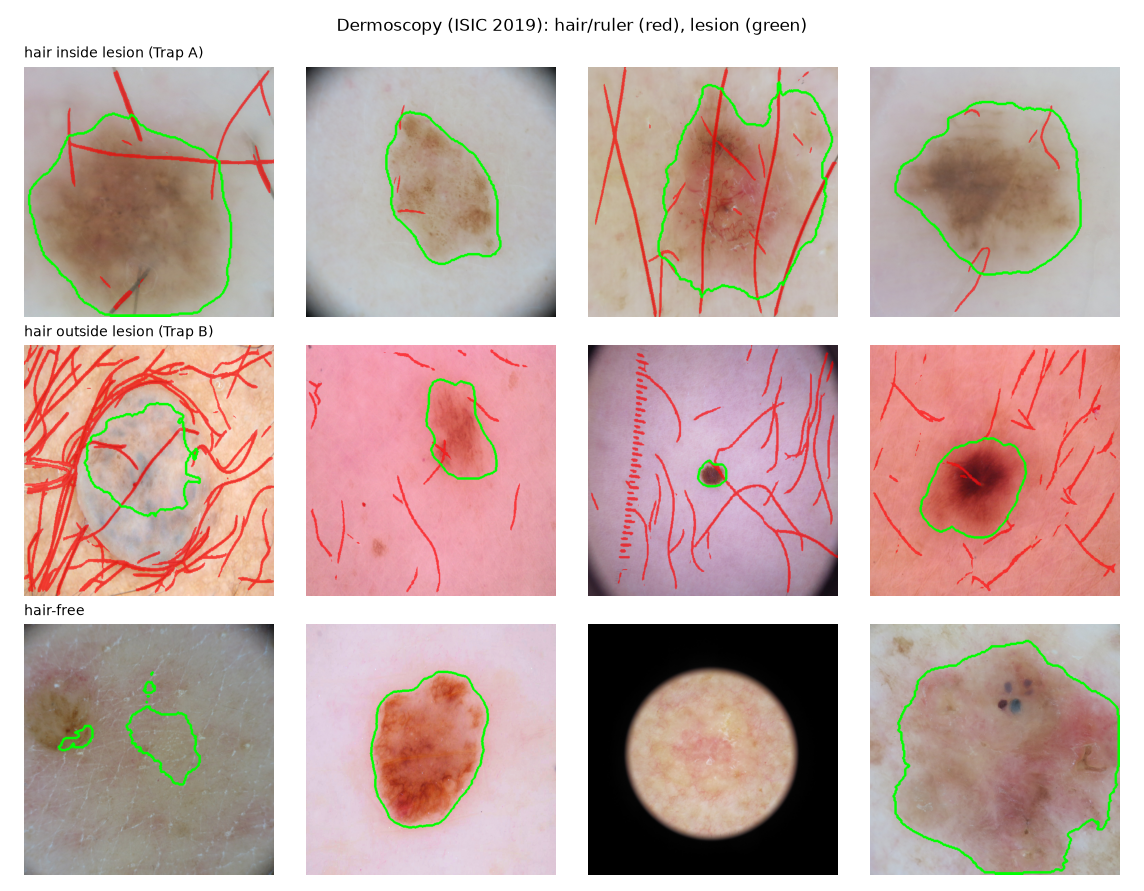
\includegraphics[width=\linewidth]{../figures/data_isic.png}
\caption{ISIC 2019 dermoscopy: real hair inside (Trap A) and outside (Trap B) the lesion.}\label{fig:isic}\end{figure}
\begin{figure}[H]\centering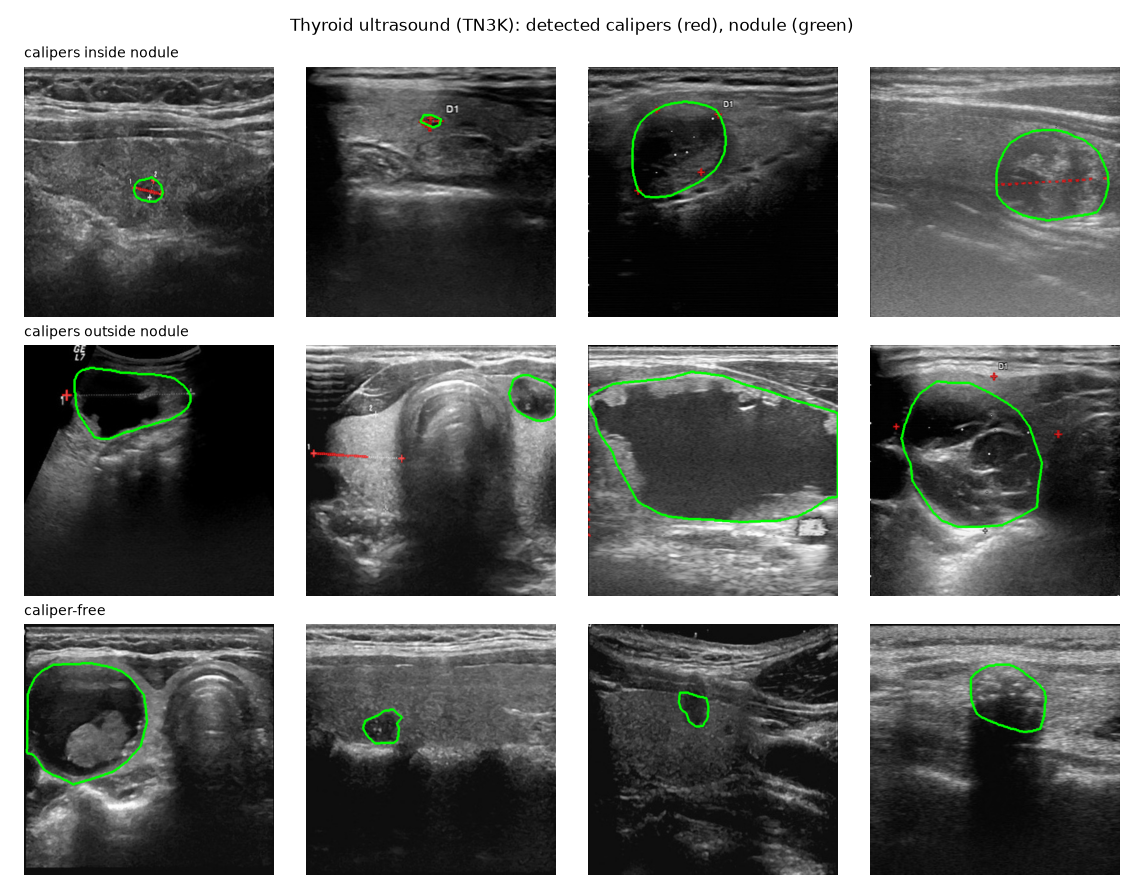
\includegraphics[width=\linewidth]{../figures/data_thyroid.png}
\caption{Thyroid ultrasound (TN3K/TNCD): sonographer calipers on and off the nodule.}\label{fig:thy}\end{figure}
\begin{figure}[H]\centering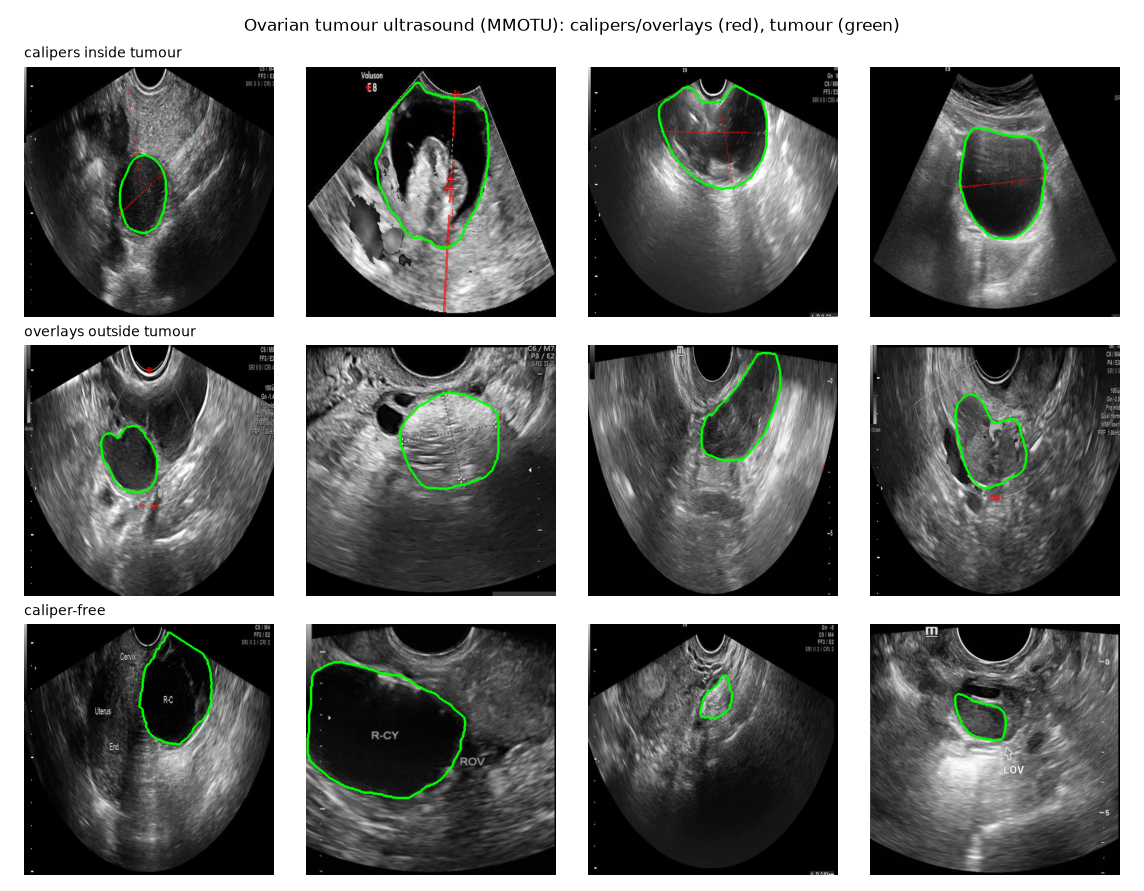
\includegraphics[width=\linewidth]{../figures/data_ovary.png}
\caption{Ovarian ultrasound (MMOTU): calipers and overlays.}\end{figure}
\begin{figure}[H]\centering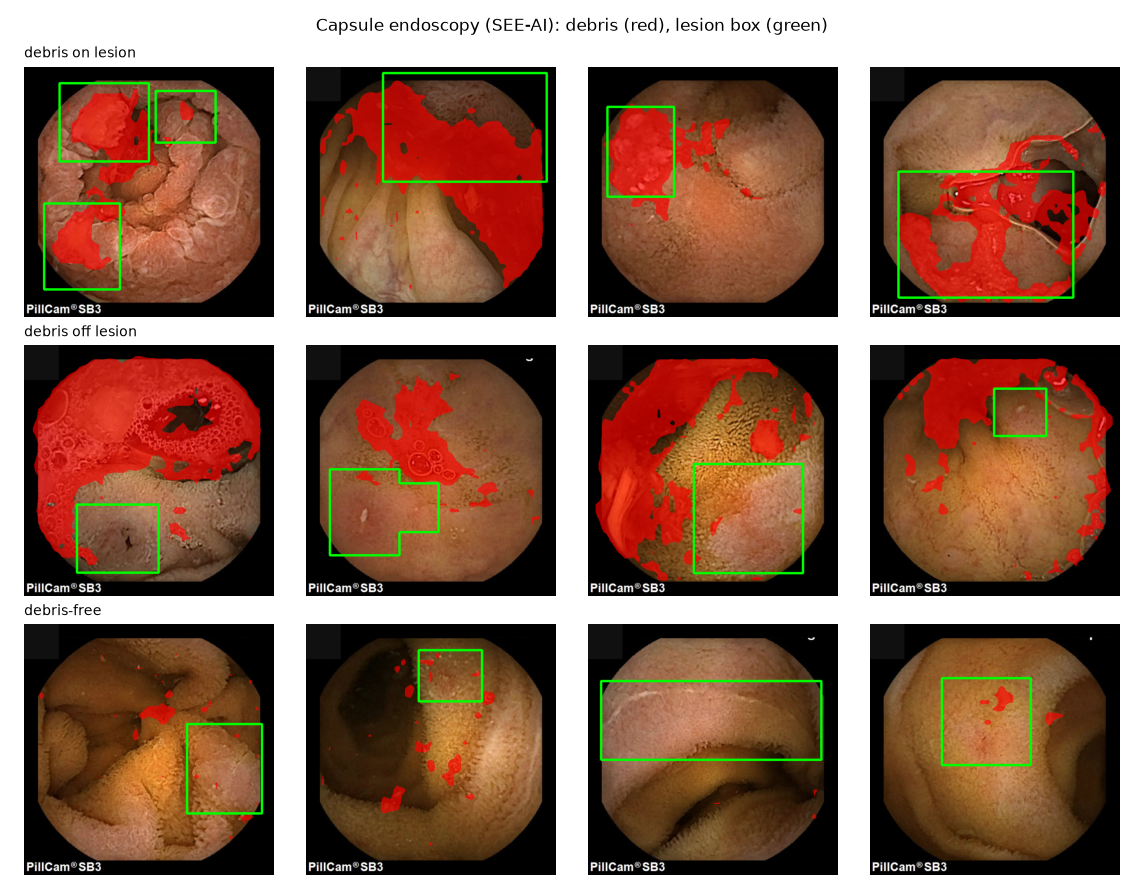
\includegraphics[width=\linewidth]{../figures/data_capsule.png}
\caption{Capsule endoscopy (SEE-AI): debris/bubbles on and off the lesion.}\end{figure}
\begin{figure}[H]\centering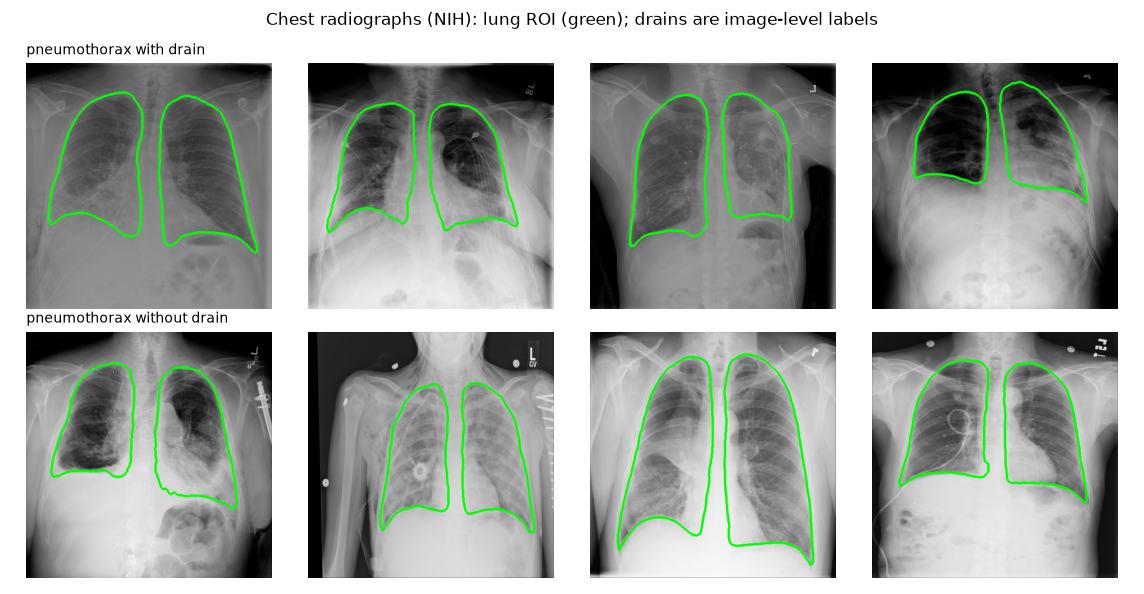
\includegraphics[width=\linewidth]{../figures/data_cxr.png}
\caption{Chest radiography (NIH ChestX-ray14): chest drains and lung masks.}\label{fig:cxr}\end{figure}

\section{Stage 0 --- the pilot and its replication}
\textbf{Question.} Does the original thesis (``Where the Shortcut Sits'') reproduce? \textbf{Design.} The author's
protocol was written down as a specification (registry \S\ref{doc:REPLICATION_SPEC}) and re-implemented from scratch:
E1--E7 controlled rulers on ISIC 2018 (DINOv2 ViT-B/14 @518 and @224, DermLIP), E10 hair decodability, E12 contrast trap,
E13/E15 real hair traps on ISIC 2019, E14 area ratio. \textbf{Result.} 88 numbers compared: 73 MATCH (same sign, same CI
verdict, $|\Delta|\le0.02$), 12 SIGN+CI (same sign and verdict, $|\Delta|>0.02$), 3 MISMATCH (E4 occlusion at 50\% has a CI
that now excludes 0; E12 contrast trap not null; one HAM-only stratum). Full ledger: Appendix~\ref{app:resultsmd}.
\textbf{Thesis-claims audit:} registry \S\ref{doc:THESIS_CLAIMS_AUDIT}. \textbf{Conclusion.} The pilot is reproducible; the
three mismatches are documented and do not affect the central claims.

\section{Stage 1 --- controlled dermoscopy and the mechanism}
\textbf{Design.} 2{,}437 ISIC 2018 images; a synthetic ruler correlated with melanoma (0.9/0.1) pasted at overlap
$r\in\{0,0.25,0.5,0.75,1\}$ with the lesion; DINOv2 ViT-B/14 @518 frozen, logistic heads; seeds 42, 123, 456.
\textbf{Results.} Masking improves reversed AUROC by $+0.184$ [$+0.146,+0.224$] at $r=0$ and lowers it by $-0.097$,
$-0.112$, $-0.129$ at 50/75/100\% (interaction $+0.313$ [$+0.272,+0.353$]); reproduced at 224\,px ($+0.361$ at 0\%,
$-0.095$ at 100\%), with DermLIP (harm $\approx-0.29$ at every in-ROI overlap) and a randomised ruler. At $r=0$ the masked
model's correlated and reversed AUROC coincide (0.849/0.849); at $r=1$ the masked model's correlated AUROC exceeds ERM's
(0.961 vs 0.937) --- it uses the ruler more.
\textbf{Mechanism (three explanations tested separately).} \emph{Occlusion} is not the cause: with the ruler present but
uncorrelated (50/50) masking helps at every overlap ($+0.036$, $+0.040$, $+0.039$). \emph{Lost context} alone is not the
cause: dilating the mask at 50\% overlap increases harm ($-0.097\to-0.138\to-0.154$) as it restores ruler pixels
(retention 0.50$\to$0.73$\to$0.95), and at full overlap harm is flat although the ruler's share of visible pixels falls
threefold. \emph{Retention with amplified reliance}: same-head counterfactual sensitivity to the ruler doubles
(0.235$\to$0.491); harm is largest for small lesions ($-0.364$ vs $+0.064$ for large lesions at 100\%).
Fig.~\ref{fig:mech} shows the same mechanism in all five controlled sweeps.
\begin{figure}[H]\centering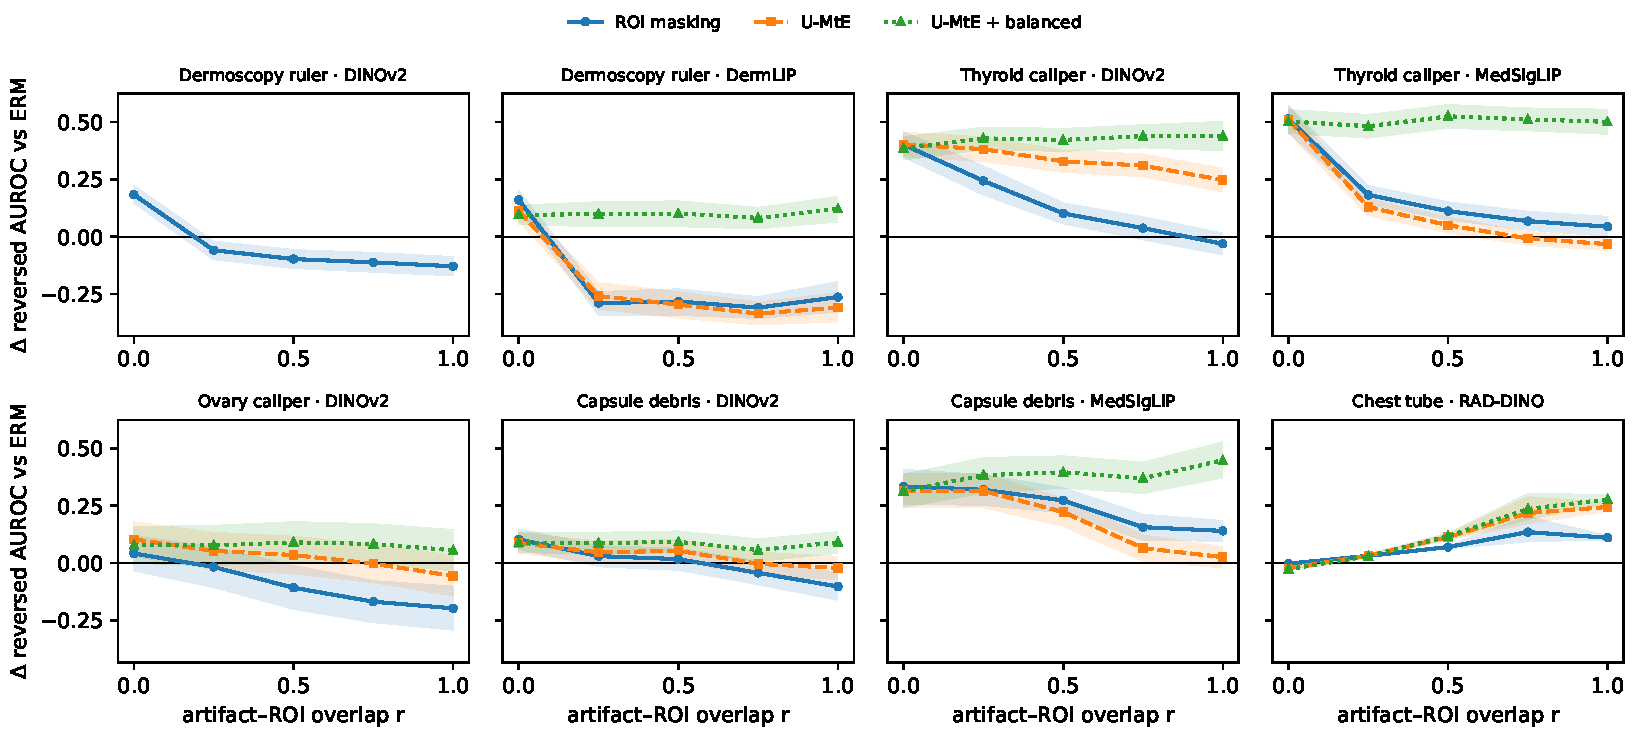
\includegraphics[width=\linewidth]{../../paper/figures/dose_response.pdf}
\caption{Controlled overlap sweeps: $\Delta$ reversed AUROC vs ERM as a synthetic artifact moves into the ROI (95\% CIs).
Masking (blue) declines with overlap except in chest radiography; U-MtE + balancing (green) is flat.}\label{fig:dose}\end{figure}
\begin{figure}[H]\centering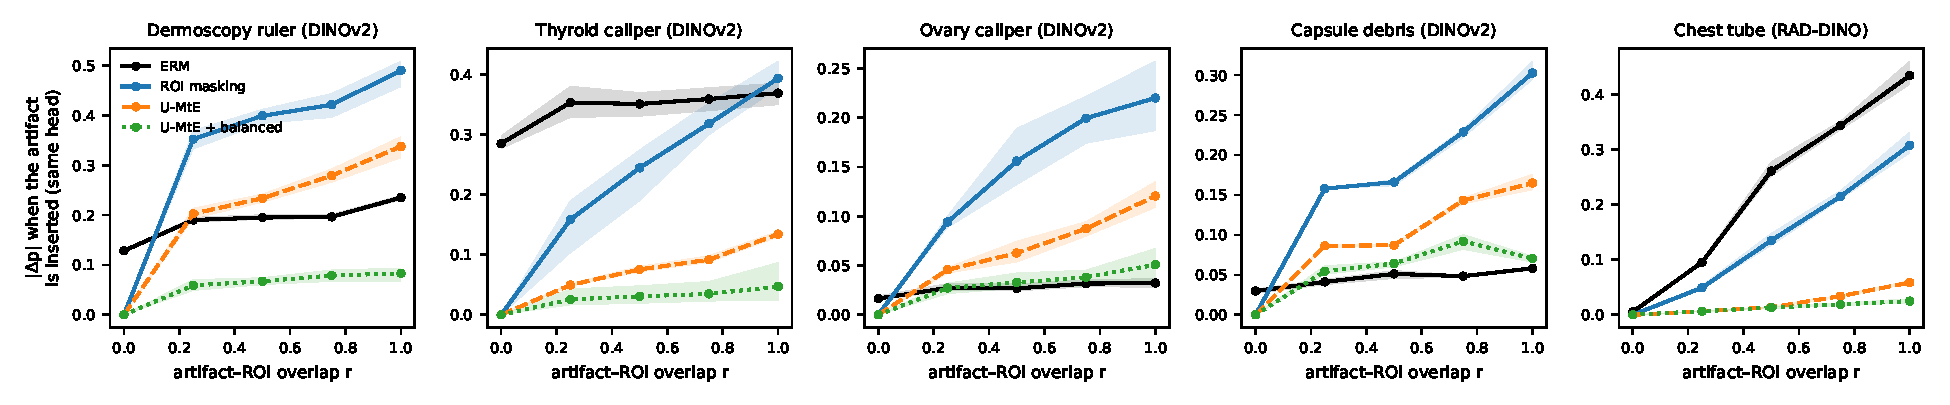
\includegraphics[width=\linewidth]{../../paper/figures/mechanism.pdf}
\caption{Mechanism: counterfactual sensitivity $|p(x{+}\text{artifact})-p(x)|$ vs overlap. Masking increases reliance on an
in-ROI artifact; U-MtE and balancing remove it. At full overlap: dermoscopy 0.491 (mask) vs 0.235 (ERM); ovary 0.218 vs
0.032; capsule 0.302 vs 0.058; thyroid 0.393 vs 0.369; chest tube: ERM ignores extra-pulmonary tubes ($|\Delta p|=0.005$ at
$r=0$).}\label{fig:mech}\end{figure}
\textbf{Leakage assessment (controlled sweep).} Five random splits contained 67--124 near-duplicate pairs across the split;
the grouped split has none. Random splits change the ERM shortcut gap and the size of the masking effect (Table~\ref{tab:leak}),
so every analysis uses grouped splits.
\begin{table}[H]\centering\scriptsize
\caption{Leakage assessment (controlled dermoscopy sweep): grouped (lesion ID + pHash) versus five random splits.}\label{tab:leak}
\begin{tabular}{lccccccc}\toprule
Split & Overlap & Near-dup pairs across split & ERM clean & ERM corr & ERM rev & ERM gap & mask$-$ERM rev \\\midrule
grouped & 0.0 & 0 & 0.797 & 0.906 & 0.665 & 0.241 & 0.184 \\
grouped & 1.0 & 0 & 0.792 & 0.937 & 0.515 & 0.422 & -0.129 \\
random\_0 & 0.0 & 98 & 0.812 & 0.909 & 0.649 & 0.260 & 0.188 \\
random\_0 & 1.0 & 98 & 0.810 & 0.944 & 0.495 & 0.450 & -0.119 \\
random\_1 & 0.0 & 101 & 0.809 & 0.906 & 0.658 & 0.248 & 0.180 \\
random\_1 & 1.0 & 101 & 0.807 & 0.945 & 0.523 & 0.422 & -0.109 \\
random\_2 & 0.0 & 75 & 0.828 & 0.924 & 0.555 & 0.369 & 0.297 \\
random\_2 & 1.0 & 75 & 0.827 & 0.945 & 0.404 & 0.541 & -0.007 \\
random\_3 & 0.0 & 124 & 0.837 & 0.913 & 0.707 & 0.206 & 0.180 \\
random\_3 & 1.0 & 124 & 0.821 & 0.949 & 0.520 & 0.429 & -0.147 \\
random\_4 & 0.0 & 67 & 0.818 & 0.926 & 0.591 & 0.335 & 0.269 \\
random\_4 & 1.0 & 67 & 0.824 & 0.946 & 0.463 & 0.482 & -0.059 \\
\bottomrule\end{tabular}\end{table}


\section{Stage 2 --- real dermoscopic hair (ISIC 2019)}
\textbf{Design} (registry \S\ref{doc:PREREGISTRATION_ISIC2019_TRAPS}). Hair-free group A0 = at most 30 native hair pixels;
Trap A: in-lesion hair ($r\ge0.5$); Trap B: $r<0.1$; cells matched to the A0 source mix; five seeds (42, 123, 456, 789,
2026) $\times$ five group-safe folds (lesion ID + pHash); 172 reversed-test melanomas per trap and seed.
\textbf{Results.} Masking helps in Trap B ($+0.107$ [$+0.078,+0.135$]) and harms in Trap A ($-0.037$ [$-0.057,-0.019$],
negative in all five seeds); crossover $+0.145$ [$+0.105,+0.181$]. Harm holds in BCN ($-0.051$) but not HAM ($-0.009$, n.s.).
Oracle hair inpainting helps both traps ($+0.103$/$+0.096$). Group-balanced training and DFR (image-level hair label) give
the largest gains ($+0.225$/$+0.251$ Trap A; $+0.209$/$+0.215$ Trap B); paired LEACE recovers less than half.
Hair is decodable from the embedding (AUROC 0.943) but removing every hair patch with the oracle mask gains only
$+0.015$: the hair shortcut is mostly carried by correlates (body site, age, sex; registry \S\ref{doc:PREREGISTRATION_ISIC2019_TRAPS}).
\textbf{Conclusion.} In-ROI masking harms on real data; hair is the \emph{correlate-carried} regime.

\section{Stage 3 --- chest radiography, the boundary case}
\textbf{Controlled tube sweep} (NIH pneumothorax, RAD-DINO): no sign reversal --- ERM does not use a tube outside the
lungs ($|\Delta p|=0.005$ at $r=0$), so masking has nothing to remove there; inside the lungs masking reduces but does not
remove reliance. \textbf{Real chest drains} (29{,}687 images, patient-grouped folds; registry \S\ref{doc:PREREGISTRATION_CXR_DRAIN}):
an extreme shortcut (ERM reversed 0.19 RAD-DINO, 0.28 DINOv2); lung masking $+0.05$/$+0.01$; U-MtE $+0.03$ over masking
(RAD-DINO only); DFR and mask+DFR best --- a drain comes with a treated lung (correlate-carried). \textbf{Pathology traps with
real devices} (Atelectasis, Consolidation, Effusion, Infiltration; registry \S\ref{doc:PREREGISTRATION_CXR_DEVICE_TRAPS}):
crossovers near zero ($+0.060$, $-0.002$, $-0.004$, $-0.032$). \textbf{Conclusion.} Chest radiography is reported as a boundary
case, not as a fifth confirmation.

\section{Stage 4 --- new modalities: thyroid, ovarian and capsule traps}
\textbf{Artifact labels without annotation.} Calipers: a rule-based detector (colour/shape; visual audit: 95\% of thyroid
detections on real calipers, 92--97\% of caliper-free images clean; registry \S\ref{doc:THYROID_MARKER_AUDIT},
\S\ref{doc:ARTIFACT_MASK_AUDIT}). Capsule debris: a patch-token probe trained on the published expert contamination masks
(IoU 0.62). \textbf{Traps} as in Stage 2 (five seeds $\times$ five folds). \textbf{Results (DINOv2).}
\begin{table}[H]\centering\small\caption{Masking gain (reversed AUROC) by artifact location, DINOv2 ViT-B/14 @518.}
\begin{tabular}{lccc}\toprule Cohort & mask$-$ERM, Trap A (in-ROI) & mask$-$ERM, Trap B (out) & Crossover \\\midrule
ISIC hair & $-0.037$ [$-0.057,-0.019$] & $+0.107$ [$+0.078,+0.135$] & $+0.145$ [$+0.105,+0.181$] \\
Thyroid calipers & $+0.111$ [$+0.097,+0.124$] & $+0.341$ [$+0.320,+0.363$] & $+0.230$ [$+0.204,+0.255$] \\
Ovarian calipers & $+0.132$ [$+0.089,+0.174$] & $+0.302$ [$+0.261,+0.343$] & $+0.170$ [$+0.116,+0.224$] \\
Capsule debris & $+0.096$ [$+0.081,+0.113$] & $+0.465$ [$+0.440,+0.490$] & $+0.368$ [$+0.340,+0.397$] \\\bottomrule
\end{tabular}\end{table}
\textbf{Controlled sweeps in the same cohorts} (synthetic caliper/debris pasted at controlled overlap): ovary at full
overlap $-0.197$ [$-0.292,-0.100$], capsule $-0.102$ [$-0.162,-0.040$], thyroid $-0.030$ (n.s.); location interactions
capsule $+0.205$, thyroid $+0.432$. \textbf{Observation.} On real thyroid/ovary/capsule, in-ROI masking still helps a
little (it removes clutter) --- the universal claim is the \emph{gap} (crossover), and harm appears whenever masking also
removes disease context (dermoscopy, sweeps, fine-tuned capsule, unaltered data).

\section{Stage 5 --- the confirmatory primary family}
Each test was pre-registered individually; the family of 16 (four hypotheses $\times$ four cohorts, DINOv2) was defined
afterwards for multiplicity control and corrected with Holm (BH for reference; registry \S\ref{doc:STATISTICAL_PLAN}).
\begin{table}[H]\centering\small
\caption{The 16 pre-registered primary tests (DINOv2 ViT-B/14 @518; reversed-test AUROC; Holm over the family).}\label{tab:primary}
\begin{tabular}{llccc}\toprule
Family & Cohort & Estimate [95\% CI] & $p_{\text{Holm}}$ & Supported \\\midrule
P1 location crossover & ISIC hair (DINOv2) & +0.145 [+0.105, +0.181] & 0.0016 & yes \\
P1 location crossover & Thyroid (DINOv2) & +0.230 [+0.204, +0.255] & 0.0016 & yes \\
P1 location crossover & Capsule (DINOv2) & +0.368 [+0.340, +0.397] & 0.0016 & yes \\
P1 location crossover & Ovary (DINOv2) & +0.170 [+0.116, +0.224] & 0.0016 & yes \\
P2 U-MtE (protected) > mask & ISIC hair & +0.041 [+0.030, +0.054] & 0.0016 & yes \\
P2 U-MtE (protected) > mask & Thyroid & +0.217 [+0.174, +0.257] & 0.0016 & yes \\
P2 U-MtE (protected) > mask & Capsule & -0.010 [-0.021, -0.001] & 0.0900 & no \\
P2 U-MtE (protected) > mask & Ovary & +0.043 [+0.026, +0.061] & 0.0016 & yes \\
P3 erase > augment & ISIC hair & +0.045 [+0.037, +0.054] & 0.0016 & yes \\
P3 erase > augment & Thyroid & +0.207 [+0.182, +0.235] & 0.0016 & yes \\
P3 erase > augment & Capsule & -0.130 [-0.147, -0.110] & 0.0016 & no \\
P3 erase > augment & Ovary & +0.035 [+0.010, +0.059] & 0.0224 & yes \\
P4 U-MtE+balanced > balanced & ISIC hair & -0.013 [-0.041, +0.018] & 0.4230 & no \\
P4 U-MtE+balanced > balanced & Thyroid & +0.112 [+0.090, +0.134] & 0.0016 & yes \\
P4 U-MtE+balanced > balanced & Capsule & +0.082 [+0.064, +0.100] & 0.0016 & yes \\
P4 U-MtE+balanced > balanced & Ovary & +0.028 [+0.000, +0.057] & 0.0988 & no \\
\bottomrule\end{tabular}\end{table}

\begin{figure}[H]\centering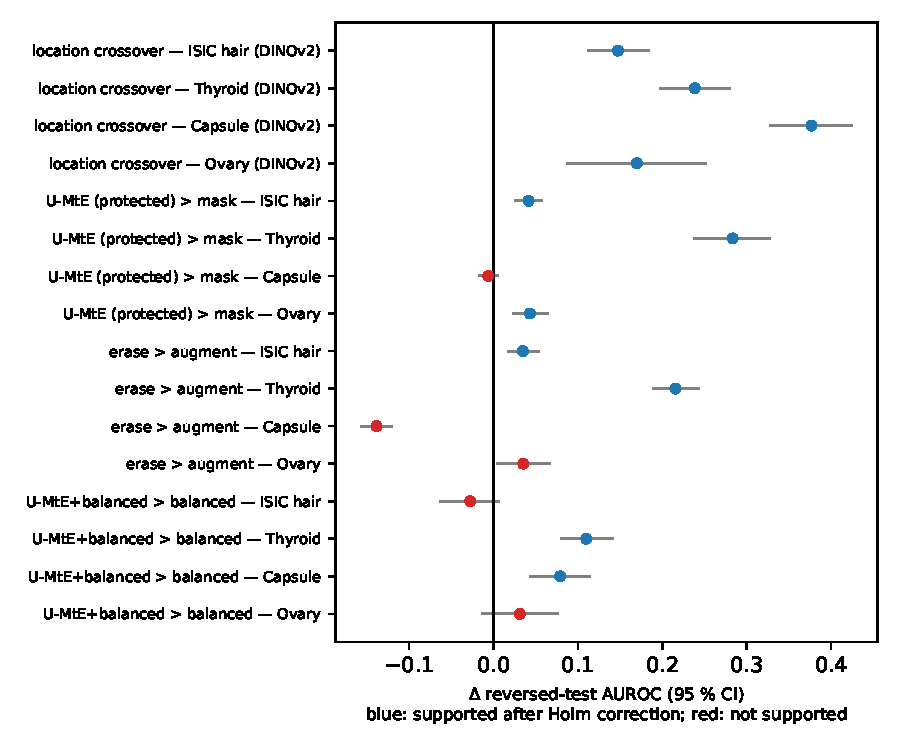
\includegraphics[width=0.8\linewidth]{../../paper/figures/forest.pdf}
\caption{Forest plot of the 16 primary tests (blue: supported after Holm).}\end{figure}

\section{Stage 6 --- replication breadth: backbones, scale, foundation models}
\textbf{Backbone families.} Thyroid crossover $+0.163$ (MedSigLIP), $+0.284$ (ConvNeXt); capsule $+0.332$ (MedSigLIP),
$+0.292$ (ConvNeXt); ovary $+0.179$ (MedSigLIP). \textbf{Scale} (DINOv2 ViT-S/B/L; registry \S\ref{doc:PREREGISTRATION_SCALE}):
\begin{table}[H]\centering\scriptsize
\caption{Backbone scale (Trap A for the U-MtE contrasts; ERM gap = correlated $-$ reversed AUROC, Trap A).}\label{tab:scale}
\begin{tabular}{llcccc}\toprule
Cohort & DINOv2 & Crossover & U-MtE$_{\text{prot}}-$mask & U-MtE$-$mask & ERM gap \\\midrule
thyroid & ViT-S/14 & +0.244 [+0.209, +0.275] & +0.181 [+0.146, +0.218] & +0.182 [+0.144, +0.213] & 0.547 \\
thyroid & ViT-B/14 & +0.230 [+0.204, +0.255] & +0.217 [+0.174, +0.257] & +0.222 [+0.196, +0.251] & 0.590 \\
thyroid & ViT-L/14 & +0.271 [+0.234, +0.308] & +0.222 [+0.195, +0.256] & +0.213 [+0.188, +0.235] & 0.621 \\
ovary & ViT-S/14 & +0.298 [+0.229, +0.365] & +0.103 [+0.078, +0.128] & +0.120 [+0.092, +0.147] & 0.319 \\
ovary & ViT-B/14 & +0.170 [+0.116, +0.224] & +0.043 [+0.026, +0.061] & +0.019 [-0.007, +0.044] & 0.409 \\
ovary & ViT-L/14 & +0.202 [+0.153, +0.250] & +0.060 [+0.043, +0.077] & +0.094 [+0.071, +0.118] & 0.570 \\
capsule & ViT-S/14 & +0.370 [+0.341, +0.401] & -0.008 [-0.014, -0.003] & -0.153 [-0.167, -0.140] & 0.353 \\
capsule & ViT-B/14 & +0.368 [+0.340, +0.397] & -0.010 [-0.021, -0.001] & -0.115 [-0.128, -0.101] & 0.354 \\
capsule & ViT-L/14 & +0.408 [+0.378, +0.438] & -0.040 [-0.046, -0.035] & -0.093 [-0.103, -0.083] & 0.325 \\
\bottomrule\end{tabular}\end{table}

Larger models exploit the in-ROI caliper shortcut \emph{more} (ERM gap thyroid 0.547$\to$0.621, ovary 0.319$\to$0.570).
\textbf{Zero-shot vision--language models} (no training; registry \S\ref{doc:PREREGISTRATION_TEXT_PROMPT}): zero-shot
scores are already swayed by artifacts (capsule correlated$-$reversed gap 0.40) and masking changes them per the location
law: crossovers thyroid $+0.103$ [$+0.079,+0.127$], capsule $+0.049$ [$+0.024,+0.076$], ovary $+0.181$ [$+0.135,+0.228$]
(MedSigLIP), hair $+0.051$ [$+0.031,+0.071$] (DermLIP). Caveat: MedSigLIP zero-shot thyroid classification is at chance
(clean 0.45). \textbf{Conclusion.} The effect is a property of the representation, not of the trained head.

\section{Stage 7 --- unaltered test distributions and clinical metrics}
\textbf{Design} (registry \S\ref{doc:PREREGISTRATION_NATURAL}). No resampling. Thyroid: official TN3K split; ISIC 2019:
each hospital (BCN, HAM, MSK) held out in turn; capsule: held-out frame-block groups (per seed). Natural associations:
thyroid calipers 37.6\% of benign vs 24.1\% of malignant; in-lesion hair 31\% of melanomas vs 20\% of benign; capsule debris
on lesion 23\% of polyp-like vs 10\% of erosions. ``Hard'' pairs = shortcut-conflicting pairs.
\begin{table}[H]\centering\scriptsize
\caption{Natural (unaltered) test distributions: every bootstrap contrast (hard = shortcut-conflicting pairs).}\label{tab:natural}
\begin{tabular}{lll}\toprule
Test set & Subset $|$ contrast & $\Delta$ AUROC [95\% CI] \\\midrule
capsule & hard $|$ mask-erm & +0.021 [+0.000, +0.044] \\
capsule & hard $|$ mte-mask & +0.000 [-0.010, +0.009] \\
capsule & hard $|$ mte\_protect-mask & -0.024 [-0.035, -0.014] \\
capsule & hard $|$ balanced-mask & -0.009 [-0.031, +0.011] \\
capsule & hard $|$ mte\_balanced-mask & +0.014 [+0.003, +0.025] \\
capsule & easy $|$ mask-erm & +0.071 [+0.042, +0.104] \\
capsule & easy $|$ mte-mask & -0.001 [-0.009, +0.007] \\
capsule & easy $|$ mte\_protect-mask & -0.021 [-0.030, -0.014] \\
capsule & easy $|$ balanced-mask & -0.079 [-0.123, -0.046] \\
capsule & easy $|$ mte\_balanced-mask & -0.008 [-0.016, +0.000] \\
capsule & all $|$ mask-erm & +0.077 [+0.062, +0.093] \\
capsule & all $|$ mte-mask & -0.005 [-0.010, +0.000] \\
capsule & all $|$ mte\_protect-mask & -0.022 [-0.026, -0.018] \\
capsule & all $|$ balanced-mask & -0.086 [-0.106, -0.067] \\
capsule & all $|$ mte\_balanced-mask & -0.008 [-0.013, -0.002] \\
isic BCN & hard $|$ mask-erm & -0.016 [-0.027, -0.005] \\
isic BCN & hard $|$ mte-mask & +0.003 [+0.000, +0.006] \\
isic BCN & hard $|$ mte\_protect-mask & -0.002 [-0.007, +0.002] \\
isic BCN & hard $|$ balanced-mask & +0.034 [+0.023, +0.045] \\
isic BCN & hard $|$ mte\_balanced-mask & +0.034 [+0.029, +0.039] \\
isic BCN & easy $|$ mask-erm & -0.012 [-0.021, -0.004] \\
isic BCN & easy $|$ mte-mask & +0.003 [-0.000, +0.006] \\
isic BCN & easy $|$ mte\_protect-mask & -0.024 [-0.029, -0.019] \\
isic BCN & easy $|$ balanced-mask & -0.008 [-0.017, +0.001] \\
isic BCN & easy $|$ mte\_balanced-mask & -0.018 [-0.023, -0.014] \\
isic BCN & all $|$ mask-erm & -0.016 [-0.021, -0.012] \\
isic BCN & all $|$ mte-mask & +0.004 [+0.002, +0.006] \\
isic BCN & all $|$ mte\_protect-mask & -0.014 [-0.017, -0.011] \\
isic BCN & all $|$ balanced-mask & +0.011 [+0.006, +0.016] \\
isic BCN & all $|$ mte\_balanced-mask & +0.004 [+0.002, +0.006] \\
isic HAM & hard $|$ mask-erm & +0.053 [+0.037, +0.068] \\
isic HAM & hard $|$ mte-mask & +0.023 [+0.017, +0.032] \\
isic HAM & hard $|$ mte\_protect-mask & -0.043 [-0.055, -0.031] \\
isic HAM & hard $|$ balanced-mask & -0.022 [-0.038, -0.006] \\
isic HAM & hard $|$ mte\_balanced-mask & +0.065 [+0.056, +0.075] \\
isic HAM & easy $|$ mask-erm & +0.015 [+0.002, +0.028] \\
isic HAM & easy $|$ mte-mask & -0.001 [-0.015, +0.010] \\
isic HAM & easy $|$ mte\_protect-mask & +0.013 [+0.004, +0.024] \\
isic HAM & easy $|$ balanced-mask & -0.041 [-0.061, -0.021] \\
isic HAM & easy $|$ mte\_balanced-mask & -0.024 [-0.030, -0.017] \\
isic HAM & all $|$ mask-erm & +0.040 [+0.033, +0.046] \\
isic HAM & all $|$ mte-mask & +0.010 [+0.004, +0.014] \\
isic HAM & all $|$ mte\_protect-mask & -0.011 [-0.018, -0.005] \\
isic HAM & all $|$ balanced-mask & -0.042 [-0.054, -0.026] \\
isic HAM & all $|$ mte\_balanced-mask & +0.013 [+0.008, +0.017] \\
isic MSK & hard $|$ mask-erm & -0.056 [-0.084, -0.029] \\
isic MSK & hard $|$ mte-mask & -0.008 [-0.015, -0.002] \\
isic MSK & hard $|$ mte\_protect-mask & +0.032 [+0.023, +0.042] \\
isic MSK & hard $|$ balanced-mask & +0.094 [+0.069, +0.119] \\
isic MSK & hard $|$ mte\_balanced-mask & +0.041 [+0.029, +0.053] \\
isic MSK & easy $|$ mask-erm & +0.099 [+0.080, +0.118] \\
isic MSK & easy $|$ mte-mask & +0.001 [-0.005, +0.007] \\
isic MSK & easy $|$ mte\_protect-mask & -0.027 [-0.034, -0.020] \\
isic MSK & easy $|$ balanced-mask & -0.132 [-0.153, -0.111] \\
isic MSK & easy $|$ mte\_balanced-mask & -0.028 [-0.036, -0.021] \\
isic MSK & all $|$ mask-erm & +0.021 [+0.010, +0.031] \\
isic MSK & all $|$ mte-mask & -0.007 [-0.010, -0.004] \\
isic MSK & all $|$ mte\_protect-mask & -0.004 [-0.008, +0.001] \\
isic MSK & all $|$ balanced-mask & -0.024 [-0.035, -0.013] \\
isic MSK & all $|$ mte\_balanced-mask & -0.016 [-0.021, -0.011] \\
thyroid & hard $|$ mask-erm & -0.102 [-0.139, -0.066] \\
thyroid & hard $|$ mte-mask & +0.051 [+0.033, +0.072] \\
thyroid & hard $|$ mte\_protect-mask & -0.058 [-0.079, -0.036] \\
thyroid & hard $|$ balanced-mask & +0.142 [+0.107, +0.178] \\
thyroid & hard $|$ mte\_balanced-mask & +0.088 [+0.071, +0.108] \\
thyroid & easy $|$ mask-erm & +0.048 [+0.019, +0.079] \\
thyroid & easy $|$ mte-mask & -0.010 [-0.028, +0.004] \\
thyroid & easy $|$ mte\_protect-mask & +0.010 [-0.005, +0.023] \\
thyroid & easy $|$ balanced-mask & -0.115 [-0.146, -0.084] \\
thyroid & easy $|$ mte\_balanced-mask & -0.049 [-0.066, -0.035] \\
thyroid & all $|$ mask-erm & -0.005 [-0.027, +0.018] \\
thyroid & all $|$ mte-mask & +0.010 [+0.002, +0.018] \\
thyroid & all $|$ mte\_protect-mask & -0.017 [-0.027, -0.007] \\
thyroid & all $|$ balanced-mask & -0.015 [-0.039, +0.008] \\
thyroid & all $|$ mte\_balanced-mask & -0.000 [-0.009, +0.008] \\
\bottomrule\end{tabular}\end{table}

\begin{table}[t]\centering\scriptsize
\caption{Clinical secondary metrics on the unaltered test sets (Table~\ref{m:tab:natural}): mean (SD) over training seeds. Sensitivity and specificity at the operating point fixed on clean validation data; ECE with 10 equal-width bins; AUPRC baseline = prevalence.}\label{tab:natural_clinical}
\begin{tabular}{llcccccc}\toprule
Test set & Arm & AUROC & AUPRC & Brier & ECE & Sens & Spec \\\midrule
Thyroid (official split) ($\pi=0.38$) & ERM & 0.736 (0.009) & 0.606 (0.012) & 0.207 (0.005) & 0.082 (0.008) & 0.734 (0.047) & 0.619 (0.061) \\
 & mask & 0.731 (0.006) & 0.632 (0.007) & 0.214 (0.006) & 0.120 (0.026) & 0.347 (0.095) & 0.888 (0.041) \\
 & U-MtE & 0.742 (0.003) & 0.638 (0.007) & 0.203 (0.001) & 0.085 (0.007) & 0.425 (0.088) & 0.854 (0.050) \\
 & balanced & 0.716 (0.007) & 0.584 (0.012) & 0.219 (0.004) & 0.110 (0.007) & 0.714 (0.052) & 0.599 (0.061) \\
 & U-MtE$_{\text{bal}}$ & 0.731 (0.004) & 0.630 (0.007) & 0.207 (0.001) & 0.084 (0.006) & 0.399 (0.069) & 0.866 (0.034) \\
\midrule
ISIC, BCN held out ($\pi=0.23$) & ERM & 0.786 (0.003) & 0.586 (0.003) & 0.239 (0.006) & 0.279 (0.011) & 0.842 (0.038) & 0.519 (0.075) \\
 & mask & 0.769 (0.004) & 0.571 (0.009) & 0.286 (0.007) & 0.332 (0.009) & 0.860 (0.013) & 0.439 (0.023) \\
 & U-MtE & 0.773 (0.004) & 0.574 (0.008) & 0.280 (0.009) & 0.328 (0.012) & 0.858 (0.039) & 0.448 (0.089) \\
 & balanced & 0.781 (0.005) & 0.585 (0.009) & 0.228 (0.006) & 0.257 (0.011) & 0.811 (0.046) & 0.554 (0.087) \\
 & U-MtE$_{\text{bal}}$ & 0.774 (0.004) & 0.568 (0.008) & 0.279 (0.011) & 0.325 (0.016) & 0.860 (0.027) & 0.447 (0.051) \\
\midrule
ISIC, MSK held out ($\pi=0.19$) & ERM & 0.770 (0.008) & 0.477 (0.012) & 0.172 (0.007) & 0.161 (0.019) & 0.608 (0.049) & 0.786 (0.039) \\
 & mask & 0.790 (0.004) & 0.512 (0.009) & 0.146 (0.003) & 0.115 (0.009) & 0.593 (0.052) & 0.824 (0.037) \\
 & U-MtE & 0.783 (0.004) & 0.500 (0.008) & 0.150 (0.003) & 0.126 (0.009) & 0.566 (0.073) & 0.831 (0.049) \\
 & balanced & 0.766 (0.008) & 0.462 (0.014) & 0.178 (0.008) & 0.170 (0.020) & 0.626 (0.047) & 0.755 (0.046) \\
 & U-MtE$_{\text{bal}}$ & 0.774 (0.006) & 0.482 (0.009) & 0.154 (0.004) & 0.131 (0.010) & 0.594 (0.061) & 0.798 (0.051) \\
\midrule
ISIC, HAM held out ($\pi=0.11$) & ERM & 0.750 (0.005) & 0.353 (0.005) & 0.162 (0.006) & 0.234 (0.011) & 0.535 (0.092) & 0.813 (0.068) \\
 & mask & 0.789 (0.002) & 0.404 (0.006) & 0.143 (0.005) & 0.217 (0.011) & 0.559 (0.112) & 0.842 (0.063) \\
 & U-MtE & 0.799 (0.008) & 0.406 (0.009) & 0.145 (0.007) & 0.226 (0.016) & 0.573 (0.067) & 0.846 (0.041) \\
 & balanced & 0.747 (0.017) & 0.346 (0.019) & 0.156 (0.014) & 0.228 (0.015) & 0.539 (0.078) & 0.803 (0.076) \\
 & U-MtE$_{\text{bal}}$ & 0.802 (0.005) & 0.401 (0.009) & 0.139 (0.006) & 0.215 (0.021) & 0.606 (0.054) & 0.825 (0.037) \\
\midrule
Capsule (held-out frames) ($\pi=0.56$) & ERM & 0.889 (0.019) & 0.897 (0.046) & 0.130 (0.016) & 0.042 (0.011) & 0.770 (0.062) & 0.844 (0.055) \\
 & mask & 0.967 (0.011) & 0.971 (0.014) & 0.069 (0.013) & 0.029 (0.011) & 0.859 (0.032) & 0.933 (0.025) \\
 & U-MtE & 0.962 (0.009) & 0.967 (0.013) & 0.081 (0.017) & 0.065 (0.045) & 0.871 (0.042) & 0.897 (0.043) \\
 & balanced & 0.881 (0.024) & 0.889 (0.053) & 0.136 (0.017) & 0.051 (0.009) & 0.758 (0.087) & 0.838 (0.059) \\
 & U-MtE$_{\text{bal}}$ & 0.959 (0.008) & 0.964 (0.012) & 0.079 (0.007) & 0.044 (0.012) & 0.866 (0.048) & 0.897 (0.052) \\
\bottomrule
\end{tabular}\end{table}

\textbf{Observations.} Masking lowers AUROC on shortcut-conflicting pairs for thyroid ($-0.102$) and two of three held-out
hospitals; U-MtE$_{\text{bal}}$ improves on masking in every cohort ($+0.014$ to $+0.088$). Pre-registered N1/N2 (protected
U-MtE on thyroid) were \emph{not} supported. Integrity note: the thyroid prediction archive failed a gzip CRC check and was
regenerated deterministically; every number was identical.

\section{Stage 8 --- theory}
\textbf{Closed form} (registry \S\ref{doc:THEORY}): disease block SNR $S$, artifact SNR $A$, training rates $(p_1,p_0)$;
effective artifact SNR $\tilde A=(p_1-p_0)^2A/(1+p_1(1-p_1)A)$ and $\mathrm{AUROC}_{\text{rev}}=\Phi\big((S-\tilde A)/\sqrt{2(S+\tilde A)}\big)$.
Consequences: out-of-ROI masking sets $\tilde A\to0$; in-ROI masking keeps $\tilde A$ and harms iff it removes disease signal
($S_m<S$); the crossover is positive for every $S_m$; erasure scales $S$ by $1-\rho^2$ (fails for pathology-like artifacts
unless protected); group balancing is location-invariant; correlate-carried shortcuts survive masking and erasure.
Simulation agreement $\le0.009$ AUROC over 29 settings (Fig.~\ref{fig:theory}).
\textbf{Real-encoder test} (pre-registered; registry \S\ref{doc:PREREGISTRATION_THEORY_PREDICTION}): the general form for
any test composition was fitted per model to clean and correlated AUROC only, and compared with held-out reversed AUROC.
\begin{table}[H]\centering\small\caption{Theory-vs-real summary (prediction\_summary.json).}\label{tab:theorys}\begin{tabular}{lccc}\toprule Endpoint & Theory & Ref.\ rev$=$clean & Ref.\ rev$=2\cdot$clean$-$corr\\
\midrule
T1 reversed AUROC, ERM+mask (148 models): MAE & 0.039 & 0.234 & 0.108\\
T1 Pearson $r$ & 0.917 & 0.592 & 0.763\\
T1 all ERM-head arms (570): MAE & 0.031 & 0.163 & 0.069\\
T2 crossover (14 pairs): $r$ / MAE / signs & 0.997 / 0.014 / 13 & 0.930 / 0.108 / 12 & 0.989 / 0.036 / 13\\
T3 sweeps (45 points): $r$ / MAE / signs & 0.965 / 0.043 / 42 & 0.670 / 0.122 / 31 & 0.869 / 0.081 / 36\\
T4 in-ROI sign from $S_m-S$ & 11/14 & & \\
Fine-tuned (outside model): rev MAE & 0.018 & & \\
\bottomrule\end{tabular}\par\smallskip Pre-registered verdict: \textbf{qualitative account}.\end{table}

\begin{table}[H]\centering\small
\caption{Theory versus real encoders: location crossover implied by $(S,A)$ fitted to clean and correlated AUROC only.}\label{tab:theoryx}
\begin{tabular}{lllcc}\toprule
Cohort & Backbone & Regime & Observed crossover & Theory (fit on clean+corr) \\\midrule
CXR Atelectasis & RAD-DINO & frozen & +0.060 & +0.062 \\
CXR Consolidation & RAD-DINO & frozen & -0.002 & +0.010 \\
CXR Effusion & RAD-DINO & frozen & -0.004 & -0.013 \\
CXR Infiltration & RAD-DINO & frozen & -0.032 & -0.040 \\
Capsule & ConvNeXt & frozen & +0.292 & +0.288 \\
Capsule & DINOv2 & frozen & +0.368 & +0.335 \\
Capsule & MedSigLIP & frozen & +0.332 & +0.300 \\
Capsule & ResNet-50 FT & end-to-end & +0.584 & +0.542 \\
ISIC hair & DINOv2 & frozen & +0.145 & +0.147 \\
ISIC hair & DermLIP & frozen & -0.002 & -0.003 \\
Ovary & DINOv2 & frozen & +0.170 & +0.157 \\
Ovary & MedSigLIP & frozen & +0.179 & +0.177 \\
Ovary & ResNet-50 FT & end-to-end & +0.136 & +0.096 \\
Thyroid & ConvNeXt & frozen & +0.284 & +0.250 \\
Thyroid & DINOv2 & frozen & +0.230 & +0.204 \\
Thyroid & MedSigLIP & frozen & +0.163 & +0.146 \\
Thyroid & ResNet-50 FT & end-to-end & +0.057 & +0.054 \\
Thyroid & ViT-S FT & end-to-end & +0.168 & +0.114 \\
\bottomrule\end{tabular}\end{table}

\begin{figure}[H]\centering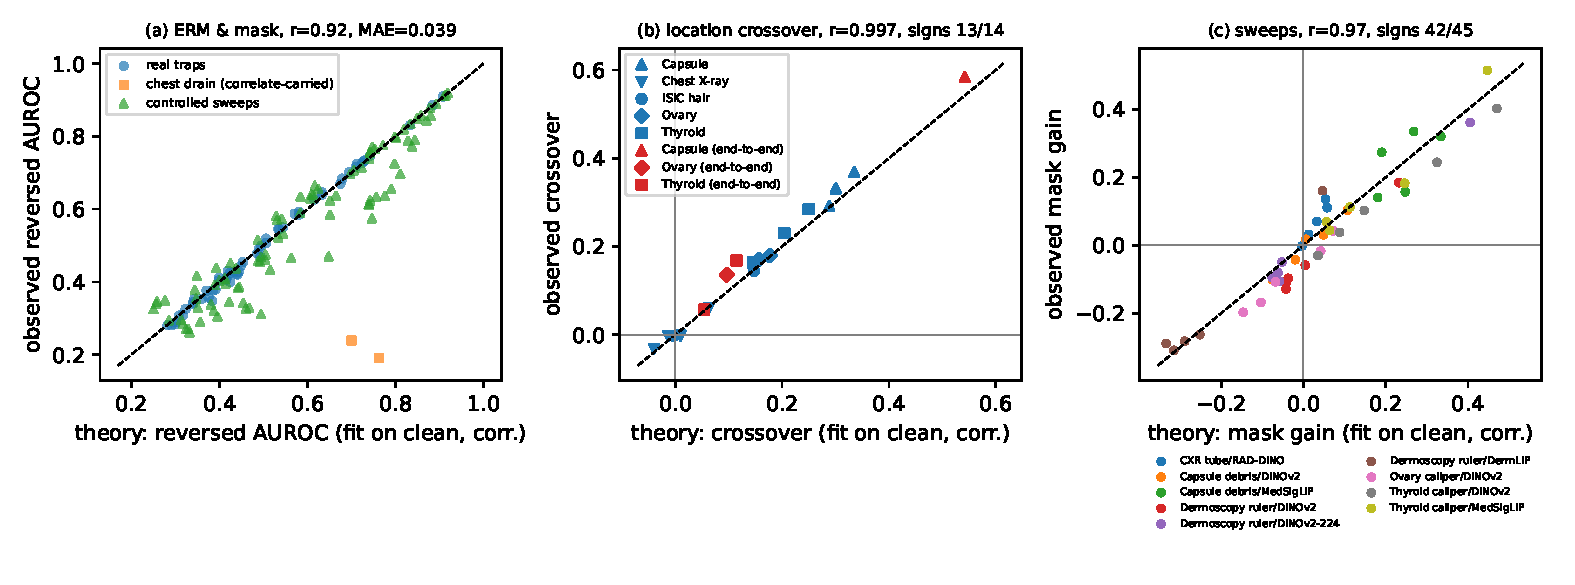
\includegraphics[width=\linewidth]{../../paper/figures/theory_predict.pdf}
\caption{Theory vs real encoders: (a) reversed AUROC; (b) location crossover; (c) sweep mask gains.}\end{figure}
\begin{figure}[H]\centering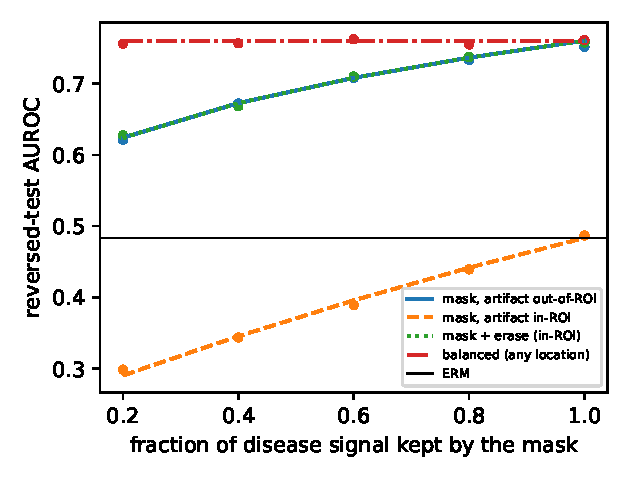
\includegraphics[width=0.6\linewidth]{../../paper/figures/theory.pdf}
\caption{Theory (lines) vs simulation (points).}\label{fig:theory}\end{figure}
\textbf{Conclusion.} Quantitatively close agreement, but by the pre-registered rule a ``qualitative account'' (one of 14
crossover signs disagrees at $-0.002$). The papers must not say the theory ``predicts'' magnitudes; they say it matches
held-out results. Its failure on chest drains marks its boundary (correlate-carried shortcuts are invisible in the clean
and correlated environments).

\section{Stage 9 --- remedies for frozen foundation-model features}
\textbf{Evolution of the method.} (1) \emph{Insert-then-erase (I2E)} in the pilot: insert artifact \emph{templates}
(rulers) into images, estimate the subspace of feature changes, erase it --- works in controlled sweeps but needs an
artifact model. (2) \emph{Mask-then-erase (MtE)}: estimate the subspace on \emph{masked} images so that erasure targets
exactly what masking leaves. (3) \emph{U-MtE}: replace templates by one \emph{generic} procedural overlay library (strokes,
bands, patches, blobs, dashed lines, glyphs; random colour/opacity/position, half centred in the ROI) used unchanged for
every modality; rank $k$ = smallest with 90\% held-out difference energy (cap 64); logistic head on erased masked features.
Needs no artifact example, artifact mask or artifact label --- only the ROI mask. (4) \emph{Disease protection}: erase
$\mathrm{orth}((I-WW^\top)U_k)$ with $W$ = label directions on artifact-free images. (5) \emph{U-MtE$_{\text{bal}}$}:
group-balanced head when image-level artifact labels exist. Registry \S\ref{doc:PREREGISTRATION_UNIVERSAL_I2E} (U1--U14).
\textbf{Main results.} Thyroid $+0.222$ [$+0.197,+0.251$] (DINOv2), $+0.204$ [$+0.174,+0.237$] (MedSigLIP), $+0.128$
[$+0.112,+0.145$] (ConvNeXt); ovary (MedSigLIP) $+0.215$ [$+0.182,+0.246$]; hair $+0.052$; controlled sweeps $+0.08$ to
$+0.28$. Real capsule: unprotected $-0.115$ (debris $\approx$ erosion fibrin), protected $-0.010$ (safety net; costs $\le0.012$
elsewhere). Erase vs augment with the same overlays (U7): thyroid $+0.207$, hair $+0.045$, ovary $+0.035$ (not robust to
embedding groups), capsule $-0.130$. With artifact labels, U-MtE$_{\text{bal}}$ is the most robust thyroid model
(min(rev,corr) 0.788 DINOv2, 0.792 MedSigLIP); mask+DFR best on capsule (0.885 vs 0.857); DFR best on hair (0.741).
The full arm $\times$ cohort table is Appendix Table \texttt{main\_inroi}.
\textbf{Rank ablation} (registry \S\ref{doc:PREREGISTRATION_UMTE_ABLATION}):
\begin{table}[H]\centering\scriptsize
\caption{U-MtE erasure-rank ablation (Trap A reversed AUROC, mean over seeds; e = held-out energy, k = fixed rank).}\label{tab:abl}
\begin{tabular}{llccccc}\toprule
Cohort & Rank rule & mask & U-MtE & U-MtE$_{\text{prot}}$ & U-MtE$-$mask & prot$-$mask \\\midrule
capsule & e0.50 & 0.684 & 0.630 & 0.676 & -0.054 & -0.008 \\
capsule & e0.90 & 0.684 & 0.569 & 0.673 & -0.115 & -0.010 \\
capsule & e0.99 & 0.684 & 0.569 & 0.673 & -0.115 & -0.010 \\
capsule & k1 & 0.684 & 0.685 & 0.685 & +0.001 & +0.001 \\
capsule & k16 & 0.684 & 0.634 & 0.675 & -0.050 & -0.009 \\
capsule & k4 & 0.684 & 0.676 & 0.681 & -0.008 & -0.002 \\
capsule & k64 & 0.684 & 0.569 & 0.673 & -0.115 & -0.010 \\
ovary & e0.50 & 0.545 & 0.543 & 0.578 & -0.002 & +0.033 \\
ovary & e0.90 & 0.545 & 0.564 & 0.588 & +0.019 & +0.043 \\
ovary & e0.99 & 0.545 & 0.564 & 0.588 & +0.019 & +0.043 \\
ovary & k1 & 0.545 & 0.558 & 0.552 & +0.012 & +0.007 \\
ovary & k16 & 0.545 & 0.535 & 0.565 & -0.010 & +0.020 \\
ovary & k4 & 0.545 & 0.504 & 0.560 & -0.041 & +0.015 \\
ovary & k64 & 0.545 & 0.564 & 0.588 & +0.019 & +0.043 \\
thyroid & e0.50 & 0.400 & 0.611 & 0.611 & +0.211 & +0.211 \\
thyroid & e0.90 & 0.400 & 0.622 & 0.617 & +0.222 & +0.217 \\
thyroid & e0.99 & 0.400 & 0.622 & 0.617 & +0.222 & +0.217 \\
thyroid & k1 & 0.400 & 0.471 & 0.451 & +0.071 & +0.051 \\
thyroid & k16 & 0.400 & 0.580 & 0.576 & +0.180 & +0.176 \\
thyroid & k4 & 0.400 & 0.463 & 0.451 & +0.063 & +0.051 \\
thyroid & k64 & 0.400 & 0.622 & 0.617 & +0.222 & +0.217 \\
\bottomrule\end{tabular}\end{table}

\textbf{Baselines and alternatives (each pre-registered).}
\begin{itemize}[leftmargin=*]\itemsep0pt
\item \textbf{JTT} (label-free): U-MtE beats it on thyroid ($+0.198$) and ovary ($+0.137$); JTT wins on hair.
\item \textbf{SPLINCE} (Holstege, Ravfogel \& Wouters, NeurIPS 2025; faithful whitened implementation): with artifact labels
it removes much disease signal (clean 0.56--0.78) and flips the shortcut on capsule; U-MtE$_{\text{bal}}$ more robust on
thyroid, capsule and hair (0.788 vs 0.596; 0.857 vs 0.683; 0.704 vs 0.564); on drains SPLINCE 0.516 vs 0.460.
\item \textbf{LEACE} (paired/unpaired): unpaired erasure with image-level labels flips the shortcut; paired recovers little.
\item \textbf{LaMa inpainting} with oracle artifact masks: strong; protected U-MtE matches it on thyroid without masks
($-0.009$ [$-0.045,+0.023$]), below it on ovary; U-MtE$_{\text{bal}}$ beats it.
\item \textbf{Text-prompted erasure} (biased prompts; MedSigLIP, DermLIP): near no-op ($\le+0.008$ over masking).
\item \textbf{SLAS} (few-shot patch-token suppression): localises hair from 5 annotated images (patch AUROC 0.93), small
classification gains ($+0.02$ hair, $+0.08$ thyroid).
\item \textbf{Pseudo-group balancing} (U8; overlay-detector pseudo labels): $+0.04$ on thyroid, none on hair.
\item \textbf{Erasure + DFR} (U10): no gain over masking + DFR.
\item \textbf{Validation-driven selectors} (U13, U14): beat masking in 5/5 cohorts ($+0.17$ to $+0.40$), within 0.02 of the
best candidate in 5/5, beat DFR in 3/5; split-validation variant fixes drains (0.656); neither uniformly best.
\end{itemize}

\section{Stage 10 --- end-to-end fine-tuning and remedies for fine-tuned networks}
\textbf{Design} (registry \S\ref{doc:PREREGISTRATION_FINETUNE}): ResNet-50 (ImageNet, 224\,px, 8 epochs, AdamW, lr
$10^{-4}$, head lr $\times10$, OneCycle, fp16) and ViT-S/16 (lr $3\cdot10^{-5}$); seed 42, folds 0--4 as bootstrap
clusters; thresholds on clean validation.
\textbf{Location law.} Capsule (ResNet-50): masking harms in-ROI ($-0.284$ [$-0.347,-0.226$]), helps out ($+0.301$),
crossover $+0.584$ [$+0.469,+0.691$]; thyroid ViT-S crossover $+0.168$ [$+0.074,+0.265$]; thyroid ResNet-50 $+0.057$
[$-0.021,+0.130$].
\textbf{Remedies tried for fine-tuned networks.}
\begin{itemize}[leftmargin=*]\itemsep0pt
\item \texttt{mte\_ft} (invariance penalty between masked images with and without a generic overlay): thyroid ResNet-50
$+0.143$ [$+0.099,+0.188$] \ok; ViT-S $+0.009$ \no; capsule $-0.021$ \no.
\item \texttt{mte\_post} (fine-tune like \texttt{mask}, then U-MtE on the penultimate features; registry
\S\ref{doc:PREREGISTRATION_FT_ERASE}): $+0.004$ [$+0.000,+0.012$] over the same features without erasure \no. After
unconstrained fine-tuning the caliper is encoded along task-specific directions that generic overlays do not move.
\item \texttt{umte\_ft} (erase-while-fine-tuning: running overlay-shift subspace projected out before the head at every
step, plus the invariance penalty; registry \S\ref{doc:PREREGISTRATION_FT_UMTE}): ResNet-50 $+0.160$ [$+0.114,+0.207$]
over masking and $+0.016$ over \texttt{mte\_ft}; ViT-S $+0.061$ [$-0.005,+0.141$] over masking, $+0.052$ [$+0.007,+0.107$]
over \texttt{mte\_ft} \mixed. Note: on ResNet-50 correlated AUROC (0.664) is slightly below reversed (0.695) --- mild
over-correction.
\item \texttt{cons\_ft} (prediction consistency between masked images with and without an overlay): ResNet-50 $+0.007$
[$-0.014,+0.029$] \no; ViT-S $+0.062$ [$+0.031,+0.087$] \ok.
\item \textbf{\texttt{umte\_cons\_ft} (all three combined; pre-registered amendment before running):} ResNet-50 $+0.157$
[$+0.114,+0.205$], ViT-S $+0.143$ [$+0.103,+0.187$] \ok\ --- the first remedy that works for fully fine-tuned networks of
both architecture families without artifact annotation. AUROC clean/corr/rev: ResNet-50 0.688/0.661/0.693 (mask
0.691/0.827/0.536; mild over-correction); ViT-S 0.712/0.798/0.608 (mask 0.688/0.868/0.465).
\item Other cohorts (ResNet-50): \texttt{umte\_ft} ovary $+0.107$ [$-0.003,+0.229$]; \texttt{umte\_cons\_ft} (Amendment 2; run after recovering the GPU with a private copy of the identical driver
library): ovary $+0.094$ [$-0.011,+0.210$] \mixed\ (better than masking on clean, correlated and reversed AUROC,
0.687/0.726/0.650 vs 0.578/0.570/0.556; underpowered cohort); capsule $-0.022$ [$-0.046,+0.001$] \no\ (pathology-like
debris; fine-tuned masking collapses to 0.211 and only label-based balancing helps, mask+balanced 0.687).
\end{itemize}
\begin{table}[H]\centering\scriptsize
\caption{Every end-to-end fine-tuning contrast (5 folds of seed 42 as clusters).}\label{tab:ft}
\begin{tabular}{lllll}\toprule
Cohort & Architecture & Trap & Contrast & $\Delta$ reversed AUROC [95\% CI] \\\midrule
capsule & ResNet-50 & trapA & mask $-$ erm & -0.284 [-0.347, -0.226] \\
capsule & ResNet-50 & trapA & mte\_ft $-$ mask & -0.021 [-0.039, -0.003] \\
capsule & ResNet-50 & trapA & mask\_balanced $-$ balanced & +0.017 [-0.070, +0.105] \\
capsule & ResNet-50 & trapA & mte\_ft $-$ erm & -0.305 [-0.367, -0.246] \\
capsule & ResNet-50 & trapB & mask $-$ erm & +0.301 [+0.225, +0.380] \\
capsule & ResNet-50 & trapB & mte\_ft $-$ mask & -0.205 [-0.286, -0.111] \\
capsule & ResNet-50 & trapB & mask\_balanced $-$ balanced & -0.024 [-0.117, +0.065] \\
capsule & ResNet-50 & trapB & mte\_ft $-$ erm & +0.096 [-0.003, +0.194] \\
ovary & ResNet-50 & trapA & mask $-$ erm & +0.098 [-0.001, +0.212] \\
ovary & ResNet-50 & trapA & mte\_ft $-$ mask & +0.094 [-0.025, +0.217] \\
ovary & ResNet-50 & trapA & mask\_balanced $-$ balanced & -0.009 [-0.128, +0.109] \\
ovary & ResNet-50 & trapA & mte\_ft $-$ erm & +0.192 [+0.103, +0.278] \\
ovary & ResNet-50 & trapA & umte\_ft $-$ mask & +0.107 [-0.003, +0.229] \\
ovary & ResNet-50 & trapA & umte\_ft $-$ mte\_ft & +0.013 [-0.049, +0.074] \\
ovary & ResNet-50 & trapB & mask $-$ erm & +0.234 [+0.084, +0.376] \\
ovary & ResNet-50 & trapB & mte\_ft $-$ mask & +0.014 [-0.067, +0.104] \\
ovary & ResNet-50 & trapB & mask\_balanced $-$ balanced & -0.007 [-0.128, +0.120] \\
ovary & ResNet-50 & trapB & mte\_ft $-$ erm & +0.248 [+0.123, +0.366] \\
thyroid & ResNet-50 & trapA & mask $-$ erm & +0.105 [+0.067, +0.141] \\
thyroid & ResNet-50 & trapA & mte\_ft $-$ mask & +0.143 [+0.099, +0.188] \\
thyroid & ResNet-50 & trapA & mask\_balanced $-$ balanced & +0.147 [+0.104, +0.192] \\
thyroid & ResNet-50 & trapA & mte\_ft $-$ erm & +0.248 [+0.209, +0.288] \\
thyroid & ResNet-50 & trapA & mte\_post $-$ mask & -0.027 [-0.053, -0.001] \\
thyroid & ResNet-50 & trapA & mte\_post $-$ mask\_post & +0.004 [+0.000, +0.012] \\
thyroid & ResNet-50 & trapA & umte\_ft $-$ mask & +0.160 [+0.114, +0.207] \\
thyroid & ResNet-50 & trapA & umte\_ft $-$ mte\_ft & +0.016 [+0.002, +0.030] \\
thyroid & ResNet-50 & trapA & cons\_ft $-$ mask & +0.007 [-0.014, +0.029] \\
thyroid & ResNet-50 & trapA & umte\_cons\_ft $-$ mask & +0.157 [+0.114, +0.205] \\
thyroid & ResNet-50 & trapB & mask $-$ erm & +0.161 [+0.096, +0.226] \\
thyroid & ResNet-50 & trapB & mte\_ft $-$ mask & -0.034 [-0.062, -0.008] \\
thyroid & ResNet-50 & trapB & mask\_balanced $-$ balanced & +0.123 [+0.061, +0.185] \\
thyroid & ResNet-50 & trapB & mte\_ft $-$ erm & +0.128 [+0.066, +0.192] \\
thyroid & ViT-S/16 & trapA & mask $-$ erm & +0.088 [+0.051, +0.126] \\
thyroid & ViT-S/16 & trapA & mte\_ft $-$ mask & +0.009 [-0.021, +0.040] \\
thyroid & ViT-S/16 & trapA & mask\_balanced $-$ balanced & +0.017 [-0.023, +0.055] \\
thyroid & ViT-S/16 & trapA & mte\_ft $-$ erm & +0.098 [+0.066, +0.129] \\
thyroid & ViT-S/16 & trapA & umte\_ft $-$ mask & +0.061 [-0.005, +0.141] \\
thyroid & ViT-S/16 & trapA & umte\_ft $-$ mte\_ft & +0.052 [+0.007, +0.107] \\
thyroid & ViT-S/16 & trapA & cons\_ft $-$ mask & +0.062 [+0.031, +0.087] \\
thyroid & ViT-S/16 & trapA & umte\_cons\_ft $-$ mask & +0.143 [+0.103, +0.187] \\
thyroid & ViT-S/16 & trapB & mask $-$ erm & +0.256 [+0.164, +0.354] \\
thyroid & ViT-S/16 & trapB & mte\_ft $-$ mask & -0.000 [-0.020, +0.019] \\
thyroid & ViT-S/16 & trapB & mask\_balanced $-$ balanced & +0.069 [+0.009, +0.141] \\
thyroid & ViT-S/16 & trapB & mte\_ft $-$ erm & +0.256 [+0.161, +0.358] \\
\bottomrule\end{tabular}\end{table}

\begin{table}[H]\centering\scriptsize
\caption{End-to-end fine-tuning: AUROC per arm (mean over folds).}\label{tab:ftauc}
\begin{tabular}{lllllccc}\toprule
Cohort & Arch. & Trap & Arm & Clean & Correlated & Reversed \\\midrule
isic & ResNet-50 & trapA & balanced & 0.766 & 0.838 & 0.696 \\
isic & ResNet-50 & trapA & erm & 0.730 & 0.905 & 0.532 \\
isic & ResNet-50 & trapA & mask & 0.733 & 0.896 & 0.530 \\
isic & ResNet-50 & trapA & mask\_balanced & 0.762 & 0.842 & 0.689 \\
isic & ResNet-50 & trapB & balanced & 0.720 & 0.755 & 0.733 \\
isic & ResNet-50 & trapB & erm & 0.687 & 0.867 & 0.489 \\
isic & ResNet-50 & trapB & mask & 0.708 & 0.777 & 0.630 \\
isic & ResNet-50 & trapB & mask\_balanced & 0.722 & 0.684 & 0.762 \\
ovary & ResNet-50\_power & trapA & erm & 0.596 & 0.708 & 0.464 \\
ovary & ResNet-50\_power & trapA & mask & 0.610 & 0.595 & 0.616 \\
ovary & ResNet-50\_power & trapB & erm & 0.500 & 0.658 & 0.362 \\
ovary & ResNet-50\_power & trapB & mask & 0.573 & 0.583 & 0.573 \\
ovary & ResNet-50\_power\_g4 & trapA & mask & 0.575 & 0.571 & 0.585 \\
ovary & ResNet-50\_power\_g4 & trapA & umte\_cons\_ft & 0.675 & 0.726 & 0.630 \\
\bottomrule\end{tabular}\end{table}


\section{Stage 11 --- robustness, leakage and integrity}\label{sec:robust}
\textbf{Artifact-label definitions} (registry \S\ref{doc:SENSITIVITY_ARTIFACT_LABELS}): large-marker ($\ge50$\,px) and
strict-location ($r\ge0.7$ / $r<0.05$) variants keep the crossover (thyroid $+0.215$ to $+0.262$; ovary $+0.170$ to $+0.195$)
and the protected-U-MtE gain (thyroid $+0.217$ to $+0.282$; ovary $+0.043$ to $+0.067$) significant; strict capsule Trap B
$+0.259$. \textbf{Mask audit} (registry \S\ref{doc:ARTIFACT_MASK_AUDIT}): 40 images per cell inspected.
\textbf{Leakage.} (i) Random vs grouped splits (Table~\ref{tab:leak}). (ii) Stricter embedding groups for the three cohorts
without patient IDs (registry \S\ref{doc:PREREGISTRATION_EMBEDDING_GROUPS}; amendment: embeddings mean-centred because raw
cosine was $\approx0.99$ for all ovary pairs):
\begin{table}[H]\centering\small
\caption{Embedding-based near-duplicate groups (mean-centred DINOv2 CLS, cosine $\ge\tau$).}\label{tab:embg}
\begin{tabular}{lccccc}\toprule
Cohort & Images & Groups (pHash/frames) & Groups (+embedding) & $\tau$ & Largest group share \\\midrule
thyroid & 3493 & 3455 & 3081 & 0.8 & 0.045805897509304326 \\
ovary & 1202 & 1059 & 969 & 0.8 & 0.020798668885191347 \\
capsule & 5481 & 137 & 135 & 0.93 & 0.03667214012041598 \\
\bottomrule\end{tabular}\end{table}

\begin{table}[H]\centering\scriptsize
\caption{Primary contrasts under stricter embedding-based leakage groups.}\label{tab:emb}
\begin{tabular}{llccc}\toprule
Cohort & Test & Main groups & Embedding groups & Robust \\\midrule
Thyroid & P1 location crossover & +0.230 [+0.204, +0.255] & +0.235 [+0.211, +0.259] & yes \\
Thyroid & P2 U-MtE (protected) > mask & +0.217 [+0.174, +0.257] & +0.251 [+0.219, +0.279] & yes \\
Thyroid & P3 erase > augment & +0.207 [+0.182, +0.235] & +0.192 [+0.162, +0.218] & yes \\
Thyroid & P4 U-MtE+balanced > balanced & +0.112 [+0.090, +0.134] & +0.152 [+0.138, +0.167] & yes \\
Ovary & P1 location crossover & +0.170 [+0.116, +0.224] & +0.157 [+0.080, +0.235] & yes \\
Ovary & P2 U-MtE (protected) > mask & +0.043 [+0.026, +0.061] & +0.047 [+0.020, +0.072] & yes \\
Ovary & P3 erase > augment & +0.035 [+0.010, +0.059] & +0.020 [-0.011, +0.053] & \textbf{no} \\
Ovary & P4 U-MtE+balanced > balanced & +0.028 [+0.000, +0.057] & +0.039 [+0.015, +0.064] & yes \\
Capsule & P1 location crossover & +0.368 [+0.340, +0.397] & +0.394 [+0.359, +0.430] & yes \\
Capsule & P2 U-MtE (protected) > mask & -0.010 [-0.021, -0.001] & -0.007 [-0.013, -0.001] & yes \\
Capsule & P3 erase > augment & -0.130 [-0.147, -0.110] & -0.136 [-0.153, -0.122] & yes \\
Capsule & P4 U-MtE+balanced > balanced & +0.082 [+0.064, +0.100] & +0.068 [+0.050, +0.085] & yes \\
\bottomrule\end{tabular}\end{table}

\textbf{Integrity.} Every CI in both papers is traced automatically to a result file (\texttt{scripts/verify/audit\_paper\_numbers.py};
109/109). All 146 result archives pass a gzip check after one regeneration (identical numbers). Deterministic arms were
verified identical across historical run folders. Deviations from pre-registrations are recorded in each document
(e.g.\ grid trimming in the rank ablation, fp32 features in fine-tune-then-erase, one skipped sweep in the theory test).

\section{Stage 12 --- datasets considered and not used}
CANDID-PTX (no access); CXR CLiP real devices (masking helps at both locations --- no in-ROI regime); CXR cardiomegaly lines
(too few labelled); TCGA/GrandQC pathology pen marks (unreliable masks); ISIC ink (70 in-lesion images); breast ultrasound
BUSI/BUS-BRA (two attempts: caliper labels $\approx$70\% pure; only 19/2{,}522 overlay-free images --- registry
\S\ref{doc:BREAST_MARKER_AUDIT}); EAD endoscopy (no disease labels); BKAI-IGH NeoPolyp colonoscopy (no specular-free images);
DINOv3 (weights gated, access refused).

\section{Cross-cutting methods}
\begin{itemize}[leftmargin=*]\itemsep1pt
\item \textbf{Backbones.} DINOv2 ViT-S/B/L-14 @518 (CLS), MedSigLIP-448 (image features, joint space), DermLIP/PanDerm (512-d
joint space), RAD-DINO @518, ConvNeXt-Base @384; fine-tuned ResNet-50 and ViT-S/16. Views rendered at 518\,px; features
cached per view (\texttt{erm}, \texttt{mask}, \texttt{mask\_insert\_generic}, \ldots).
\item \textbf{Heads.} Logistic regression; $C$ and the decision threshold (balanced accuracy) chosen on clean validation only.
\item \textbf{Seeds.} Real traps: 42, 123, 456, 789, 2026 $\times$ 5 folds; controlled sweeps: 42, 123, 456; fine-tuning:
seed 42, folds 0--4; natural tests: 5 seeds; bootstrap seeds deterministic per comparison (string hash).
\item \textbf{Statistics.} Hierarchical paired bootstrap (10{,}000); two-sided bootstrap $p$; Holm over the 16 primary tests.
\item \textbf{Compute.} One RTX 3090 (24 GB), 8 CPU cores, 31 GB RAM; about two days end to end.
\item \textbf{Reproduction.} \texttt{make data data\_extra verify synthetic isic2019 thyroid ovary capsule cxr drain natural
finetune sensitivity scale lama baselines analysis paper}; tool: \texttt{python -m wtss.umte}, \texttt{python -m wtss.slas}.
\end{itemize}

\section{External review and responses}\label{sec:review}
\begin{enumerate}[leftmargin=*]\itemsep1pt
\item ``U-MtE needs no mask'' is misleading (it uses the ROI mask) --- \emph{valid}; wording fixed everywhere.
\item Table 1 calls the method I2E --- \emph{valid}; renamed ``insert-then-erase (artifact templates)'' and explained.
\item GroupDRO claimed as benchmarked --- \emph{partly valid}; now scoped to the controlled dermoscopy sweeps.
\item Title omits X-ray --- \emph{valid, minor}; chest radiography named as a boundary case.
\item Patient/video leakage in TN3K/SEE-AI --- \emph{valid}; embedding-group sensitivity added (11/12 robust).
\item Theory only checked against its own simulation --- \emph{valid}; real-encoder test added (r = 0.997).
\item End-to-end evidence weaker --- \emph{valid}; U-MtE framed for frozen features; post-hoc and erase-while-fine-tuning tested.
\item Clinical metrics missing --- \emph{valid}; AUPRC, Brier, ECE, sensitivity/specificity added.
\item Related work thin --- \emph{valid}; six verified references added (Pewton 2024, Wang 2024, Germani 2026 MedIA, Lin
2024 MICCAI, Zech 2018, Brown 2023).
\end{enumerate}

\section{Conclusions and guidance for writing the paper}
\textbf{Claims the evidence supports (safe to make).}
\begin{enumerate}[leftmargin=*]\itemsep1pt
\item ROI masking helps much less for in-ROI than out-of-ROI artifacts (4/4 real cohorts, Holm; all replications).
\item In-ROI masking can be harmful, including on unaltered data and in clinical metrics (thyroid sensitivity).
\item The mechanism is retention with amplified reliance (counterfactual sensitivity, dilation, lesion-size strata).
\item A two-parameter linear-Gaussian account reproduces all signs and closely matches held-out results of real encoders;
call it a qualitative account.
\item For frozen foundation-model features, U-MtE removes in-ROI shortcuts carried by distinct overlays (thyroid across
3 families $\times$ 3 sizes; ovary with MedSigLIP) without artifact annotation; erasure beats augmentation (thyroid, hair);
protection makes it safe for pathology-like artifacts; text-prompted erasure does not work.
\item What carries the shortcut decides the method: pixels (U-MtE), pathology-like appearance (protected U-MtE or
mask+DFR), correlates (DFR/balancing).
\end{enumerate}
\textbf{Claims to avoid.} ``Masking always harms in-ROI'' (it helps a little on real thyroid/ovary/capsule); ``the
theory predicts magnitudes''; ``U-MtE works post hoc on fine-tuned networks'' (null); ``erase-while-fine-tuning works for any architecture and
disease'' (shown for ResNet-50 and ViT-S on thyroid; see Stage 10 for other cohorts); ``erase beats augment in ovary'' (not robust); ``four diseases and four
modalities'' (chest radiography is a boundary case); any claim of patient-level independence for TN3K, MMOTU, SEE-AI.
\textbf{Limitations.} Detector-based artifact labels (audited); no patient IDs for three cohorts; reversed environments are
constructed by subsampling; disease protection needs diagnosis labels of artifact-free images; balanced variants need
image-level artifact labels; the theory is fitted per model and blind to correlate-carried shortcuts.
\textbf{Suggested paper structure} (as in \texttt{paper\_neurips/main.tex}): teaser with real images; location-law table;
theory with the real-encoder figure; natural-data table; compact remedies table; forest plot; mechanism and dose-response
figures in the appendix; scale, leakage, clinical metrics and fine-tuning in the robustness appendix.

\appendix
\part{Appendices}
\section{All generated paper tables}\label{app:tables}
{\small\subsection*{main inroi}
\begin{table*}[t]\centering\scriptsize
\caption{In-ROI artifacts (Trap~A): reversed-test AUROC, with min(reversed, correlated) in parentheses (penalises shortcut flipping). Best robust value per column in bold. Generated by \texttt{scripts/make\_main\_table.py}.}
\label{tab:main}
\begin{tabular}{llcccccccccc}
\toprule
Method & Needs & \rotatebox{90}{Hair/DINOv2} & \rotatebox{90}{Hair/DermLIP} & \rotatebox{90}{Thyroid/DINOv2} & \rotatebox{90}{Thyroid/MedSigLIP} & \rotatebox{90}{Thyroid/ConvNeXt} & \rotatebox{90}{Capsule/DINOv2} & \rotatebox{90}{Capsule/MedSigLIP} & \rotatebox{90}{Capsule/ConvNeXt} & \rotatebox{90}{Drain/RAD-DINO} & \rotatebox{90}{Drain/DINOv2} \\
\midrule
ERM & — & 0.49 (0.49) & 0.67 (0.67) & 0.29 (0.29) & 0.28 (0.28) & 0.35 (0.35) & 0.59 (0.59) & 0.59 (0.59) & 0.55 (0.55) & 0.19 (0.19) & 0.28 (0.28) \\
ROI masking & ROI & 0.45 (0.45) & 0.58 (0.58) & 0.40 (0.40) & 0.35 (0.35) & 0.36 (0.36) & 0.68 (0.68) & 0.70 (0.70) & 0.64 (0.64) & 0.24 (0.24) & 0.29 (0.29) \\
Mask + overlay augmentation & ROI & 0.46 (0.46) & – & 0.42 (0.42) & 0.38 (0.38) & 0.37 (0.37) & 0.70 (0.70) & 0.72 (0.72) & 0.65 (0.65) & 0.24 (0.24) & 0.29 (0.29) \\
\textbf{U-MtE (ours)} & ROI & 0.51 (0.51) & 0.51 (0.51) & 0.62 (0.62) & 0.55 (0.55) & 0.49 (0.49) & 0.57 (0.57) & 0.47 (0.47) & 0.56 (0.56) & 0.27 (0.27) & 0.28 (0.28) \\
\textbf{U-MtE, protected (ours)} & ROI + $Y$ of $A{=}0$ & 0.49 (0.49) & 0.59 (0.59) & 0.62 (0.62) & 0.61 (0.61) & 0.55 (0.55) & 0.67 (0.67) & 0.67 (0.67) & 0.64 (0.64) & 0.27 (0.27) & 0.28 (0.28) \\
Group-balanced & $A$ & 0.72 (0.72) & \textbf{0.81 (0.81)} & 0.68 (0.68) & 0.70 (0.70) & 0.66 (0.66) & 0.78 (0.78) & 0.81 (0.81) & 0.72 (0.72) & 0.54 (0.54) & 0.40 (0.40) \\
DFR & $A$ & \textbf{0.74 (0.74)} & 0.78 (0.78) & 0.74 (0.66) & 0.76 (0.72) & 0.71 (0.67) & 0.80 (0.80) & 0.80 (0.80) & 0.77 (0.77) & \textbf{0.68 (0.68)} & 0.55 (0.55) \\
Mask + DFR & ROI + $A$ & 0.69 (0.69) & – & 0.83 (0.74) & 0.81 (0.76) & 0.77 (0.72) & \textbf{0.88 (0.88)} & \textbf{0.90 (0.90)} & \textbf{0.86 (0.86)} & 0.65 (0.65) & \textbf{0.57 (0.57)} \\
\textbf{U-MtE + balanced (ours)} & ROI + $A$ & 0.70 (0.70) & 0.65 (0.65) & \textbf{0.79 (0.79)} & \textbf{0.79 (0.79)} & \textbf{0.74 (0.74)} & 0.86 (0.86) & 0.85 (0.85) & 0.80 (0.80) & 0.46 (0.46) & 0.44 (0.44) \\
\bottomrule
\end{tabular}
\end{table*}

\clearpage
\subsection*{main inroi compact}
\begin{table}[t]\centering\small
\caption{In-ROI artifacts (Trap~A): robustness $=\min(\text{reversed},\text{correlated})$ AUROC, which penalises both shortcut use and shortcut flipping. Bold: best per column. Full reversed/correlated/clean values for all cohorts and backbones: Supplement~S8.}
\label{m:tab:remedies}
\begin{tabular}{llccccc}
\toprule
Method & Needs & \shortstack{Hair\\ \scriptsize DINOv2} & \shortstack{Thyroid\\ \scriptsize DINOv2} & \shortstack{Thyroid\\ \scriptsize MedSigLIP} & \shortstack{Ovary\\ \scriptsize DINOv2} & \shortstack{Capsule\\ \scriptsize DINOv2} \\
\midrule
ROI masking & ROI & 0.46 & 0.40 & 0.34 & 0.55 & 0.67 \\
Mask + overlay augmentation & ROI & 0.47 & 0.41 & 0.36 & 0.53 & 0.68 \\
U-MtE (ours) & ROI & 0.50 & 0.62 & 0.59 & 0.56 & 0.54 \\
U-MtE, protected (ours) & ROI & 0.50 & 0.68 & 0.65 & 0.59 & 0.66 \\
Group-balanced & $A$ & \textbf{0.72} & 0.68 & 0.70 & 0.70 & 0.76 \\
DFR & $A$ & 0.71 & 0.67 & 0.72 & 0.69 & 0.82 \\
Mask + DFR & ROI + $A$ & 0.66 & 0.75 & 0.77 & \textbf{0.75} & \textbf{0.89} \\
U-MtE + balanced (ours) & ROI + $A$ & 0.69 & \textbf{0.79} & \textbf{0.79} & 0.73 & 0.84 \\
\bottomrule
\end{tabular}
\end{table}

\clearpage
\subsection*{natural clinical}
\begin{table}[t]\centering\scriptsize
\caption{Clinical secondary metrics on the unaltered test sets (Table~\ref{m:tab:natural}): mean (SD) over training seeds. Sensitivity and specificity at the operating point fixed on clean validation data; ECE with 10 equal-width bins; AUPRC baseline = prevalence.}\label{tab:natural_clinical}
\begin{tabular}{llcccccc}\toprule
Test set & Arm & AUROC & AUPRC & Brier & ECE & Sens & Spec \\\midrule
Thyroid (official split) ($\pi=0.38$) & ERM & 0.736 (0.009) & 0.606 (0.012) & 0.207 (0.005) & 0.082 (0.008) & 0.734 (0.047) & 0.619 (0.061) \\
 & mask & 0.731 (0.006) & 0.632 (0.007) & 0.214 (0.006) & 0.120 (0.026) & 0.347 (0.095) & 0.888 (0.041) \\
 & U-MtE & 0.742 (0.003) & 0.638 (0.007) & 0.203 (0.001) & 0.085 (0.007) & 0.425 (0.088) & 0.854 (0.050) \\
 & balanced & 0.716 (0.007) & 0.584 (0.012) & 0.219 (0.004) & 0.110 (0.007) & 0.714 (0.052) & 0.599 (0.061) \\
 & U-MtE$_{\text{bal}}$ & 0.731 (0.004) & 0.630 (0.007) & 0.207 (0.001) & 0.084 (0.006) & 0.399 (0.069) & 0.866 (0.034) \\
\midrule
ISIC, BCN held out ($\pi=0.23$) & ERM & 0.786 (0.003) & 0.586 (0.003) & 0.239 (0.006) & 0.279 (0.011) & 0.842 (0.038) & 0.519 (0.075) \\
 & mask & 0.769 (0.004) & 0.571 (0.009) & 0.286 (0.007) & 0.332 (0.009) & 0.860 (0.013) & 0.439 (0.023) \\
 & U-MtE & 0.773 (0.004) & 0.574 (0.008) & 0.280 (0.009) & 0.328 (0.012) & 0.858 (0.039) & 0.448 (0.089) \\
 & balanced & 0.781 (0.005) & 0.585 (0.009) & 0.228 (0.006) & 0.257 (0.011) & 0.811 (0.046) & 0.554 (0.087) \\
 & U-MtE$_{\text{bal}}$ & 0.774 (0.004) & 0.568 (0.008) & 0.279 (0.011) & 0.325 (0.016) & 0.860 (0.027) & 0.447 (0.051) \\
\midrule
ISIC, MSK held out ($\pi=0.19$) & ERM & 0.770 (0.008) & 0.477 (0.012) & 0.172 (0.007) & 0.161 (0.019) & 0.608 (0.049) & 0.786 (0.039) \\
 & mask & 0.790 (0.004) & 0.512 (0.009) & 0.146 (0.003) & 0.115 (0.009) & 0.593 (0.052) & 0.824 (0.037) \\
 & U-MtE & 0.783 (0.004) & 0.500 (0.008) & 0.150 (0.003) & 0.126 (0.009) & 0.566 (0.073) & 0.831 (0.049) \\
 & balanced & 0.766 (0.008) & 0.462 (0.014) & 0.178 (0.008) & 0.170 (0.020) & 0.626 (0.047) & 0.755 (0.046) \\
 & U-MtE$_{\text{bal}}$ & 0.774 (0.006) & 0.482 (0.009) & 0.154 (0.004) & 0.131 (0.010) & 0.594 (0.061) & 0.798 (0.051) \\
\midrule
ISIC, HAM held out ($\pi=0.11$) & ERM & 0.750 (0.005) & 0.353 (0.005) & 0.162 (0.006) & 0.234 (0.011) & 0.535 (0.092) & 0.813 (0.068) \\
 & mask & 0.789 (0.002) & 0.404 (0.006) & 0.143 (0.005) & 0.217 (0.011) & 0.559 (0.112) & 0.842 (0.063) \\
 & U-MtE & 0.799 (0.008) & 0.406 (0.009) & 0.145 (0.007) & 0.226 (0.016) & 0.573 (0.067) & 0.846 (0.041) \\
 & balanced & 0.747 (0.017) & 0.346 (0.019) & 0.156 (0.014) & 0.228 (0.015) & 0.539 (0.078) & 0.803 (0.076) \\
 & U-MtE$_{\text{bal}}$ & 0.802 (0.005) & 0.401 (0.009) & 0.139 (0.006) & 0.215 (0.021) & 0.606 (0.054) & 0.825 (0.037) \\
\midrule
Capsule (held-out frames) ($\pi=0.56$) & ERM & 0.889 (0.019) & 0.897 (0.046) & 0.130 (0.016) & 0.042 (0.011) & 0.770 (0.062) & 0.844 (0.055) \\
 & mask & 0.967 (0.011) & 0.971 (0.014) & 0.069 (0.013) & 0.029 (0.011) & 0.859 (0.032) & 0.933 (0.025) \\
 & U-MtE & 0.962 (0.009) & 0.967 (0.013) & 0.081 (0.017) & 0.065 (0.045) & 0.871 (0.042) & 0.897 (0.043) \\
 & balanced & 0.881 (0.024) & 0.889 (0.053) & 0.136 (0.017) & 0.051 (0.009) & 0.758 (0.087) & 0.838 (0.059) \\
 & U-MtE$_{\text{bal}}$ & 0.959 (0.008) & 0.964 (0.012) & 0.079 (0.007) & 0.044 (0.012) & 0.866 (0.048) & 0.897 (0.052) \\
\bottomrule
\end{tabular}\end{table}

\clearpage
\subsection*{synthetic cxr raddino518}
\begin{table*}\scriptsize
\caption{Synthetic tube, NIH ChestX-ray14 pneumothorax, RAD-DINO @518}
\label{tab:synthetic_cxr_raddino518}
\resizebox{\textwidth}{!}{\begin{tabular}{lllllllllll}
\toprule
Method & Needs & clean@0 & rev@0 & clean@50 & rev@50 & clean@100 & rev@100 & Δrev@0 & Δrev@50 & Δrev@100 \\
\midrule
ERM & — & 0.915 & 0.913 & 0.911 & 0.772 & 0.907 & 0.614 &  &  &  \\
ROI masking & ROI mask (train+test) & 0.910 & 0.910 & 0.908 & 0.843 & 0.905 & 0.725 & -0.002 [-0.007, +0.002] & +0.070 [+0.062, +0.078] & +0.110 [+0.101, +0.120] \\
Inpainting (oracle) & artifact pixels (train+test) & 0.915 & 0.915 & 0.916 & 0.913 & 0.916 & 0.914 & +0.003 [+0.002, +0.003] & +0.140 [+0.127, +0.153] & +0.299 [+0.280, +0.321] \\
Group-balanced & image-level A (train) & 0.914 & 0.913 & 0.913 & 0.920 & 0.912 & 0.924 & +0.000 [-0.003, +0.003] & +0.147 [+0.134, +0.161] & +0.309 [+0.289, +0.330] \\
DFR & image-level A (val) & 0.900 & 0.898 & 0.899 & 0.889 & 0.897 & 0.894 & -0.014 [-0.019, -0.010] & +0.116 [+0.105, +0.128] & +0.280 [+0.256, +0.306] \\
LEACE (paired, oracle renders) & paired renders (train) & 0.916 & 0.915 & 0.914 & 0.912 & 0.908 & 0.901 & +0.003 [+0.002, +0.003] & +0.139 [+0.127, +0.153] & +0.287 [+0.266, +0.309] \\
Insert-then-erase (artifact templates) & artifact templates & 0.911 & 0.910 & 0.908 & 0.907 & 0.906 & 0.905 & -0.002 [-0.006, +0.001] & +0.135 [+0.122, +0.149] & +0.291 [+0.271, +0.312] \\
Insert-then-erase + balanced (artifact templates) & artifact templates + A (train) & 0.907 & 0.907 & 0.907 & 0.907 & 0.907 & 0.907 & -0.006 [-0.010, -0.001] & +0.134 [+0.120, +0.150] & +0.292 [+0.270, +0.316] \\
Insert-then-erase rank-1 (ablation) & artifact templates & 0.915 & 0.915 & 0.914 & 0.910 & 0.910 & 0.867 & +0.002 [+0.001, +0.003] & +0.138 [+0.125, +0.151] & +0.253 [+0.235, +0.271] \\
Insertion augmentation & artifact templates & 0.915 & 0.915 & 0.913 & 0.856 & 0.911 & 0.726 & +0.002 [+0.001, +0.003] & +0.084 [+0.074, +0.093] & +0.112 [+0.098, +0.125] \\
\bottomrule
\end{tabular}}
\end{table*}

\clearpage
\subsection*{synthetic interaction}
\begin{table*}\scriptsize
\caption{Location interaction [Δ vs ERM]\_0\% − [Δ vs ERM]\_100\% (DINOv2 @518)}
\label{tab:synthetic_interaction}
\resizebox{\textwidth}{!}{\begin{tabular}{ll}
\toprule
Method & Interaction (0\% − 100\%) \\
\midrule
ROI masking & +0.313 [+0.258, +0.370] \\
Inpainting (oracle) & -0.103 [-0.127, -0.080] \\
Group-balanced & -0.143 [-0.171, -0.119] \\
GroupDRO & -0.116 [-0.138, -0.096] \\
DFR & -0.154 [-0.178, -0.132] \\
LEACE (paired, oracle renders) & -0.127 [-0.158, -0.093] \\
Repair consistency & +0.002 [-0.024, +0.030] \\
Repair consistency, λ=0 & -0.010 [-0.036, +0.016] \\
\bottomrule
\end{tabular}}
\end{table*}

\clearpage
\subsection*{synthetic isic dermlip224}
\begin{table*}\scriptsize
\caption{Synthetic ruler, ISIC 2018, DermLIP/PanDerm @224}
\label{tab:synthetic_isic_dermlip224}
\resizebox{\textwidth}{!}{\begin{tabular}{lllllllllll}
\toprule
Method & Needs & clean@0 & rev@0 & clean@50 & rev@50 & clean@100 & rev@100 & Δrev@0 & Δrev@50 & Δrev@100 \\
\midrule
ERM & — & 0.932 & 0.697 & 0.930 & 0.624 & 0.932 & 0.574 &  &  &  \\
ROI masking & ROI mask (train+test) & 0.858 & 0.858 & 0.818 & 0.342 & 0.823 & 0.311 & +0.161 [+0.121, +0.202] & -0.282 [-0.343, -0.227] & -0.263 [-0.328, -0.195] \\
Group-balanced & image-level A (train) & 0.948 & 0.920 & 0.947 & 0.915 & 0.948 & 0.914 & +0.223 [+0.193, +0.252] & +0.291 [+0.243, +0.342] & +0.339 [+0.294, +0.391] \\
DFR & image-level A (val) & 0.946 & 0.934 & 0.944 & 0.922 & 0.943 & 0.923 & +0.237 [+0.200, +0.278] & +0.298 [+0.247, +0.362] & +0.348 [+0.310, +0.386] \\
LEACE (paired, oracle renders) & paired renders (train) & 0.951 & 0.946 & 0.950 & 0.942 & 0.954 & 0.938 & +0.249 [+0.214, +0.288] & +0.318 [+0.262, +0.378] & +0.364 [+0.318, +0.415] \\
I2E (ours) & template library & 0.915 & 0.879 & 0.917 & 0.847 & 0.921 & 0.826 & +0.183 [+0.147, +0.220] & +0.223 [+0.171, +0.282] & +0.251 [+0.205, +0.300] \\
I2E + balanced (ours) & templates + A (train) & 0.918 & 0.911 & 0.918 & 0.905 & 0.922 & 0.900 & +0.214 [+0.181, +0.248] & +0.281 [+0.233, +0.332] & +0.325 [+0.269, +0.384] \\
\bottomrule
\end{tabular}}
\end{table*}

\clearpage
\subsection*{synthetic isic dino224}
\begin{table*}\scriptsize
\caption{Synthetic ruler, ISIC 2018, DINOv2 @224}
\label{tab:synthetic_isic_dino224}
\resizebox{\textwidth}{!}{\begin{tabular}{lllllllllll}
\toprule
Method & Needs & clean@0 & rev@0 & clean@50 & rev@50 & clean@100 & rev@100 & Δrev@0 & Δrev@50 & Δrev@100 \\
\midrule
ERM & — & 0.794 & 0.438 & 0.797 & 0.410 & 0.800 & 0.391 &  &  &  \\
ROI masking & ROI mask (train+test) & 0.798 & 0.798 & 0.771 & 0.329 & 0.762 & 0.295 & +0.361 [+0.308, +0.413] & -0.081 [-0.119, -0.043] & -0.095 [-0.131, -0.059] \\
Group-balanced & image-level A (train) & 0.803 & 0.732 & 0.805 & 0.709 & 0.808 & 0.708 & +0.294 [+0.264, +0.328] & +0.299 [+0.271, +0.327] & +0.318 [+0.288, +0.347] \\
DFR & image-level A (val) & 0.737 & 0.729 & 0.741 & 0.734 & 0.740 & 0.726 & +0.291 [+0.229, +0.357] & +0.324 [+0.258, +0.396] & +0.335 [+0.269, +0.405] \\
LEACE (paired, oracle renders) & paired renders (train) & 0.830 & 0.830 & 0.829 & 0.824 & 0.826 & 0.816 & +0.392 [+0.351, +0.434] & +0.415 [+0.373, +0.456] & +0.426 [+0.383, +0.469] \\
Insert-then-erase (artifact templates) & artifact templates & 0.813 & 0.795 & 0.810 & 0.785 & 0.805 & 0.769 & +0.357 [+0.315, +0.400] & +0.375 [+0.334, +0.418] & +0.378 [+0.336, +0.419] \\
Insert-then-erase + balanced (artifact templates) & artifact templates + A (train) & 0.811 & 0.811 & 0.809 & 0.808 & 0.807 & 0.805 & +0.373 [+0.337, +0.410] & +0.398 [+0.360, +0.437] & +0.414 [+0.376, +0.452] \\
\bottomrule
\end{tabular}}
\end{table*}

\clearpage
\subsection*{synthetic isic dino518}
\begin{table}
\caption{Synthetic ruler, ISIC 2018, DINOv2 ViT-B/14 @518: AUROC and reversed-test Δ vs ERM [95% CI]}
\label{tab:synthetic_isic_dino518}
\begin{tabular}{lllllllllll}
\toprule
Method & Needs & clean@0 & rev@0 & clean@50 & rev@50 & clean@100 & rev@100 & Δrev@0 & Δrev@50 & Δrev@100 \\
\midrule
ERM & — & 0.797 & 0.665 & 0.793 & 0.573 & 0.792 & 0.515 &  &  &  \\
ROI masking & ROI mask (train+test) & 0.849 & 0.849 & 0.829 & 0.476 & 0.825 & 0.386 & +0.184 [+0.146, +0.224] & -0.097 [-0.138, -0.056] & -0.129 [-0.170, -0.087] \\
Inpainting (oracle) & artifact pixels (train+test) & 0.810 & 0.806 & 0.809 & 0.783 & 0.807 & 0.759 & +0.141 [+0.120, +0.162] & +0.211 [+0.187, +0.234] & +0.243 [+0.218, +0.269] \\
Group-balanced & image-level A (train) & 0.814 & 0.802 & 0.815 & 0.792 & 0.806 & 0.796 & +0.137 [+0.109, +0.168] & +0.219 [+0.188, +0.252] & +0.281 [+0.248, +0.315] \\
DFR & image-level A (val) & 0.786 & 0.789 & 0.787 & 0.794 & 0.789 & 0.794 & +0.124 [+0.091, +0.160] & +0.221 [+0.184, +0.261] & +0.279 [+0.240, +0.320] \\
LEACE (paired, oracle renders) & paired renders (train) & 0.829 & 0.832 & 0.810 & 0.810 & 0.809 & 0.809 & +0.167 [+0.139, +0.197] & +0.237 [+0.212, +0.263] & +0.294 [+0.265, +0.325] \\
Repair consistency & artifact pixels (train) & 0.828 & 0.707 & 0.822 & 0.616 & 0.814 & 0.558 & +0.042 [+0.015, +0.069] & +0.043 [+0.014, +0.072] & +0.042 [+0.012, +0.073] \\
I2E (ours) & template library & 0.848 & 0.844 & 0.850 & 0.833 & 0.847 & 0.818 & +0.179 [+0.152, +0.206] & +0.260 [+0.229, +0.291] & +0.303 [+0.271, +0.336] \\
I2E + balanced (ours) & templates + A (train) & 0.841 & 0.842 & 0.843 & 0.840 & 0.844 & 0.842 & +0.177 [+0.151, +0.205] & +0.267 [+0.238, +0.298] & +0.327 [+0.293, +0.362] \\
I2E rank-1 (ablation) & template library & 0.811 & 0.799 & 0.809 & 0.770 & 0.806 & 0.730 & +0.134 [+0.115, +0.154] & +0.197 [+0.174, +0.220] & +0.215 [+0.190, +0.240] \\
Insertion augmentation & template library & 0.814 & 0.726 & 0.812 & 0.654 & 0.810 & 0.603 & +0.061 [+0.049, +0.074] & +0.081 [+0.068, +0.094] & +0.088 [+0.077, +0.099] \\
\bottomrule
\end{tabular}
\end{table}

\clearpage
\subsection*{traps isic2019 dino518}
\begin{table*}\scriptsize
\caption{ISIC 2019 real hair, DINOv2 @518: Trap A (in-lesion) and Trap B (extra-lesional)}
\label{tab:traps_isic2019_dino518}
\resizebox{\textwidth}{!}{\begin{tabular}{llllllllllll}
\toprule
Method & Needs & A clean & A corr & A rev & B clean & B corr & B rev & A Δrev & A Δclean & B Δrev & B Δclean \\
\midrule
ERM & — & 0.753 & 0.925 & 0.389 & 0.760 & 0.925 & 0.359 &  &  &  &  \\
ROI masking & ROI mask (train+test) & 0.755 & 0.925 & 0.401 & 0.746 & 0.846 & 0.537 & +0.012 [-0.042, +0.062] & +0.002 & +0.178 [+0.142, +0.214] & -0.014 \\
Inpainting (oracle) & artifact pixels (train+test) & 0.753 & 0.896 & 0.559 & 0.750 & 0.882 & 0.478 & +0.171 [+0.132, +0.210] & -0.000 & +0.119 [+0.094, +0.141] & -0.010 \\
Group-balanced & image-level A (train) & 0.771 & 0.850 & 0.723 & 0.768 & 0.781 & 0.734 & +0.335 [+0.269, +0.400] & +0.018 & +0.375 [+0.332, +0.423] & +0.008 \\
DFR & image-level A (val) & 0.777 & 0.782 & 0.794 & 0.782 & 0.719 & 0.815 & +0.405 [+0.322, +0.484] & +0.024 & +0.456 [+0.396, +0.513] & +0.022 \\
LEACE (paired, removal) & artifact pixels (train) & 0.754 & 0.918 & 0.504 & 0.751 & 0.907 & 0.453 & +0.116 [+0.079, +0.156] & +0.001 & +0.094 [+0.074, +0.113] & -0.009 \\
LEACE (unpaired labels) & image-level A (train) & 0.761 & 0.639 & 0.869 & 0.754 & 0.615 & 0.833 & +0.480 [+0.414, +0.534] & +0.007 & +0.474 [+0.430, +0.516] & -0.006 \\
Insert-then-erase (artifact templates) & artifact templates & 0.745 & 0.926 & 0.456 & 0.751 & 0.919 & 0.406 & +0.067 [+0.035, +0.100] & -0.008 & +0.047 [+0.027, +0.068] & -0.009 \\
Insert-then-erase + balanced (artifact templates) & artifact templates + A (train) & 0.755 & 0.855 & 0.703 & 0.788 & 0.832 & 0.706 & +0.314 [+0.257, +0.366] & +0.002 & +0.347 [+0.308, +0.391] & +0.028 \\
Insert-then-erase rank-1 (ablation) & artifact templates & 0.753 & 0.926 & 0.389 & 0.757 & 0.925 & 0.358 & +0.001 [-0.002, +0.003] & -0.000 & -0.001 [-0.005, +0.002] & -0.003 \\
Insertion augmentation & artifact templates & 0.754 & 0.926 & 0.415 & 0.760 & 0.924 & 0.373 & +0.026 [+0.016, +0.037] & +0.001 & +0.014 [+0.005, +0.022] & +0.000 \\
Prevalence calibration & image-level A (train+test) & 0.753 & 0.468 & 0.900 & 0.760 & 0.488 & 0.887 & +0.511 [+0.456, +0.572] & +0.000 & +0.528 [+0.495, +0.560] & +0.000 \\
\bottomrule
\end{tabular}}
\end{table*}

\clearpage
\subsection*{traps isic2019 dino518 crossover}
\begin{table*}\scriptsize
\caption{ISIC 2019 real hair, DINOv2 @518: Trap A (in-lesion) and Trap B (extra-lesional) — location crossover [Δ vs ERM]\_TrapB − [Δ vs ERM]\_TrapA}
\label{tab:traps_isic2019_dino518_crossover}
\resizebox{\textwidth}{!}{\begin{tabular}{ll}
\toprule
Method & Crossover (B − A) \\
\midrule
Prevalence calibration & +0.017 [-0.046, +0.072] \\
ROI masking & +0.166 [+0.116, +0.215] \\
Inpainting (oracle) & -0.052 [-0.096, -0.016] \\
Group-balanced & +0.040 [-0.024, +0.109] \\
DFR & +0.051 [-0.008, +0.115] \\
LEACE (paired, removal) & -0.022 [-0.069, +0.013] \\
LEACE (unpaired labels) & -0.007 [-0.053, +0.042] \\
I2E (ours) & -0.020 [-0.051, +0.011] \\
I2E + balanced (ours) & +0.033 [-0.028, +0.090] \\
I2E rank-1 (ablation) & -0.002 [-0.006, +0.003] \\
Insertion augmentation & -0.012 [-0.029, +0.004] \\
\bottomrule
\end{tabular}}
\end{table*}

\clearpage}
\section{Result ledgers}\label{app:resultsmd}
\section{Pilot replication: all 88 numbers}
\noindent\textit{Source: results/SUMMARY.md}

{\small
Rule: MATCH = same sign, same CI-excludes-0 verdict, \textbar Δ\textbar{} ≤ 0.02; SIGN+CI = sign and CI verdict match, \textbar Δ\textbar{} \textgreater{} 0.02; MISMATCH otherwise.

Verdict counts: \{\textquotesingle MATCH\textquotesingle: 73, \textquotesingle SIGN+CI\textquotesingle: 12, \textquotesingle MISMATCH\textquotesingle: 3\}

{ % do not increment counter
\begin{longtable}[]{@{}llllll@{}}
\toprule\noalign{}
E & quantity & expected & obtained & verdict & source \\
\midrule\noalign{}
\endhead
\bottomrule\noalign{}
\endlastfoot
E1 & mask − ERM rev @0\% & +0.184 {[}+0.146, +0.224{]} & +0.184 {[}+0.146, +0.224{]} & MATCH & /root/wtss/results/synthetic/isic2018/dino518\_ruler\_fixed\_corr\_main/bootstrap\_vs\_erm.csv \\
E1 & mask − ERM rev @25\% & -0.058 {[}-0.100, -0.018{]} & -0.059 {[}-0.100, -0.019{]} & MATCH & /root/wtss/results/synthetic/isic2018/dino518\_ruler\_fixed\_corr\_main/bootstrap\_vs\_erm.csv \\
E1 & mask − ERM rev @50\% & -0.097 {[}-0.138, -0.056{]} & -0.097 {[}-0.138, -0.056{]} & MATCH & /root/wtss/results/synthetic/isic2018/dino518\_ruler\_fixed\_corr\_main/bootstrap\_vs\_erm.csv \\
E1 & mask − ERM rev @75\% & -0.111 {[}-0.153, -0.068{]} & -0.112 {[}-0.155, -0.068{]} & MATCH & /root/wtss/results/synthetic/isic2018/dino518\_ruler\_fixed\_corr\_main/bootstrap\_vs\_erm.csv \\
E1 & mask − ERM rev @100\% & -0.128 {[}-0.170, -0.086{]} & -0.129 {[}-0.170, -0.087{]} & MATCH & /root/wtss/results/synthetic/isic2018/dino518\_ruler\_fixed\_corr\_main/bootstrap\_vs\_erm.csv \\
E1 & interaction 0\% − 100\% (mask) & +0.312 {[}+0.272, +0.354{]} & +0.313 {[}+0.272, +0.353{]} & MATCH & /root/wtss/results/synthetic/isic2018/dino518\_ruler\_fixed\_corr\_main/location\_interaction.csv \\
E2 & dino224 mask − ERM @0\% & +0.364 & +0.361 {[}+0.308, +0.413{]} & MATCH & /root/wtss/results/synthetic/isic2018/dino224\_ruler\_fixed\_corr\_main/bootstrap\_vs\_erm.csv \\
E2 & dino224 mask − ERM @25\% & -0.040 & -0.050 {[}-0.090, -0.008{]} & MATCH & /root/wtss/results/synthetic/isic2018/dino224\_ruler\_fixed\_corr\_main/bootstrap\_vs\_erm.csv \\
E2 & dino224 mask − ERM @50\% & -0.076 & -0.081 {[}-0.119, -0.043{]} & MATCH & /root/wtss/results/synthetic/isic2018/dino224\_ruler\_fixed\_corr\_main/bootstrap\_vs\_erm.csv \\
E2 & dino224 mask − ERM @75\% & -0.102 & -0.106 {[}-0.145, -0.069{]} & MATCH & /root/wtss/results/synthetic/isic2018/dino224\_ruler\_fixed\_corr\_main/bootstrap\_vs\_erm.csv \\
E2 & dino224 mask − ERM @100\% & -0.092 & -0.095 {[}-0.131, -0.059{]} & MATCH & /root/wtss/results/synthetic/isic2018/dino224\_ruler\_fixed\_corr\_main/bootstrap\_vs\_erm.csv \\
E2 & dermlip224 mask − ERM @0\% & +0.160 & +0.161 {[}+0.121, +0.202{]} & MATCH & /root/wtss/results/synthetic/isic2018/dermlip224\_ruler\_fixed\_corr\_main/bootstrap\_vs\_erm.csv \\
E2 & dermlip224 mask − ERM @25\% & -0.291 & -0.289 {[}-0.343, -0.239{]} & MATCH & /root/wtss/results/synthetic/isic2018/dermlip224\_ruler\_fixed\_corr\_main/bootstrap\_vs\_erm.csv \\
E2 & dermlip224 mask − ERM @50\% & -0.300 & -0.282 {[}-0.343, -0.227{]} & MATCH & /root/wtss/results/synthetic/isic2018/dermlip224\_ruler\_fixed\_corr\_main/bootstrap\_vs\_erm.csv \\
E2 & dermlip224 mask − ERM @75\% & -0.313 & -0.309 {[}-0.356, -0.261{]} & MATCH & /root/wtss/results/synthetic/isic2018/dermlip224\_ruler\_fixed\_corr\_main/bootstrap\_vs\_erm.csv \\
E2 & dermlip224 mask − ERM @100\% & -0.268 & -0.263 {[}-0.328, -0.195{]} & MATCH & /root/wtss/results/synthetic/isic2018/dermlip224\_ruler\_fixed\_corr\_main/bootstrap\_vs\_erm.csv \\
E3 & variable ruler mask − ERM @0\% & +0.147 {[}+0.109, +0.185{]} & +0.147 {[}+0.110, +0.185{]} & MATCH & /root/wtss/results/synthetic/isic2018/dino518\_ruler\_variable\_corr\_stress/bootstrap\_vs\_erm.csv \\
E3 & variable ruler mask − ERM @50\% & -0.094 {[}-0.140, -0.048{]} & -0.094 {[}-0.141, -0.047{]} & MATCH & /root/wtss/results/synthetic/isic2018/dino518\_ruler\_variable\_corr\_stress/bootstrap\_vs\_erm.csv \\
E3 & variable ruler mask − ERM @100\% & -0.155 {[}-0.199, -0.112{]} & -0.155 {[}-0.199, -0.111{]} & MATCH & /root/wtss/results/synthetic/isic2018/dino518\_ruler\_variable\_corr\_stress/bootstrap\_vs\_erm.csv \\
E3 & variable ruler balanced − ERM @0\% & +0.103 & +0.103 {[}+0.077, +0.130{]} & MATCH & /root/wtss/results/synthetic/isic2018/dino518\_ruler\_variable\_corr\_stress/bootstrap\_vs\_erm.csv \\
E3 & variable ruler balanced − ERM @50\% & +0.171 & +0.171 {[}+0.143, +0.201{]} & MATCH & /root/wtss/results/synthetic/isic2018/dino518\_ruler\_variable\_corr\_stress/bootstrap\_vs\_erm.csv \\
E3 & variable ruler balanced − ERM @100\% & +0.222 & +0.222 {[}+0.193, +0.252{]} & MATCH & /root/wtss/results/synthetic/isic2018/dino518\_ruler\_variable\_corr\_stress/bootstrap\_vs\_erm.csv \\
E4 & occlusion (50/50) mask − ERM @0\% & +0.035 {[}+0.006, +0.065{]} & +0.036 {[}+0.007, +0.065{]} & MATCH & /root/wtss/results/synthetic/isic2018/dino518\_ruler\_fixed\_occlusion\_occlusion/bootstrap\_vs\_erm.csv \\
E4 & occlusion (50/50) mask − ERM @50\% & +0.033 {[}-0.000, +0.066{]} & +0.040 {[}+0.011, +0.070{]} & MISMATCH & /root/wtss/results/synthetic/isic2018/dino518\_ruler\_fixed\_occlusion\_occlusion/bootstrap\_vs\_erm.csv \\
E4 & occlusion (50/50) mask − ERM @100\% & +0.039 {[}+0.010, +0.067{]} & +0.039 {[}+0.011, +0.068{]} & MATCH & /root/wtss/results/synthetic/isic2018/dino518\_ruler\_fixed\_occlusion\_occlusion/bootstrap\_vs\_erm.csv \\
E5 & dilate0 − ERM @50\% & -0.097 & -0.097 {[}-0.138, -0.057{]} & MATCH & /root/wtss/results/synthetic/isic2018/dino518\_ruler\_fixed\_corr\_dilation/bootstrap\_vs\_erm.csv \\
E5 & dilate10 − ERM @50\% & -0.138 & -0.138 {[}-0.178, -0.099{]} & MATCH & /root/wtss/results/synthetic/isic2018/dino518\_ruler\_fixed\_corr\_dilation/bootstrap\_vs\_erm.csv \\
E5 & dilate25 − ERM @50\% & -0.153 & -0.154 {[}-0.194, -0.115{]} & MATCH & /root/wtss/results/synthetic/isic2018/dino518\_ruler\_fixed\_corr\_dilation/bootstrap\_vs\_erm.csv \\
E5 & dilate50 − ERM @50\% & -0.142 & -0.142 {[}-0.182, -0.105{]} & MATCH & /root/wtss/results/synthetic/isic2018/dino518\_ruler\_fixed\_corr\_dilation/bootstrap\_vs\_erm.csv \\
E5 & dilate0 − ERM @100\% & -0.128 & -0.129 {[}-0.170, -0.086{]} & MATCH & /root/wtss/results/synthetic/isic2018/dino518\_ruler\_fixed\_corr\_dilation/bootstrap\_vs\_erm.csv \\
E5 & dilate10 − ERM @100\% & -0.143 & -0.144 {[}-0.184, -0.103{]} & MATCH & /root/wtss/results/synthetic/isic2018/dino518\_ruler\_fixed\_corr\_dilation/bootstrap\_vs\_erm.csv \\
E5 & dilate25 − ERM @100\% & -0.144 & -0.144 {[}-0.184, -0.106{]} & MATCH & /root/wtss/results/synthetic/isic2018/dino518\_ruler\_fixed\_corr\_dilation/bootstrap\_vs\_erm.csv \\
E5 & dilate50 − ERM @100\% & -0.138 & -0.139 {[}-0.177, -0.099{]} & MATCH & /root/wtss/results/synthetic/isic2018/dino518\_ruler\_fixed\_corr\_dilation/bootstrap\_vs\_erm.csv \\
E6 & & Δp & erm @100\% & +0.235 & +0.235 \\
E6 & & Δp & mask @100\% & +0.490 & +0.491 \\
E6 & & Δp & mask @0\% & +0.000 & +0.000 \\
E6 & & Δp & erm @0\% & +0.128 & +0.128 \\
E6 & & Δp & erm @50\% & +0.195 & +0.195 \\
E7 & mask − ERM, large lesions @0\% & +0.249 & +0.248 & MATCH & /root/wtss/results/analysis/E7\_lesion\_tertiles.csv \\
E7 & mask − ERM, medium lesions @0\% & +0.214 & +0.215 & MATCH & /root/wtss/results/analysis/E7\_lesion\_tertiles.csv \\
E7 & mask − ERM, small lesions @0\% & +0.150 & +0.150 & MATCH & /root/wtss/results/analysis/E7\_lesion\_tertiles.csv \\
E7 & mask − ERM, large lesions @50\% & +0.087 & +0.087 & MATCH & /root/wtss/results/analysis/E7\_lesion\_tertiles.csv \\
E7 & mask − ERM, medium lesions @50\% & -0.129 & -0.129 & MATCH & /root/wtss/results/analysis/E7\_lesion\_tertiles.csv \\
E7 & mask − ERM, small lesions @50\% & -0.325 & -0.326 & MATCH & /root/wtss/results/analysis/E7\_lesion\_tertiles.csv \\
E7 & mask − ERM, large lesions @100\% & +0.064 & +0.064 & MATCH & /root/wtss/results/analysis/E7\_lesion\_tertiles.csv \\
E7 & mask − ERM, medium lesions @100\% & -0.158 & -0.158 & MATCH & /root/wtss/results/analysis/E7\_lesion\_tertiles.csv \\
E7 & mask − ERM, small lesions @100\% & -0.364 & -0.364 & MATCH & /root/wtss/results/analysis/E7\_lesion\_tertiles.csv \\
E14 & in-lesion hair median area ratio & +0.033 & +0.033 & MATCH & /root/wtss/results/analysis/E14\_area\_ratio.json \\
E14 & Trap A mask − ERM, area-ratio tertile T1 & -0.064 {[}-1.000, -0.001{]} & -0.043 {[}-0.066, -0.021{]} & SIGN+CI & /root/wtss/results/analysis/E14\_area\_ratio.json \\
E14 & Trap A mask − ERM, area-ratio tertile T2 & -0.057 {[}-1.000, -0.001{]} & -0.033 {[}-0.055, -0.012{]} & SIGN+CI & /root/wtss/results/analysis/E14\_area\_ratio.json \\
E14 & Trap A mask − ERM, area-ratio tertile T3 & -0.059 {[}-1.000, -0.001{]} & -0.026 {[}-0.044, -0.007{]} & SIGN+CI & /root/wtss/results/analysis/E14\_area\_ratio.json \\
E10 & hair decodability test AUROC & +0.943 {[}+0.919, +0.964{]} & +0.943 {[}+0.919, +0.964{]} & MATCH & /root/wtss/results/analysis/E10/E10.json \\
E10 & detector mean IoU & +0.220 & +0.222 & MATCH & /root/wtss/results/analysis/E10/E10.json \\
E10 & detector median IoU & +0.180 & +0.184 & MATCH & /root/wtss/results/analysis/E10/E10.json \\
E10 & LEACE A-decoder after erasure & +0.500 & +0.500 & MATCH & /root/wtss/results/analysis/E10/E10.json \\
E10 & clean melanoma AUROC after erasure & +0.814 & +0.814 & MATCH & /root/wtss/results/analysis/E10/E10.json \\
E10 & melanoma-head & Δp & after erasure & +0.058 & +0.057 \\
E10 & LEACE projection rank & +1.000 & +1.000 & MATCH & /root/wtss/results/analysis/E10/E10.json \\
E12 & overlap-contrast trap mask − ERM (spec: null) & +0.047 {[}-0.050, +0.150{]} & -0.083 {[}-0.097, -0.072{]} & MISMATCH & /root/wtss/results/spec\_e13/dino518\_e12\_contrast/E12.json \\
§3.1 & shortcut-gap inflation by leakage @0\% (ratio − 1) & +0.270 & +0.179 & SIGN+CI & /root/wtss/results/leakage/LEAKAGE\_SUMMARY.csv \\
§3.1 & shortcut-gap inflation by leakage @100\% (ratio − 1) & +0.270 & +0.103 & SIGN+CI & /root/wtss/results/leakage/LEAKAGE\_SUMMARY.csv \\
E8/E9 & inpaint − ERM @50\% & +0.211 {[}+0.187, +0.234{]} & +0.211 {[}+0.187, +0.234{]} & MATCH & /root/wtss/results/synthetic/isic2018/dino518\_ruler\_fixed\_corr\_main/bootstrap\_vs\_erm.csv \\
E8/E9 & inpaint − ERM @100\% & +0.244 {[}+0.218, +0.269{]} & +0.243 {[}+0.218, +0.269{]} & MATCH & /root/wtss/results/synthetic/isic2018/dino518\_ruler\_fixed\_corr\_main/bootstrap\_vs\_erm.csv \\
E8/E9 & inpaint\_consistency − ERM @50\% & +0.046 & +0.043 {[}+0.014, +0.072{]} & MATCH & /root/wtss/results/synthetic/isic2018/dino518\_ruler\_fixed\_corr\_main/bootstrap\_vs\_erm.csv \\
E8/E9 & inpaint\_consistency\_lam0 − ERM @50\% & +0.036 & +0.035 {[}+0.005, +0.066{]} & MATCH & /root/wtss/results/synthetic/isic2018/dino518\_ruler\_fixed\_corr\_main/bootstrap\_vs\_erm.csv \\
E8/E9 & leace − ERM @100\% & +0.294 {[}+0.265, +0.325{]} & +0.294 {[}+0.265, +0.325{]} & MATCH & /root/wtss/results/synthetic/isic2018/dino518\_ruler\_fixed\_corr\_main/bootstrap\_vs\_erm.csv \\
E8/E9 & balanced − ERM @100\% & +0.281 {[}+0.249, +0.315{]} & +0.281 {[}+0.248, +0.315{]} & MATCH & /root/wtss/results/synthetic/isic2018/dino518\_ruler\_fixed\_corr\_main/bootstrap\_vs\_erm.csv \\
E8/E9 & dfr − ERM @100\% & +0.279 {[}+0.240, +0.319{]} & +0.279 {[}+0.240, +0.320{]} & MATCH & /root/wtss/results/synthetic/isic2018/dino518\_ruler\_fixed\_corr\_main/bootstrap\_vs\_erm.csv \\
E8/E9 & groupdro − ERM @100\% & +0.197 {[}+0.168, +0.226{]} & +0.197 {[}+0.168, +0.226{]} & MATCH & /root/wtss/results/synthetic/isic2018/dino518\_ruler\_fixed\_corr\_main/bootstrap\_vs\_erm.csv \\
E13 & trapA mask − ERM (rev) & -0.064 {[}-0.079, -0.049{]} & -0.037 {[}-0.057, -0.019{]} & SIGN+CI & /root/wtss/results/spec\_e13/dino518\_spec/bootstrap\_vs\_erm.csv \\
E13 & trapB mask − ERM (rev) & +0.124 {[}+0.105, +0.143{]} & +0.107 {[}+0.078, +0.135{]} & MATCH & /root/wtss/results/spec\_e13/dino518\_spec/bootstrap\_vs\_erm.csv \\
E13 & trapA inpaint − ERM (rev) & +0.101 {[}+0.094, +0.107{]} & +0.103 {[}+0.093, +0.114{]} & MATCH & /root/wtss/results/spec\_e13/dino518\_spec/bootstrap\_vs\_erm.csv \\
E13 & trapB inpaint − ERM (rev) & +0.108 {[}+0.098, +0.117{]} & +0.096 {[}+0.084, +0.107{]} & MATCH & /root/wtss/results/spec\_e13/dino518\_spec/bootstrap\_vs\_erm.csv \\
E13 & trapA balanced − ERM (rev) & +0.213 {[}+0.190, +0.235{]} & +0.225 {[}+0.199, +0.248{]} & MATCH & /root/wtss/results/spec\_e13/dino518\_spec/bootstrap\_vs\_erm.csv \\
E13 & trapB balanced − ERM (rev) & +0.234 {[}+0.217, +0.252{]} & +0.209 {[}+0.192, +0.226{]} & SIGN+CI & /root/wtss/results/spec\_e13/dino518\_spec/bootstrap\_vs\_erm.csv \\
E13 & trapA dfr − ERM (rev) & +0.202 {[}+0.176, +0.228{]} & +0.251 {[}+0.223, +0.277{]} & SIGN+CI & /root/wtss/results/spec\_e13/dino518\_spec/bootstrap\_vs\_erm.csv \\
E13 & trapB dfr − ERM (rev) & +0.192 {[}+0.168, +0.216{]} & +0.215 {[}+0.178, +0.252{]} & SIGN+CI & /root/wtss/results/spec\_e13/dino518\_spec/bootstrap\_vs\_erm.csv \\
E13 & trapA leace\_paired − ERM (rev) & +0.058 {[}+0.053, +0.063{]} & +0.086 {[}+0.078, +0.095{]} & SIGN+CI & /root/wtss/results/spec\_e13/dino518\_spec/bootstrap\_vs\_erm.csv \\
E13 & trapB leace\_paired − ERM (rev) & +0.078 {[}+0.070, +0.085{]} & +0.081 {[}+0.069, +0.094{]} & MATCH & /root/wtss/results/spec\_e13/dino518\_spec/bootstrap\_vs\_erm.csv \\
E13 & trapA leace\_unpaired − ERM (rev) & +0.316 & +0.326 {[}+0.301, +0.350{]} & MATCH & /root/wtss/results/spec\_e13/dino518\_spec/bootstrap\_vs\_erm.csv \\
E13 & C3 crossover B − A (mask) & +0.188 {[}+0.179, +0.194{]} & +0.145 {[}+0.105, +0.181{]} & SIGN+CI & /root/wtss/results/spec\_e13/dino518\_spec/C3\_crossover.json \\
E13 & trapA mask − ERM, HAM only & -0.030 {[}-0.059, -0.003{]} & -0.009 {[}-0.036, +0.017{]} & MISMATCH & /root/wtss/results/spec\_e13/dino518\_spec/bootstrap\_vs\_erm.csv \\
E13 & trapA mask − ERM, BCN only & -0.078 {[}-0.099, -0.058{]} & -0.051 {[}-0.075, -0.027{]} & SIGN+CI & /root/wtss/results/spec\_e13/dino518\_spec/bootstrap\_vs\_erm.csv \\
E15 & trapA mask − ERM (rev) & -0.069 {[}-0.088, -0.051{]} & -0.085 {[}-0.107, -0.063{]} & MATCH & /root/wtss/results/spec\_e13/dermlip224\_spec/bootstrap\_vs\_erm.csv \\
E15 & trapA balanced − ERM (rev) & +0.126 {[}+0.115, +0.138{]} & +0.143 {[}+0.130, +0.157{]} & MATCH & /root/wtss/results/spec\_e13/dermlip224\_spec/bootstrap\_vs\_erm.csv \\
E15 & trapA dfr − ERM (rev) & +0.114 {[}+0.091, +0.138{]} & +0.110 {[}+0.078, +0.138{]} & MATCH & /root/wtss/results/spec\_e13/dermlip224\_spec/bootstrap\_vs\_erm.csv \\
E15 & trapA leace\_paired − ERM (rev) & +0.031 {[}+0.028, +0.034{]} & +0.041 {[}+0.034, +0.048{]} & MATCH & /root/wtss/results/spec\_e13/dermlip224\_spec/bootstrap\_vs\_erm.csv \\
E15 & trapA leace\_unpaired − ERM (rev) & +0.192 & +0.198 {[}+0.178, +0.217{]} & MATCH & /root/wtss/results/spec\_e13/dermlip224\_spec/bootstrap\_vs\_erm.csv \\
\end{longtable}
}

}

\section{Holm-corrected primary claims}
\noindent\textit{Source: results/PRIMARY\_CLAIMS.md}

{\small
Supported after Holm (correct direction): 12/16

{ % do not increment counter
\begin{longtable}[]{@{}llllll@{}}
\toprule\noalign{}
family & cohort & estimate {[}95 \% CI{]} & p & p (Holm) & p (BH) \\
\midrule\noalign{}
\endhead
\bottomrule\noalign{}
\endlastfoot
P1 location crossover & ISIC hair (DINOv2) & +0.145 {[}+0.105, +0.181{]} & 0.0001 & 0.0016 ✓ & 0.0001 \\
P1 location crossover & Thyroid (DINOv2) & +0.230 {[}+0.204, +0.255{]} & 0.0001 & 0.0016 ✓ & 0.0001 \\
P1 location crossover & Capsule (DINOv2) & +0.368 {[}+0.340, +0.397{]} & 0.0001 & 0.0016 ✓ & 0.0001 \\
P1 location crossover & Ovary (DINOv2) & +0.170 {[}+0.116, +0.224{]} & 0.0001 & 0.0016 ✓ & 0.0001 \\
P2 U-MtE (protected) \textgreater{} mask & ISIC hair & +0.041 {[}+0.030, +0.054{]} & 0.0001 & 0.0016 ✓ & 0.0001 \\
P2 U-MtE (protected) \textgreater{} mask & Thyroid & +0.217 {[}+0.174, +0.257{]} & 0.0001 & 0.0016 ✓ & 0.0001 \\
P2 U-MtE (protected) \textgreater{} mask & Capsule & -0.010 {[}-0.021, -0.001{]} & 0.0300 & 0.0900 & 0.0343 \\
P2 U-MtE (protected) \textgreater{} mask & Ovary & +0.043 {[}+0.026, +0.061{]} & 0.0001 & 0.0016 ✓ & 0.0001 \\
P3 erase \textgreater{} augment & ISIC hair & +0.045 {[}+0.037, +0.054{]} & 0.0001 & 0.0016 ✓ & 0.0001 \\
P3 erase \textgreater{} augment & Thyroid & +0.207 {[}+0.182, +0.235{]} & 0.0001 & 0.0016 ✓ & 0.0001 \\
P3 erase \textgreater{} augment & Capsule & -0.130 {[}-0.147, -0.110{]} & 0.0001 & 0.0016 ✗ (opposite direction) & 0.0001 \\
P3 erase \textgreater{} augment & Ovary & +0.035 {[}+0.010, +0.059{]} & 0.0056 & 0.0224 ✓ & 0.0069 \\
P4 U-MtE+balanced \textgreater{} balanced & ISIC hair & -0.013 {[}-0.041, +0.018{]} & 0.4230 & 0.4230 & 0.4230 \\
P4 U-MtE+balanced \textgreater{} balanced & Thyroid & +0.112 {[}+0.090, +0.134{]} & 0.0001 & 0.0016 ✓ & 0.0001 \\
P4 U-MtE+balanced \textgreater{} balanced & Capsule & +0.082 {[}+0.064, +0.100{]} & 0.0001 & 0.0016 ✓ & 0.0001 \\
P4 U-MtE+balanced \textgreater{} balanced & Ovary & +0.028 {[}+0.000, +0.057{]} & 0.0494 & 0.0988 & 0.0527 \\
\end{longtable}
}

}

\section{Every arm × cohort × backbone}
\noindent\textit{Source: results/CROSS\_COHORT.md}

{\small
Arms prefixed U- use the generic, artifact-agnostic overlay library. \texttt{rev\ (clean)}. † = gaming (correlated-test AUROC \textless{} reversed − 0.02: the shortcut is flipped, not removed; excluded by pre-registration).

min(rev, corr) is a post-hoc secondary summary that penalises both shortcut use and shortcut flipping.

Label needs: erm/mask/U-mte/U-mte\_protect: none; balanced/dfr/leace/\emph{\_balanced/}\_dfr: image-level artifact labels.

\subsubsection{ISIC 2019 hair --- DINOv2}\label{isic-2019-hair--dinov2}

{ % do not increment counter
\begin{longtable}[]{@{}lllll@{}}
\toprule\noalign{}
arm & Trap A rev / corr (clean) & Trap A min(rev,corr) & Trap B rev / corr (clean) & Trap B min(rev,corr) \\
\midrule\noalign{}
\endhead
\bottomrule\noalign{}
\endlastfoot
erm & 0.491 / 0.908 (0.723) & 0.491 & 0.519 / 0.898 (0.722) & 0.519 \\
mask & 0.454 / 0.916 (0.712) & 0.454 & 0.626 / 0.818 (0.722) & 0.626 \\
inpaint & 0.594 / 0.899 (0.762) & 0.594 & 0.614 / 0.864 (0.743) & 0.614 \\
balanced & 0.716 / 0.836 (0.775) & 0.716 & 0.728 / 0.802 (0.763) & 0.728 \\
dfr & 0.743 / 0.741 (0.740) & 0.741 & 0.734 / 0.686 (0.711) † & 0.686 \\
leace\_paired & 0.577 / 0.905 (0.758) & 0.577 & 0.600 / 0.874 (0.740) & 0.600 \\
leace\_unpaired & 0.817 / 0.618 (0.717) † & 0.618 & 0.802 / 0.619 (0.713) † & 0.619 \\
U-mte & 0.506 / 0.913 (0.735) & 0.506 & 0.651 / 0.805 (0.727) & 0.651 \\
U-mte\_balanced & 0.704 / 0.852 (0.779) & 0.704 & 0.773 / 0.751 (0.759) † & 0.751 \\
U-mte\_aug & 0.461 / 0.919 (0.718) & 0.461 & 0.636 / 0.812 (0.722) & 0.636 \\
U-mte\_protect & 0.495 / 0.895 (0.715) & 0.495 & 0.650 / 0.775 (0.706) & 0.650 \\
U-mte\_protect\_balanced & 0.684 / 0.845 (0.768) & 0.684 & 0.735 / 0.745 (0.735) & 0.735 \\
U-mte\_dfr & 0.704 / 0.787 (0.748) & 0.704 & 0.760 / 0.655 (0.707) † & 0.655 \\
U-mask\_dfr & 0.690 / 0.754 (0.722) & 0.690 & 0.725 / 0.655 (0.689) † & 0.655 \\
U-umte\_pbal & 0.510 / 0.913 (0.736) & 0.510 & 0.657 / 0.797 (0.726) & 0.657 \\
\end{longtable}
}

\subsubsection{ISIC 2019 hair --- DermLIP}\label{isic-2019-hair--dermlip}

{ % do not increment counter
\begin{longtable}[]{@{}lllll@{}}
\toprule\noalign{}
arm & Trap A rev / corr (clean) & Trap A min(rev,corr) & Trap B rev / corr (clean) & Trap B min(rev,corr) \\
\midrule\noalign{}
\endhead
\bottomrule\noalign{}
\endlastfoot
erm & 0.670 / 0.921 (0.812) & 0.670 & 0.734 / 0.828 (0.780) & 0.734 \\
mask & 0.585 / 0.893 (0.752) & 0.585 & 0.646 / 0.762 (0.699) & 0.646 \\
inpaint & 0.714 / 0.921 (0.829) & 0.714 & 0.778 / 0.826 (0.804) & 0.778 \\
balanced & 0.813 / 0.879 (0.847) & 0.813 & 0.853 / 0.792 (0.820) † & 0.792 \\
dfr & 0.780 / 0.840 (0.814) & 0.780 & 0.812 / 0.712 (0.766) † & 0.712 \\
leace\_paired & 0.711 / 0.920 (0.827) & 0.711 & 0.783 / 0.821 (0.802) & 0.783 \\
leace\_unpaired & 0.867 / 0.650 (0.765) † & 0.650 & 0.878 / 0.611 (0.750) † & 0.611 \\
mte & 0.524 / 0.868 (0.711) & 0.524 & 0.613 / 0.730 (0.673) & 0.613 \\
mte\_balanced & 0.631 / 0.811 (0.721) & 0.631 & 0.743 / 0.631 (0.687) † & 0.631 \\
U-mte & 0.509 / 0.868 (0.704) & 0.509 & 0.604 / 0.740 (0.668) & 0.604 \\
U-mte\_balanced & 0.648 / 0.811 (0.733) & 0.648 & 0.756 / 0.655 (0.704) † & 0.655 \\
U-mte\_protect & 0.589 / 0.872 (0.741) & 0.589 & 0.677 / 0.694 (0.678) & 0.677 \\
U-mte\_protect\_balanced & 0.693 / 0.816 (0.753) & 0.693 & 0.765 / 0.652 (0.707) † & 0.652 \\
\end{longtable}
}

\subsubsection{Thyroid US markers --- DINOv2}\label{thyroid-us-markers--dinov2}

{ % do not increment counter
\begin{longtable}[]{@{}lllll@{}}
\toprule\noalign{}
arm & Trap A rev / corr (clean) & Trap A min(rev,corr) & Trap B rev / corr (clean) & Trap B min(rev,corr) \\
\midrule\noalign{}
\endhead
\bottomrule\noalign{}
\endlastfoot
erm & 0.289 / 0.879 (0.610) & 0.289 & 0.406 / 0.796 (0.612) & 0.406 \\
mask & 0.400 / 0.902 (0.687) & 0.400 & 0.747 / 0.784 (0.763) & 0.747 \\
inpaint & 0.390 / 0.849 (0.636) & 0.390 & 0.442 / 0.765 (0.611) & 0.442 \\
balanced & 0.675 / 0.760 (0.721) & 0.675 & 0.675 / 0.661 (0.673) & 0.661 \\
dfr & 0.738 / 0.659 (0.702) † & 0.659 & 0.723 / 0.556 (0.639) † & 0.556 \\
leace\_paired & 0.339 / 0.873 (0.629) & 0.339 & 0.434 / 0.789 (0.621) & 0.434 \\
leace\_unpaired & 0.793 / 0.616 (0.713) † & 0.616 & 0.757 / 0.604 (0.687) † & 0.604 \\
mte & 0.703 / 0.841 (0.782) & 0.703 & 0.756 / 0.782 (0.774) & 0.756 \\
mte\_balanced & 0.818 / 0.795 (0.812) † & 0.795 & 0.777 / 0.766 (0.774) & 0.766 \\
U-mte & 0.622 / 0.822 (0.728) & 0.622 & 0.740 / 0.782 (0.761) & 0.740 \\
U-mte\_balanced & 0.788 / 0.818 (0.807) & 0.788 & 0.771 / 0.765 (0.767) & 0.765 \\
U-mte\_aug & 0.415 / 0.898 (0.690) & 0.415 & 0.743 / 0.769 (0.756) & 0.743 \\
U-mte\_protect & 0.617 / 0.780 (0.703) & 0.617 & 0.742 / 0.755 (0.750) & 0.742 \\
U-mte\_protect\_balanced & 0.804 / 0.760 (0.787) † & 0.760 & 0.766 / 0.735 (0.753) † & 0.735 \\
U-mte\_dfr & 0.839 / 0.743 (0.793) † & 0.743 & 0.761 / 0.742 (0.747) & 0.742 \\
U-mask\_dfr & 0.832 / 0.736 (0.785) † & 0.736 & 0.764 / 0.726 (0.742) † & 0.726 \\
U-umte\_pbal & 0.663 / 0.840 (0.759) & 0.663 & 0.743 / 0.786 (0.764) & 0.743 \\
\end{longtable}
}

\subsubsection{Thyroid US markers --- MedSigLIP}\label{thyroid-us-markers--medsiglip}

{ % do not increment counter
\begin{longtable}[]{@{}lllll@{}}
\toprule\noalign{}
arm & Trap A rev / corr (clean) & Trap A min(rev,corr) & Trap B rev / corr (clean) & Trap B min(rev,corr) \\
\midrule\noalign{}
\endhead
\bottomrule\noalign{}
\endlastfoot
erm & 0.284 / 0.905 (0.628) & 0.284 & 0.500 / 0.773 (0.638) & 0.500 \\
mask & 0.348 / 0.914 (0.677) & 0.348 & 0.727 / 0.791 (0.758) & 0.727 \\
inpaint & 0.379 / 0.868 (0.640) & 0.379 & 0.564 / 0.748 (0.662) & 0.564 \\
balanced & 0.695 / 0.781 (0.744) & 0.695 & 0.691 / 0.654 (0.673) † & 0.654 \\
dfr & 0.757 / 0.719 (0.742) † & 0.719 & 0.727 / 0.620 (0.677) † & 0.620 \\
leace\_paired & 0.352 / 0.868 (0.623) & 0.352 & 0.534 / 0.760 (0.652) & 0.534 \\
leace\_unpaired & 0.825 / 0.639 (0.739) † & 0.639 & 0.768 / 0.602 (0.690) † & 0.602 \\
mte & 0.658 / 0.842 (0.758) & 0.658 & 0.763 / 0.797 (0.783) & 0.763 \\
mte\_balanced & 0.814 / 0.794 (0.805) † & 0.794 & 0.782 / 0.774 (0.779) & 0.774 \\
U-mte & 0.553 / 0.811 (0.687) & 0.553 & 0.753 / 0.803 (0.781) & 0.753 \\
U-mte\_balanced & 0.792 / 0.800 (0.798) & 0.792 & 0.785 / 0.780 (0.781) & 0.780 \\
U-mte\_aug & 0.375 / 0.904 (0.678) & 0.375 & 0.725 / 0.784 (0.756) & 0.725 \\
U-mte\_protect & 0.611 / 0.791 (0.705) & 0.611 & 0.745 / 0.783 (0.767) & 0.745 \\
U-mte\_protect\_balanced & 0.780 / 0.763 (0.777) & 0.763 & 0.758 / 0.733 (0.747) † & 0.733 \\
U-mte\_dfr & 0.816 / 0.735 (0.777) † & 0.735 & 0.752 / 0.731 (0.738) † & 0.731 \\
U-mask\_dfr & 0.806 / 0.757 (0.781) † & 0.757 & 0.757 / 0.717 (0.735) † & 0.717 \\
\end{longtable}
}

\subsubsection{Thyroid US markers --- ConvNeXt}\label{thyroid-us-markers--convnext}

{ % do not increment counter
\begin{longtable}[]{@{}lllll@{}}
\toprule\noalign{}
arm & Trap A rev / corr (clean) & Trap A min(rev,corr) & Trap B rev / corr (clean) & Trap B min(rev,corr) \\
\midrule\noalign{}
\endhead
\bottomrule\noalign{}
\endlastfoot
erm & 0.354 / 0.867 (0.630) & 0.354 & 0.428 / 0.740 (0.595) & 0.428 \\
mask & 0.357 / 0.882 (0.649) & 0.357 & 0.716 / 0.742 (0.726) & 0.716 \\
balanced & 0.661 / 0.745 (0.705) & 0.661 & 0.668 / 0.643 (0.657) † & 0.643 \\
dfr & 0.710 / 0.669 (0.694) † & 0.669 & 0.710 / 0.562 (0.633) † & 0.562 \\
U-mte & 0.486 / 0.826 (0.667) & 0.486 & 0.715 / 0.757 (0.732) & 0.715 \\
U-mte\_balanced & 0.745 / 0.764 (0.759) & 0.745 & 0.763 / 0.751 (0.751) & 0.751 \\
U-mte\_aug & 0.365 / 0.880 (0.652) & 0.365 & 0.717 / 0.741 (0.726) & 0.717 \\
U-mte\_protect & 0.552 / 0.790 (0.680) & 0.552 & 0.717 / 0.740 (0.726) & 0.717 \\
U-mte\_protect\_balanced & 0.733 / 0.732 (0.737) & 0.732 & 0.745 / 0.715 (0.726) † & 0.715 \\
U-mte\_dfr & 0.783 / 0.714 (0.750) † & 0.714 & 0.743 / 0.705 (0.713) † & 0.705 \\
U-mask\_dfr & 0.767 / 0.722 (0.743) † & 0.722 & 0.730 / 0.676 (0.685) † & 0.676 \\
\end{longtable}
}

\subsubsection{Capsule debris --- ConvNeXt}\label{capsule-debris--convnext}

{ % do not increment counter
\begin{longtable}[]{@{}lllll@{}}
\toprule\noalign{}
arm & Trap A rev / corr (clean) & Trap A min(rev,corr) & Trap B rev / corr (clean) & Trap B min(rev,corr) \\
\midrule\noalign{}
\endhead
\bottomrule\noalign{}
\endlastfoot
erm & 0.545 / 0.947 (0.775) & 0.545 & 0.445 / 0.908 (0.705) & 0.445 \\
mask & 0.639 / 0.964 (0.830) & 0.639 & 0.831 / 0.945 (0.895) & 0.831 \\
balanced & 0.716 / 0.884 (0.801) & 0.716 & 0.660 / 0.865 (0.769) & 0.660 \\
dfr & 0.775 / 0.862 (0.814) & 0.775 & 0.730 / 0.845 (0.788) & 0.730 \\
U-mte & 0.559 / 0.963 (0.803) & 0.559 & 0.809 / 0.939 (0.883) & 0.809 \\
U-mte\_balanced & 0.803 / 0.892 (0.846) & 0.803 & 0.857 / 0.915 (0.891) & 0.857 \\
U-mte\_aug & 0.655 / 0.964 (0.835) & 0.655 & 0.828 / 0.943 (0.892) & 0.828 \\
U-mte\_protect & 0.643 / 0.953 (0.816) & 0.643 & 0.815 / 0.935 (0.881) & 0.815 \\
U-mte\_protect\_balanced & 0.789 / 0.916 (0.851) & 0.789 & 0.862 / 0.927 (0.896) & 0.862 \\
U-mte\_dfr & 0.869 / 0.848 (0.854) † & 0.848 & 0.871 / 0.889 (0.881) & 0.871 \\
U-mask\_dfr & 0.864 / 0.878 (0.866) & 0.864 & 0.884 / 0.913 (0.899) & 0.884 \\
\end{longtable}
}

\subsubsection{NIH chest drains (in-ROI only) --- RAD-DINO}\label{nih-chest-drains-in-roi-only--rad-dino}

{ % do not increment counter
\begin{longtable}[]{@{}lllll@{}}
\toprule\noalign{}
arm & Trap A rev / corr (clean) & Trap A min(rev,corr) & Trap B rev / corr (clean) & Trap B min(rev,corr) \\
\midrule\noalign{}
\endhead
\bottomrule\noalign{}
\endlastfoot
erm & 0.191 / 0.948 (0.886) & 0.191 & -- & -- \\
mask & 0.239 / 0.949 (0.870) & 0.239 & -- & -- \\
balanced & 0.538 / 0.870 (0.853) & 0.538 & -- & -- \\
dfr & 0.683 / 0.738 (0.800) & 0.683 & -- & -- \\
U-mte & 0.268 / 0.940 (0.847) & 0.268 & -- & -- \\
U-mte\_balanced & 0.460 / 0.857 (0.826) & 0.460 & -- & -- \\
U-mte\_aug & 0.237 / 0.948 (0.866) & 0.237 & -- & -- \\
U-mte\_protect & 0.269 / 0.946 (0.867) & 0.269 & -- & -- \\
U-mte\_protect\_balanced & 0.401 / 0.913 (0.851) & 0.401 & -- & -- \\
U-mask\_dfr & 0.646 / 0.770 (0.801) & 0.646 & -- & -- \\
\end{longtable}
}

\subsubsection{NIH chest drains (in-ROI only) --- DINOv2}\label{nih-chest-drains-in-roi-only--dinov2}

{ % do not increment counter
\begin{longtable}[]{@{}lllll@{}}
\toprule\noalign{}
arm & Trap A rev / corr (clean) & Trap A min(rev,corr) & Trap B rev / corr (clean) & Trap B min(rev,corr) \\
\midrule\noalign{}
\endhead
\bottomrule\noalign{}
\endlastfoot
erm & 0.280 / 0.922 (0.823) & 0.280 & -- & -- \\
mask & 0.292 / 0.932 (0.834) & 0.292 & -- & -- \\
balanced & 0.399 / 0.841 (0.781) & 0.399 & -- & -- \\
dfr & 0.549 / 0.808 (0.770) & 0.549 & -- & -- \\
U-mte & 0.285 / 0.931 (0.834) & 0.285 & -- & -- \\
U-mte\_balanced & 0.443 / 0.849 (0.804) & 0.443 & -- & -- \\
U-mte\_aug & 0.294 / 0.933 (0.835) & 0.294 & -- & -- \\
U-mte\_protect & 0.281 / 0.926 (0.818) & 0.281 & -- & -- \\
U-mte\_protect\_balanced & 0.377 / 0.856 (0.789) & 0.377 & -- & -- \\
U-mask\_dfr & 0.566 / 0.827 (0.788) & 0.566 & -- & -- \\
\end{longtable}
}

\subsubsection{Ovary US markers --- DINOv2}\label{ovary-us-markers--dinov2}

{ % do not increment counter
\begin{longtable}[]{@{}lllll@{}}
\toprule\noalign{}
arm & Trap A rev / corr (clean) & Trap A min(rev,corr) & Trap B rev / corr (clean) & Trap B min(rev,corr) \\
\midrule\noalign{}
\endhead
\bottomrule\noalign{}
\endlastfoot
erm & 0.414 / 0.823 (0.632) & 0.414 & 0.423 / 0.815 (0.636) & 0.423 \\
mask & 0.545 / 0.828 (0.690) & 0.545 & 0.725 / 0.752 (0.732) & 0.725 \\
inpaint & 0.570 / 0.785 (0.682) & 0.570 & 0.469 / 0.808 (0.651) & 0.469 \\
balanced & 0.707 / 0.732 (0.716) & 0.707 & 0.679 / 0.710 (0.694) & 0.679 \\
dfr & 0.723 / 0.689 (0.708) † & 0.689 & 0.701 / 0.632 (0.671) † & 0.632 \\
leace\_paired & 0.555 / 0.801 (0.685) & 0.555 & 0.454 / 0.806 (0.643) & 0.454 \\
leace\_unpaired & 0.782 / 0.611 (0.698) † & 0.611 & 0.728 / 0.588 (0.657) † & 0.588 \\
mte & 0.615 / 0.846 (0.739) & 0.615 & 0.745 / 0.788 (0.766) & 0.745 \\
mte\_balanced & 0.729 / 0.790 (0.763) & 0.729 & 0.770 / 0.760 (0.766) & 0.760 \\
U-mte & 0.564 / 0.855 (0.719) & 0.564 & 0.736 / 0.787 (0.762) & 0.736 \\
U-mte\_balanced & 0.736 / 0.811 (0.776) & 0.736 & 0.765 / 0.754 (0.762) & 0.754 \\
U-mte\_aug & 0.529 / 0.830 (0.684) & 0.529 & 0.728 / 0.758 (0.739) & 0.728 \\
U-mte\_protect & 0.588 / 0.832 (0.714) & 0.588 & 0.745 / 0.757 (0.748) & 0.745 \\
U-mte\_protect\_balanced & 0.677 / 0.820 (0.749) & 0.677 & 0.775 / 0.707 (0.743) † & 0.707 \\
U-mask\_dfr & 0.752 / 0.757 (0.754) & 0.752 & 0.770 / 0.673 (0.726) † & 0.673 \\
\end{longtable}
}

\subsubsection{Ovary US markers --- MedSigLIP}\label{ovary-us-markers--medsiglip}

{ % do not increment counter
\begin{longtable}[]{@{}lllll@{}}
\toprule\noalign{}
arm & Trap A rev / corr (clean) & Trap A min(rev,corr) & Trap B rev / corr (clean) & Trap B min(rev,corr) \\
\midrule\noalign{}
\endhead
\bottomrule\noalign{}
\endlastfoot
erm & 0.425 / 0.855 (0.656) & 0.425 & 0.549 / 0.835 (0.698) & 0.549 \\
mask & 0.428 / 0.871 (0.670) & 0.428 & 0.732 / 0.836 (0.785) & 0.732 \\
balanced & 0.729 / 0.793 (0.762) & 0.729 & 0.703 / 0.763 (0.725) & 0.703 \\
U-mte & 0.643 / 0.871 (0.767) & 0.643 & 0.744 / 0.853 (0.800) & 0.744 \\
U-mte\_balanced & 0.787 / 0.833 (0.809) & 0.787 & 0.771 / 0.811 (0.791) & 0.771 \\
U-mte\_protect & 0.573 / 0.837 (0.714) & 0.573 & 0.713 / 0.811 (0.760) & 0.713 \\
\end{longtable}
}

\subsubsection{Capsule debris --- DINOv2}\label{capsule-debris--dinov2}

{ % do not increment counter
\begin{longtable}[]{@{}lllll@{}}
\toprule\noalign{}
arm & Trap A rev / corr (clean) & Trap A min(rev,corr) & Trap B rev / corr (clean) & Trap B min(rev,corr) \\
\midrule\noalign{}
\endhead
\bottomrule\noalign{}
\endlastfoot
erm & 0.587 / 0.941 (0.784) & 0.587 & 0.420 / 0.933 (0.723) & 0.420 \\
mask & 0.684 / 0.975 (0.859) & 0.684 & 0.885 / 0.964 (0.929) & 0.885 \\
inpaint & 0.418 / 0.948 (0.726) & 0.418 & 0.307 / 0.937 (0.675) & 0.307 \\
balanced & 0.775 / 0.913 (0.844) & 0.775 & 0.659 / 0.875 (0.777) & 0.659 \\
dfr & 0.805 / 0.880 (0.839) & 0.805 & 0.733 / 0.826 (0.779) & 0.733 \\
leace\_paired & 0.598 / 0.934 (0.780) & 0.598 & 0.431 / 0.923 (0.712) & 0.431 \\
leace\_unpaired & 0.879 / 0.696 (0.791) † & 0.696 & 0.851 / 0.720 (0.788) † & 0.720 \\
mte & 0.289 / 0.944 (0.672) & 0.289 & 0.762 / 0.894 (0.834) & 0.762 \\
mte\_balanced & 0.711 / 0.873 (0.791) & 0.711 & 0.790 / 0.864 (0.829) & 0.790 \\
U-mte & 0.569 / 0.975 (0.819) & 0.569 & 0.873 / 0.959 (0.921) & 0.873 \\
U-mte\_balanced & 0.857 / 0.928 (0.893) & 0.857 & 0.901 / 0.941 (0.923) & 0.901 \\
U-mte\_aug & 0.699 / 0.976 (0.865) & 0.699 & 0.887 / 0.963 (0.929) & 0.887 \\
U-mte\_protect & 0.673 / 0.973 (0.851) & 0.673 & 0.860 / 0.951 (0.910) & 0.860 \\
U-mte\_protect\_balanced & 0.848 / 0.941 (0.893) & 0.848 & 0.892 / 0.941 (0.918) & 0.892 \\
U-mte\_dfr & 0.885 / 0.862 (0.873) † & 0.862 & 0.880 / 0.896 (0.889) & 0.880 \\
U-mask\_dfr & 0.885 / 0.895 (0.888) & 0.885 & 0.880 / 0.914 (0.900) & 0.880 \\
\end{longtable}
}

\subsubsection{Capsule debris --- MedSigLIP}\label{capsule-debris--medsiglip}

{ % do not increment counter
\begin{longtable}[]{@{}lllll@{}}
\toprule\noalign{}
arm & Trap A rev / corr (clean) & Trap A min(rev,corr) & Trap B rev / corr (clean) & Trap B min(rev,corr) \\
\midrule\noalign{}
\endhead
\bottomrule\noalign{}
\endlastfoot
erm & 0.593 / 0.965 (0.811) & 0.593 & 0.469 / 0.952 (0.763) & 0.469 \\
mask & 0.702 / 0.979 (0.869) & 0.702 & 0.910 / 0.966 (0.940) & 0.910 \\
inpaint & 0.350 / 0.958 (0.718) & 0.350 & 0.327 / 0.956 (0.715) & 0.327 \\
balanced & 0.810 / 0.932 (0.872) & 0.810 & 0.718 / 0.901 (0.820) & 0.718 \\
dfr & 0.801 / 0.906 (0.853) & 0.801 & 0.751 / 0.886 (0.820) & 0.751 \\
leace\_paired & 0.595 / 0.965 (0.811) & 0.595 & 0.473 / 0.953 (0.765) & 0.473 \\
leace\_unpaired & 0.901 / 0.692 (0.804) † & 0.692 & 0.871 / 0.751 (0.814) † & 0.751 \\
mte & 0.222 / 0.910 (0.602) & 0.222 & 0.697 / 0.844 (0.777) & 0.697 \\
mte\_balanced & 0.675 / 0.850 (0.766) & 0.675 & 0.756 / 0.793 (0.774) & 0.756 \\
U-mte & 0.465 / 0.970 (0.776) & 0.465 & 0.860 / 0.956 (0.914) & 0.860 \\
U-mte\_balanced & 0.854 / 0.946 (0.896) & 0.854 & 0.904 / 0.940 (0.924) & 0.904 \\
U-mte\_aug & 0.721 / 0.979 (0.876) & 0.721 & 0.911 / 0.967 (0.941) & 0.911 \\
U-mte\_protect & 0.667 / 0.973 (0.852) & 0.667 & 0.903 / 0.952 (0.931) & 0.903 \\
U-mte\_protect\_balanced & 0.871 / 0.942 (0.904) & 0.871 & 0.918 / 0.937 (0.929) & 0.918 \\
U-mte\_dfr & 0.871 / 0.867 (0.867) & 0.867 & 0.877 / 0.889 (0.885) & 0.877 \\
U-mask\_dfr & 0.901 / 0.920 (0.908) & 0.901 & 0.909 / 0.934 (0.922) & 0.909 \\
\end{longtable}
}

}

\part{Experiment registry (every design, pre-registration, audit and result document, verbatim)}\label{app:registry}
\setcounter{section}{0}\renewcommand{\thesection}{R\arabic{section}}\renewcommand{\theHsection}{R\arabic{section}}
\section{Replication specification of the pilot (author protocol)}\label{doc:REPLICATION_SPEC}
\noindent\textit{Source: docs/REPLICATION\_SPEC.md}

{\small
Verbatim copy of the author\textquotesingle s README "Replicating the \textquotesingle Where the Shortcut Sits\textquotesingle{} pilot". Deviations are
recorded in \texttt{CHANGES.md}; match status in \texttt{results/SUMMARY.md}.

\begin{center}\rule{0.5\linewidth}{0.5pt}\end{center}

\subsubsection{0. What the pilot claims}\label{0-what-the-pilot-claims}

\begin{enumerate}
\def\labelenumi{\arabic{enumi}.}

\item
  \textbf{Location decides the method.} Masking an image to the lesion (the region of interest, ROI) removes a shortcut artifact when the artifact lies \emph{outside} the lesion, and makes the model \emph{worse than doing nothing} when it lies \emph{inside}.
\item
  \textbf{Mechanism.} The harm is governed by how much of the artifact survives the mask (retention). It is not caused by occluding lesion tissue, and not by losing surrounding context.
\item
  \textbf{Supervision.} Methods that need only an \emph{image-level} artifact label (balanced training, DFR) fix both regimes with nothing required at test time. Pixel-level artifact localisation fails in practice.
\item
  \textbf{Linear erasure is insufficient} for real artifacts under the sound (paired) protocol.
\item
  All of the above is shown on a synthetic artifact under full control, and \textbf{confirmed on real hair} with pre-registered criteria, on two backbones.
\end{enumerate}

\subsubsection{1. Environment}\label{1-environment}

\begin{itemize}

\item
  One GPU; original on a V100 32 GB; frozen backbones + linear heads.
\item
  Python 3.10+, PyTorch ≥ 2.1, DINOv2 hub loader, \texttt{open\_clip\_torch} (DermLIP), scikit-learn, opencv, concept-erasure ≥ 0.2.4, imagehash, pandas, numpy.
\item
  Performance pitfall: cache resized images/masks; use AMP.
\item
  Never edit a running script.
\end{itemize}

\subsubsection{2. Data sources}\label{2-data-sources}

{ % do not increment counter
\begin{longtable}[]{@{}lll@{}}
\toprule\noalign{}
Source & Content & Used for \\
\midrule\noalign{}
\endhead
\bottomrule\noalign{}
\endlastfoot
ISIC 2018 Task 1 & 2,594 images + manual lesion masks & synthetic experiments; U-Net training \\
ISIC 2016 + 2017 ground truth & melanoma labels for Task 1/2 images & labels (3 conflicting IDs dropped; 2017 takes precedence) \\
ISIC 2019 & 25,331 images, MEL vs rest, sources HAM / BCN / MSK & real-artifact confirmation \\
HAM10000 lesion segmentations (Tschandl) & 10,015 manual masks & lesion masks for the HAM subset of ISIC 2019 \\
ISIC 2019 artifact mask archive (Missouri S\&T) & hair+ruler (one channel), ink, vignetting; 255 = artifact & real artifact masks \\
Mendeley hair masks (DOI 10.17632/j5ywpd2p27.2, CC BY 4.0) & 500 manual hair masks (478 join the Task 1 cohort) & real-hair linear analysis \\
Bissoto et al. artifact annotations & image-level presence of 7 artifact types & hair decodability labels \\
\end{longtable}
}

\subsubsection{3. Protocol rules}\label{3-protocol-rules}

\paragraph{3.1 Splits --- leakage-safe}\label{31-splits--leakage-safe}

Group by lesion\_id, merge groups with pHash Hamming ≤ 8; split by group; verify zero cross-split group edges.
Near-duplicate leakage inflated the shortcut gap by 27 \% (+0.0896 {[}+0.014, +0.166{]}) in an earlier round.
Report threshold counts at 6 / 8 / 10.

\paragraph{3.2 Backbones and heads}\label{32-backbones-and-heads}

Frozen DINOv2 ViT-B/14 CLS @518 (primary) and @224; DermLIP/PanDerm (\texttt{hf-hub:redlessone/DermLIP\_PanDerm-base-w-PubMed-256},
\texttt{encode\_image}, native preprocessing @224). L2-normalised features. Head: LogisticRegression(liblinear,
class\_weight="balanced", max\_iter=3000), C ∈ \{0.01, 0.1, 1, 10\} on clean validation only.

\paragraph{3.3 Environments}\label{33-environments}

train\_corr 0.90/0.10; test\_corr 0.90/0.10; test\_rev 0.10/0.90 (primary); clean --- synthetic: no artifact;
\textbf{real: artifact uncorrelated with label}. Presence from a stable hash of (image\_id, label, seed, env),
independent of the overlap level.

\paragraph{3.4 Selection and thresholds}\label{34-selection-and-thresholds}

All hyperparameters on clean validation only; thresholds = max balanced accuracy on clean validation, frozen.

\paragraph{3.5 Statistics --- hierarchical paired bootstrap}\label{35-statistics--hierarchical-paired-bootstrap}

Resample seed clusters, then paired test images within cluster; paired AUROC delta within each sampled
cluster; average per replicate; never pool heads. 2.5/97.5 percentiles; seed SD separately. \textbf{For k-fold
designs, aggregate fold test predictions per seed before computing AUROC.}

\paragraph{3.6 Pre-registration}\label{36-pre-registration}

Decision rules committed to git before each verdict-producing experiment; outcomes reported either way;
amendments only if stricter.

\subsubsection{4. Known pitfalls}\label{4-known-pitfalls}

{ % do not increment counter
\begin{longtable}[]{@{}lll@{}}
\toprule\noalign{}
Pitfall & Symptom & Fix \\
\midrule\noalign{}
\endhead
\bottomrule\noalign{}
\endlastfoot
Pooled bootstrap across heads & CIs subtly wrong & average seed-specific deltas \\
Artifact placement identical across seeds & seeds less independent & choose uniformly among candidates within tolerance, keyed by (image\_id, seed) \\
Placement cache key missing tolerance / n\_candidates & stale placements & include them in the cache name \\
Evaluating arms on different image sets & inpaint "+0.53" was really +0.003/−0.008 & inner-join every paired comparison on identical IDs; identity fallback when no mask \\
Near-constant probe for \textbar Δp\textbar{} & \textbar Δp\textbar{} ≈ 1e-4 & report probability SD; flag SD \textless{} 0.01 \\
Overlap-contrast trap & null everywhere & comparison group must be artifact-free (E13) \\
Unpaired LEACE & huge reversed gains, clean drops, corr \textless{} rev & paired orig↔inpaint erasure \\
Masks for placement ≠ masks for masking & arms see different stimuli & ground-truth lesion mask for every arm \\
Threshold tie-break on a shared cell & decided nothing & tie-break on cells the threshold changes \\
Source imbalance across cells & comparing sites & match cells to a common HAM/BCN/MSK mix \\
\end{longtable}
}

\subsubsection{5. Experiments and expected numbers}\label{5-experiments-and-expected-numbers}

Tolerance: same versions ±0.01; across versions every sign and CI-excludes-0 verdict matches, points ±0.02.
Seeds: synthetic \{42, 123, 456\}; real-data traps \{42, 123, 456, 789, 2026\}.

\begin{itemize}

\item
  \textbf{E1} synthetic overlap sweep, DINOv2@518, 2,437 images (154 excluded: median lesion area 0.012 vs 0.152,
  melanoma 4.5 \% vs 20.9 \%). Mask − ERM: +0.184 {[}+0.146,+0.224{]}, −0.058 {[}−0.100,−0.018{]}, −0.097 {[}−0.138,−0.056{]},
  −0.111 {[}−0.153,−0.068{]}, −0.128 {[}−0.170,−0.086{]}; interaction +0.312 {[}+0.272,+0.354{]}; mask corr=rev=0.849 at 0 \%;
  masked corr 0.961 vs ERM 0.937 at 100 \%.
\item
  \textbf{E2} mask − ERM by backbone (0/25/50/75/100 \%): DINOv2@518 +0.184/−0.058/−0.098/−0.111/−0.129;
  DINOv2@224 +0.364/−0.040/−0.076/−0.102/−0.092; DermLIP@224 +0.160/−0.291/−0.300/−0.313/−0.268.
  One of 39 comparisons changed CI status after the bootstrap fix (DINOv2@224, 25 \%).
\item
  \textbf{E3} appearance randomisation: ERM rev 0.702/0.625/0.576; mask − ERM +0.147/−0.094/−0.155; balanced
  +0.103/+0.171/+0.222; LEACE \textbar corr − rev\textbar{} 0.002/0.002/0.000; interaction +0.302 {[}+0.264,+0.340{]}.
\item
  \textbf{E4} occlusion (50/50): mask − ERM +0.035 {[}+0.006,+0.065{]} (0 \%), +0.033 {[}−0.000,+0.066{]} (50 \%),
  +0.039 {[}+0.010,+0.067{]} (100 \%); occlusion cost vs clean ≈ 0.000--0.004.
\item
  \textbf{E5} dilation: 50 \%: margins 0/10/25/50 → retention 0.50/0.73/0.95/1.00, harm −0.097/−0.138/−0.153/−0.142;
  100 \%: −0.128/−0.143/−0.144/−0.138; pixel share 0.055 → 0.018.
\item
  \textbf{E6} \textbar Δp\textbar{} at 100 \%: ERM 0.235, mask 0.490; at 0 \%: mask 0.000, ERM 0.128; ERM 0.195 at 50 \%.
\item
  \textbf{E7} lesion-size tertiles (large/medium/small): 0 \%: +0.249/+0.214/+0.150; 50 \%: +0.087/−0.129/−0.325;
  100 \%: +0.064/−0.158/−0.364. Artifact-to-lesion ratio \textasciitilde0.012 (large) vs \textasciitilde0.106--0.123 (small).
\item
  \textbf{E8} inpaint rev 0.806/0.783/0.779/0.759; Δ +0.211/+0.209/+0.244; consistency +0.038/+0.046/+0.031/+0.043,
  \textbar Δp\textbar{} higher (+0.073/+0.086/+0.085), PARTIAL\_SUPPORT; λ=0 +0.030/+0.036/+0.021/+0.040.
\item
  \textbf{E9} bridge at 100 \%: LEACE +0.294, balanced +0.281, DFR +0.279, inpaint +0.244, GroupDRO +0.197, ERM 0.515,
  mask −0.128.
\item
  \textbf{E10} hair decodability (Bissoto) test AUROC 0.943 {[}0.919,0.964{]}, n=356, base rate 0.567, P(hair\textbar mel)=0.411
  vs 0.608; paired LEACE on 478 Mendeley images (340 train pairs): rank 1/768, A-decoder 0.968→0.500, clean
  0.812→0.814, \textbar Δp\textbar{} 0.072→0.058; DullRazor detector IoU mean 0.22, median 0.18, P 0.32, R 0.46.
\item
  \textbf{E11} ISIC 2019 ∩ HAM10000 atlas (10,015; 5,850 groups; split 6,529/1,310/2,176): hair+ruler n 9,760
  r mean 0.280 median 0.219 share≥0.5 0.199; ink 65, 0.045/0.000/0.031; vignetting 1,134, 0.003/0.000/0.002.
  Vignetting trap (5 seeds): ERM rev 0.305; mask +0.190 {[}+0.160,+0.219{]}; balanced +0.347; DFR +0.490;
  LEACE +0.004; inpaint −0.008 {[}−0.017,+0.001{]}.
\item
  \textbf{E12} overlap-contrast trap (A=1 r≥0.5 vs A=0 r\textless0.1): C1 +0.019 {[}−0.085,+0.122{]}, C2 +0.047 --- null.
\item
  \textbf{E13} full ISIC 2019; lesion masks HAM manual, BCN/MSK from a U-Net trained on ISIC 2018 Task 1
  (Ronneberger, widths 64--1024; held-out Dice 0.876, median 0.915; vs HAM manual 0.895 / 0.947); manual↔U-Net
  swap: r MAE 0.042, Pearson 0.929, 10.7 \% change stratum. Two traps sharing one hair-free A=0 group; Trap A
  r ≥ 0.5, Trap B r \textless{} 0.1 (strict 0.6/0.05 sensitivity; chosen on min A=1 cell 1,131 vs 884). Source matching:
  subsample cells to the A=0 source mix within each label (benign HAM 30.2/BCN 63.3/MSK 6.5 \%; melanoma
  25.5/68.2/6.4 \%). 5-fold group-safe CV, 90/10 → 10/90; gate ≥ 40 reversed melanomas, every matched cell ≥ 25.
  Matched cells Trap A: A0\_Y0 708, A0\_Y1 157, A1\_Y0 2,903, A1\_Y1 1,144 (4,912); Trap B: 708, 157, 4,093, 809
  (5,767). Reversed-test melanomas 172 per trap (\textasciitilde34/fold). Cross-fold groups 0.
  DINOv2@518: ERM clean 0.782 rev 0.516 (Trap B rev 0.510); mask 0.769/0.452, −0.064 {[}−0.079,−0.049{]} / B +0.124
  {[}+0.105,+0.143{]}; inpaint 0.811/0.616, +0.101 {[}+0.094,+0.107{]} / +0.108 {[}+0.098,+0.117{]}; balanced 0.812/0.729,
  +0.213 {[}+0.190,+0.235{]} / +0.234 {[}+0.217,+0.252{]}; DFR 0.724/0.718, +0.202 {[}+0.176,+0.228{]} / +0.192
  {[}+0.168,+0.216{]}; LEACE paired 0.800/0.574, +0.058 {[}+0.053,+0.063{]} / +0.078 {[}+0.070,+0.085{]}.
  C1--C5 supported; C3 +0.188 {[}+0.179,+0.194{]}, per seed 0.171--0.195; C5 +0.068 vs +0.112. Source-stratified
  Trap A mask − ERM: HAM −0.030 {[}−0.059,−0.003{]}, BCN −0.078 {[}−0.099,−0.058{]}; Trap B without BCN +0.276;
  HAM paired mask-source check: −0.006 {[}−0.029,+0.016{]}.
\item
  \textbf{E14} area ratio: in-lesion hair median 0.033, ruler 0.030; Trap A tertiles (0.005/0.032/0.116):
  −0.064/−0.057/−0.059; ruler vs hair at matched ratio −0.364 vs −0.059.
\item
  \textbf{E15} DermLIP@224 Trap A: ERM 0.845/0.926/0.677; mask 0.800/0.893/0.608, −0.069 {[}−0.088,−0.051{]}; balanced
  0.858/0.882/0.803, +0.126 {[}+0.115,+0.138{]}; DFR 0.827/0.840/0.792, +0.114 {[}+0.091,+0.138{]}; LEACE paired
  0.856/0.924/0.708, +0.031 {[}+0.028,+0.034{]}. Hair decodability 0.883 {[}0.872,0.894{]}; LEACE rank 1/512 → 0.492.
  LEACE 2×2: DINOv2 paired 0.800/0.920/0.574 (+0.058), A-erasure 0.736/0.624/0.831 (+0.316); DermLIP paired
  0.856/0.924/0.708 (+0.031), A-erasure 0.764/0.643/0.869 (+0.192).
\end{itemize}

\subsubsection{6--7. Run order and deliverables}\label{67-run-order-and-deliverables}

Data/joins/dedup counts → features → E1--E7 → E8--E9 → E10--E11 → U-Net, E12, E13 → E14--E15.
Deliverables: results/SUMMARY.md (expected vs obtained, MATCH/MISMATCH), results/PRECOMMITS/, COMPARABILITY.md,
CHANGES.md, unit tests (placement, bootstrap, LEACE rank, zero cross-split edges, presence independent of overlap).

}

\section{Audit of the original thesis claims}\label{doc:THESIS_CLAIMS_AUDIT}
\noindent\textit{Source: docs/THESIS\_CLAIMS\_AUDIT.md}

{\small
Status legend: \textbf{VERIFIED-ARCHIVE} = recomputed exactly from archived predictions/tables;
\textbf{VERIFIED-RERUN} = reproduced by rerunning from raw images with this repo;
\textbf{NO CODE} = not produced by any code in the archived repository; \textbf{NOT SUPPORTED} = archived
evidence contradicts the claim. Filled in as verification proceeds (see \texttt{results/verification/}).

{ % do not increment counter
\begin{longtable}[]{@{}llll@{}}
\toprule\noalign{}
§ & Claim in proposal & Status & Evidence / note \\
\midrule\noalign{}
\endhead
\bottomrule\noalign{}
\endlastfoot
7 & Masking Δ vs ERM (DINOv2@518): +0.184 / −0.097 / −0.111 / −0.128 at 0/50/75/100\% & VERIFIED-ARCHIVE + VERIFIED-RERUN & \texttt{scripts/verify/recompute\_archived\_cis.py}: all 21 bridge CIs recomputed with max abs diff 1e-16 \\
7 & Interaction 0\% vs 100\%: +0.312 {[}+0.272, +0.354{]} & VERIFIED-ARCHIVE & recomputed +0.312 {[}+0.272, +0.353{]} (bootstrap seed only) \\
7 & Variable-ruler stress +0.147 / −0.155; interaction +0.302 & VERIFIED-ARCHIVE & \texttt{results\_v3/stress\_variability/STRESS\_REPORT.md} \\
8 & Occlusion control +0.035/+0.033/+0.039; cost 0.000--0.004 & pending & v2 \texttt{occlusion/} tables \\
8 & Dilation at 50\%: −0.097 → −0.153 as retention 0.50 → 0.95; flat at 100\% & VERIFIED-ARCHIVE & \texttt{phase1/dilation\_mechanism\_joined.csv} (margin 25 px: −0.153, retention 0.946) \\
8 & Same-head \textbar Δp\textbar{} 0.235 (ERM) → 0.490 (mask) at 100\% & VERIFIED-ARCHIVE & bridge unified table \\
6.1 & "Before the {[}leakage{]} correction, the measured shortcut gap was inflated by 27\%" & \textbf{NOT SUPPORTED} & The pre-correction pilot (\texttt{pilot\_v100}, 224 px) used the \emph{identical} split (confusion matrix diagonal, 2,449/2,449 images; no pHash group spans splits) and identical labels. At matched resolution its ERM shortcut gap is 0.96--0.97× the corrected gap (not 1.27×). The +0.357 vs +0.184 difference at 0\% compares 224 px with 518 px. Replaced by a controlled experiment (\texttt{scripts/run\_leakage\_experiment.py}). \\
6.1 & U-Net held-out Dice 0.876; 0.895 vs manual masks & NO CODE → RE-IMPLEMENTED & ResNet34 U-Net (384 px, 12 epochs): held-out Dice \textbf{0.939} (HAM 0.949, ISIC 2018 0.901); vs manual masks on held-out ISIC 2019 images 0.948 (\texttt{isic2019/unet/UNET\_REPORT.json}, \texttt{results/verification/MASK\_SOURCE\_SENSITIVITY.json}) \\
9 & ISIC 2019 Traps A/B (25,331 images), C1--C5, DermLIP replication, source stratification, five-seed crossover & NO CODE & re-implemented under pre-registration \texttt{docs/PREREGISTRATION\_ISIC2019\_TRAPS.md} \\
10 & Hair detector IoU 0.22 & VERIFIED-ARCHIVE & \texttt{phase2/real\_hair\_counterfactual/DETECTOR\_REPORT.json} \\
10 & Training-time repair +0.043; λ=0 control & VERIFIED-ARCHIVE & bridge table / \texttt{lambda0\_control/} \\
10 & Hair linearly decodable AUROC 0.943 (DINOv2) & VERIFIED-ARCHIVE & \texttt{hair\_linear\_leace/H1\_bissoto\_linear\_decode.csv} \\
10 & \ldots{} 0.883 (DermLIP) & NO CODE & re-implemented on ISIC 2019 \\
10 & Rank-1 projection 0.812 → 0.814 & VERIFIED-ARCHIVE & \texttt{HAIR\_LINEAR\_REPORT.md} \\
10 & Unpaired erasure +0.316 (DINOv2), +0.192 (DermLIP) & NO CODE & re-implemented as \texttt{leace\_unpaired} on ISIC 2019 traps \\
11 & Synthetic ruler vs real hair at matched area ratio (−0.364 vs −0.059) & NO CODE & --- \\
11 & ≈11\% of images change overlap stratum if mask source swapped & NO CODE → RE-IMPLEMENTED & \textbf{6.9\%} of 824 held-out hair-present images change stratum; \textbf{0} Trap A↔B swaps (all changes involve the 0.1 ≤ r \textless{} 0.5 donor band) \\
\end{longtable}
}

\subsubsection{Rerun from raw images (DINOv2@518, all nine pilot arms)}\label{rerun-from-raw-images-dinov2518-all-nine-pilot-arms}

\texttt{results/verification/SYNTHETIC\_RERUN\_VS\_ARCHIVE.md}: 252 per-seed AUROCs reproduced within ≤ 0.0005
(fp16 non-determinism) for every sklearn-head arm; the GPU-trained consistency head within ≤ 0.008.
All 21 reversed-test Δ-vs-ERM estimates and CIs agree to 3 decimals; all 21 CI decisions identical.
Location interaction (mask): +0.312 {[}+0.272, +0.353{]}.

\subsubsection{§9 / E13 under the author\textquotesingle s protocol (docs/REPLICATION\_SPEC.md), DINOv2 @518, 5 seeds × 5 folds}\label{9--e13-under-the-authors-protocol-docsreplication_specmd-dinov2-518-5-seeds--5-folds}

Outcome-free anchors: hair-free group ≤ 30 native px reproduces A0 cells and all six source proportions;
reversed-test melanomas 172 per trap (spec 172). A1 cells differ by 5--15 \% (lesion masks from a re-trained
spec U-Net, held-out Dice 0.890 vs 0.876).

{ % do not increment counter
\begin{longtable}[]{@{}llll@{}}
\toprule\noalign{}
Claim & Spec & Replication & Verdict (sign, CI status) \\
\midrule\noalign{}
\endhead
\bottomrule\noalign{}
\endlastfoot
C1 mask − ERM, Trap B & +0.124 {[}+0.105, +0.143{]} & +0.107 {[}+0.078, +0.135{]} & MATCH (point Δ 0.017) \\
C2 mask − ERM, Trap A & −0.064 {[}−0.079, −0.049{]} & −0.037 {[}−0.057, −0.019{]} & SIGN+CI match (point Δ 0.027) \\
C3 crossover B − A & +0.188 {[}+0.179, +0.194{]} & +0.145 {[}+0.105, +0.181{]}; seeds 0.087--0.175 & SIGN+CI match \\
C4 balanced / DFR both traps & all CIs \textgreater{} 0 & +0.225 / +0.251 (A), +0.209 / +0.215 (B), all CIs \textgreater{} 0 & MATCH \\
C5 paired LEACE \textless{} ½ best label-only & +0.068 vs +0.112 & +0.084 vs +0.117 & MATCH \\
Inpaint (oracle) A / B & +0.101 / +0.108 & +0.103 / +0.096 & MATCH \\
Source-stratified Trap A, BCN & −0.078 {[}−0.099, −0.058{]} & −0.051 {[}−0.075, −0.027{]} & SIGN+CI match \\
Source-stratified Trap A, HAM & −0.030 {[}−0.059, −0.003{]} & −0.009 {[}−0.036, +0.017{]} & sign match; CI now includes 0 \\
Unpaired A-erasure Trap A & +0.316, corr \textless{} rev & +0.326, corr 0.618 \textless{} rev 0.817 & MATCH (gaming reproduced) \\
\end{longtable}
}

Sensitivity: the author-independent reconstruction (\texttt{results/real/isic2019/dino518\_main}: hair-free \textless{} 0.1 \%
of pixels, hair ≥ 0.5 \%, artifact-free clean test) gives C1/C3/C4/C5 but a null C2 (+0.012 {[}−0.042, +0.062{]}):
the in-ROI harm depends on including lightly-haired images and on the strictly hair-free comparison group.

\subsubsection{\texorpdfstring{Leakage (§3.1) --- controlled experiment (\texttt{scripts/run\_leakage\_experiment.py})}{Leakage (§3.1) --- controlled experiment (scripts/run\_leakage\_experiment.py)}}\label{leakage-31--controlled-experiment-scriptsrun_leakage_experimentpy}

Same 2,437 images, same features and protocol; grouped split vs 5 random image-level splits (93 near-duplicate
pHash ≤ 8 pairs cross train/test). ERM shortcut gap: 0.241 → 0.284 at 0 \% (+18 \%), 0.422 → 0.465 at 100 \% (+10 \%);
mask − ERM: +0.184 → +0.223 (0 \%), −0.129 → −0.088 (100 \%). \textbf{Direction of the "27 \%" claim supported; supported
magnitude 10--18 \%.}

\subsubsection{E12 --- overlap-contrast trap}\label{e12--overlap-contrast-trap}

Author protocol, full ISIC 2019 spec cohort: A=1 hair r ≥ 0.5 vs A=0 hair r \textless{} 0.1. ERM corr 0.884 / rev 0.479;
mask − ERM −0.083 {[}−0.097, −0.072{]}; balanced +0.169, DFR +0.214. \textbf{Not null} (spec: null). The spec\textquotesingle s E12 predates
E13 and likely used a different cohort; here the contrast is learnable and masking harms, consistent with the
retention mechanism.

\subsubsection{DermLIP availability}\label{dermlip-availability}

\texttt{redlessone/DermLIP\_PanDerm-base-w-PubMed-256} became gated (\texttt{gated="auto"}) on 2026-09-21, after the pilot ran;
access is granted automatically after accepting the terms on the model page.

}

\section{Data sources and licences}\label{doc:DATA}
\noindent\textit{Source: docs/DATA.md}

{\small
{ % do not increment counter
\begin{longtable}[]{@{}llll@{}}
\toprule\noalign{}
Dataset & Use & Source & Licence / terms \\
\midrule\noalign{}
\endhead
\bottomrule\noalign{}
\endlastfoot
ISIC 2018 Task 1/2 images + Task 1 masks & synthetic-ruler pilot cohort; U-Net training & ISIC challenge S3 & CC-BY-NC \\
ISIC 2016/2017 Part 3 labels & pilot melanoma labels (union; 3 conflicts dropped) & ISIC & CC-BY-NC \\
ISIC 2019 training (25,331) & real-hair traps & ISIC challenge S3 & CC-BY-NC \\
HAM10000 lesion segmentations & manual lesion masks (10,015) & Tschandl et al., Harvard Dataverse doi:10.7910/DVN/DBW86T & CC-BY-NC \\
ISIC 2019 artifact masks (hair+ruler, ink, vignetting) & artifact geometry, oracle inpainting, I2E donors & Wegley et al. 2026, Scholars\textquotesingle{} Mine doi:10.71674/man1-qa33 & see source \\
NIH ChestX-ray14 (112,120) & CXR cohorts & NIH CC (HF mirror \texttt{alkzar90/NIH-Chest-X-ray-dataset}) & NIH terms (unrestricted use, cite) \\
NEATX & chest-drain labels for 3,543 NIH pneumothorax images & Jiménez-Sánchez et al., zenodo 14944064 & CC BY-NC-SA 2.0 \\
torchxrayvision PSPNet & lung ROI masks & Cohen et al. & Apache-2.0 \\
\end{longtable}
}

\subsubsection{\texorpdfstring{Derived objects (all rebuilt by \texttt{make\ data})}{Derived objects (all rebuilt by make data)}}\label{derived-objects-all-rebuilt-by-make-data}

\begin{itemize}

\item
  \texttt{isic2019/prepared/cohort\_groups.csv} --- pHash (64-bit) and leakage groups (lesion\_id ∪ pHash ≤ 2).
\item
  \texttt{isic2019/unet/UNET\_REPORT.json} --- lesion U-Net held-out Dice.
\item
  \texttt{isic2019/prepared/cohort\_518.csv} --- per image: source, lesion-mask source, hair fraction, hair∩lesion overlap r, ink, vignetting.
\item
  \texttt{cxr/prepared/DRAIN\_DETECTOR.json} --- drain detector CV AUROC and thresholds; \texttt{nih\_drain\_scores.csv}.
\item
  \texttt{cache/features/**} --- per-view frozen features (npz); \texttt{cache/images/**} --- memmapped resized images.
\end{itemize}

}

\section{Pre-registration: ISIC 2019 real-hair traps}\label{doc:PREREGISTRATION_ISIC2019_TRAPS}
\noindent\textit{Source: docs/PREREGISTRATION\_ISIC2019\_TRAPS.md}

{\small
Committed to version control \textbf{before any trap AUROC is computed} (check \texttt{git\ log} for this file\textquotesingle s
timestamp vs. \texttt{results/real/}). The code that produced thesis §9 was not present in the archived
repository (\texttt{isic\_pcam\_code\_results/}), so this is a fresh, documented re-implementation. Thesis
numbers are \emph{targets for qualitative agreement}, not for exact reproduction.

\subsubsection{Cohort}\label{cohort}

\begin{itemize}

\item
  ISIC 2019 training set, 25,331 images; melanoma label = \texttt{MEL} column.
\item
  Source from \texttt{lesion\_id} prefix: HAM, BCN, MSK (incl. \texttt{\_downsampled}), else \texttt{ISIC\_legacy}.
\item
  Leakage groups: union-find over \texttt{lesion\_id} and 64-bit pHash with Hamming ≤ 8 (pilot rule).
\item
  Lesion masks: HAM10000 manual (Tschandl 2020) or ISIC 2018 Task 1 manual where available,
  otherwise U-Net prediction (ResNet34 U-Net, 384 px, trained on those manual masks).
\item
  Artifact masks: Wegley et al. 2026 archive (Scholars\textquotesingle{} Mine, doi:10.71674/man1-qa33):
  hair+ruler (one channel), ink, vignetting.
\item
  All geometry at 518×518 (nearest-neighbour masks).
\item
  Quality control: exclude images with lesion area fraction \textless{} 0.005 or \textgreater{} 0.95 (failed masks) and
  images with any ink mark (ink is a different artifact).
\end{itemize}

\subsubsection{Artifact groups}\label{artifact-groups}

\begin{itemize}

\item
  \textbf{Hair-free (A=0)}: hair/ruler fraction \textless{} 0.001 of the image.
\item
  \textbf{Hair-present}: hair/ruler fraction ≥ 0.005.
\item
  Overlap r = \textbar hair ∩ lesion\textbar{} / \textbar hair\textbar.
\item
  \textbf{Trap A (in-ROI)}: hair-present with r ≥ 0.5. \textbf{Trap B (out-of-ROI)}: hair-present with r \textless{} 0.1.
\item
  Hair-present images with 0.1 ≤ r \textless{} 0.5 are in neither trap. They are the \textbf{template-donor pool}
  for Insert-to-Erase, so no donor is ever a train/test image of a trap.
\end{itemize}

\subsubsection{Splits and environments}\label{splits-and-environments}

\begin{itemize}

\item
  5-fold StratifiedGroupKFold on (group, y), seed 20260926. Fold k is test; fold (k+1) mod 5 is
  validation; the other three are training. Folds are the clusters of the hierarchical bootstrap.
\item
  Environments per trap, built inside each source (HAM/BCN/MSK/ISIC\_legacy) by maximum-size
  subsampling: train 90/10 (P(A=1\textbar Y=1)=0.9, P(A=1\textbar Y=0)=0.1), correlated test 90/10,
  reversed test 10/90. \textbf{Source matching:} per source × (A, Y) cell the counts are the minimum
  over the two traps, so both traps have identical cell counts per source; the A=0 images drawn
  are the same for both traps.
\item
  Clean test: every hair-free image of the test fold. Clean validation: every hair-free image of
  the validation fold (used for C, λ and the balanced-accuracy threshold --- never artifact data).
\item
  Power: ≥ 40 reversed-test melanomas per trap summed over folds (thesis minimum). Counts are
  reported before any model is fitted.
\end{itemize}

\subsubsection{Arms (frozen backbone + linear head)}\label{arms-frozen-backbone--linear-head}

Backbones: DINOv2 ViT-B/14 @518 (full sweep), DermLIP/PanDerm @224 (replication).
\textbar{} arm \textbar{} input / supervision \textbar{}
\textbar{} -\/-\/- \textbar{} -\/-\/- \textbar{}
\textbar{} erm \textbar{} original image \textbar{}
\textbar{} mask \textbar{} lesion-masked image at train and test (lesion mask) \textbar{}
\textbar{} inpaint \textbar{} Telea inpaint of the true hair mask at train and test (oracle; upper bound) \textbar{}
\textbar{} balanced \textbar{} four (A×Y) groups equally weighted (image-level A at train) \textbar{}
\textbar{} dfr \textbar{} last layer on a group-balanced subset of the validation fold (image-level A on val) \textbar{}
\textbar{} leace\_paired \textbar{} LEACE on (original, hair-inpainted) pairs of training hair images \textbar{}
\textbar{} leace\_unpaired \textbar{} LEACE on image-level A of the training set (the variant expected to \emph{game} the test) \textbar{}
\textbar{} i2e \textbar{} \textbf{proposed}: subspace erasure from (original, hair-inserted) pairs; no artifact label, no mask \textbar{}
\textbar{} i2e\_balanced \textbar{} i2e + balanced head (image-level A at train) \textbar{}
\textbar{} i2e\_rank1 \textbar{} ablation: LEACE on insertion pairs \textbar{}
\textbar{} insert\_aug \textbar{} ablation: label-independent insertion augmentation (WP3 route 2) \textbar{}

Hair insertion: donor from the donor pool (deterministic hash), random flip/rotation, alpha-composited
with a σ=0.7 px Gaussian-softened donor hair mask. I2E energy threshold 0.90, max rank 64 --- fixed now.

\subsubsection{Claims and decision rules (95\% hierarchical paired bootstrap CI, 10,000 replicates)}\label{claims-and-decision-rules-95-hierarchical-paired-bootstrap-ci-10000-replicates}

\begin{itemize}

\item
  \textbf{C1} mask − ERM on Trap B reversed AUROC \textgreater{} 0 (CI excludes 0).
\item
  \textbf{C2} mask − ERM on Trap A reversed AUROC \textless{} 0 (CI excludes 0).
\item
  \textbf{C3} crossover {[}mask − ERM{]}\_B − {[}mask − ERM{]}\_A \textgreater{} 0 (CI excludes 0).
\item
  \textbf{C4} balanced − ERM and DFR − ERM \textgreater{} 0 on both traps (CIs exclude 0).
\item
  \textbf{C5} leace\_paired gain on Trap A \textless{} ½ of the balanced gain (linear paired erasure insufficient).
\item
  \textbf{P1} i2e − ERM on Trap A \textgreater{} 0 (CI excludes 0) \textbf{and} clean AUROC loss ≤ 0.02 vs ERM \textbf{and}
  correlated AUROC ≥ reversed AUROC − 0.02 (no inversion, i.e. not gamed).
\item
  \textbf{P2} i2e recovers ≥ ½ of the balanced gain on Trap A without any artifact label.
\item
  \textbf{P3} i2e\_balanced ≥ balanced on Trap A reversed AUROC (point estimate) with clean loss ≤ 0.02.
  Outcomes are reported whether positive or negative.
\end{itemize}

\subsubsection{Deviations recorded after commit (before any AUROC)}\label{deviations-recorded-after-commit-before-any-auroc}

\begin{itemize}

\item
  Leakage groups use pHash ≤ 2 (not the pilot\textquotesingle s ≤ 8): at ISIC 2019 scale ≤ 8 chains unrelated lesions into
  one component of 10,974 images. Recorded in \texttt{scripts/data/prepare\_isic2019.py}.
\item
  Artifact-mask file names in the archive are irregular; masks are matched on the zero-padded numeric id.
  24 ink files carry truncated ids (e.g. \texttt{ISIC\_002431}); all ten candidate images of each are flagged
  \texttt{ink\_uncertain} and excluded by quality control, like confirmed ink images.
\end{itemize}

}

\section{Pre-commit: matched traps}\label{doc:PRECOMMIT_MATCHED_TRAPS}
\noindent\textit{Source: docs/PRECOMMIT\_MATCHED\_TRAPS.md}

{\small
Committed \textbf{after} the pre-registered ISIC 2019 trap results (DINOv2) and the post-hoc diagnostics
(\texttt{scripts/analysis/real\_trap\_diagnostics.py}), and \textbf{before} any matched-trap AUROC exists. It is a
follow-up, not a replacement: the pre-registered verdicts (C2 not supported on DINOv2) stand as reported.

\subsubsection{Motivation (from diagnostics, no outcome of this follow-up known)}\label{motivation-from-diagnostics-no-outcome-of-this-follow-up-known}

\begin{itemize}

\item
  Removing hair pixels at test only closes 47\% (Trap A) / 44\% (Trap B) of the ERM clean--reversed gap: most of
  what the ERM head exploits in the real trap is not the hair pixels.
\item
  Hair-present and hair-free images differ in sex (HAM: 42\% vs 57\% female), age (52 vs 58 y) and
  anatomical site (HAM lower extremity: 16\% vs 42\%), i.e. \textquotesingle hair present\textquotesingle{} is also a patient/site proxy.
\item
  The in-ROI harm mechanism (retention of a used artifact) presupposes that the shortcut is the artifact.
\end{itemize}

\subsubsection{Design change (only this)}\label{design-change-only-this}

Within each source, artifact-present and hair-free images are drawn from the same strata of
(anatomical site group × sex × age band {[}\textless40, 40--59, ≥60{]}); in each stratum the environments are built by
the same maximum-size subsampling with P(A\textbar Y) = 0.9/0.1 (train, correlated test) and 0.1/0.9 (reversed).
Everything else (folds, QC, groups, arms, thresholds, bootstrap, source matching across traps) is unchanged.

\subsubsection{Questions (descriptive, 95\% hierarchical CI)}\label{questions-descriptive-95-hierarchical-ci}

\begin{itemize}

\item
  M1: pixel share of the ERM shortcut (hair removed at test only) is larger than in the unmatched trap.
\item
  M2: mask − ERM on Trap A reversed AUROC (sign and CI); M3: mask − ERM on Trap B; M4: crossover.
\item
  M5: I2E − ERM on Trap A, relative to the pixel-removal upper bound (oracle inpaint − ERM).
  Outcomes are reported whichever way they go.
\end{itemize}

}

\section{Pre-registration: chest-radiograph device traps}\label{doc:PREREGISTRATION_CXR_DEVICE_TRAPS}
\noindent\textit{Source: docs/PREREGISTRATION\_CXR\_DEVICE\_TRAPS.md}

{\small
Committed before any model is fitted on this cohort (check \texttt{git\ log} against \texttt{results/cxr\_traps/}).
Protocol = the author\textquotesingle s E13 protocol (docs/REPLICATION\_SPEC.md) transferred to radiographs; only the items
below differ.

\subsubsection{Cohort}\label{cohort}

\begin{itemize}

\item
  RANZCR-CLiP training images (30,083; human image-level labels for ETT / NGT / CVC / Swan-Ganz; human
  polylines on 9,095 images) linked to NIH ChestX-ray14 by 64-bit pHash (nearest neighbour ≤ 6 bits, runner-up
  ≥ 4 bits further): 28,786 images, 3,227 patients. Disease labels = NIH findings.
\item
  ROI = both lungs (TorchXRayVision PSPNet, p \textgreater{} 0.5) at 518 px.
\item
  Device masks = CLiP polylines rasterised at 518 px (ETT 12 px, NGT 7 px, CVC / Swan-Ganz 4 px wide).
\item
  Overlap r = \textbar device ∩ lungs\textbar{} / \textbar device\textbar{} per device type (observed, outcome-free: median r ETT 0.00,
  NGT 0.00, CVC 0.52).
\end{itemize}

\subsubsection{Traps (artifact-free comparison group per device, as in E13)}\label{traps-artifact-free-comparison-group-per-device-as-in-e13}

\begin{itemize}

\item
  \textbf{Trap A (in-ROI): CVC.} A = 1: CVC present and annotated with r ≥ 0.5. A = 0: no CVC (human label).
\item
  \textbf{Trap B (out-of-ROI): ETT.} A = 1: ETT present and annotated with r \textless{} 0.1. A = 0: no ETT.
\item
  Source matching: within each label, A = 1 cells are subsampled to the A = 0 \textbf{view-position} (AP/PA) mix.
\item
  Groups: NIH patient id; 5-fold group-safe CV per seed; seeds 42, 123, 456, 789, 2026; fold predictions pooled
  per seed (seed = bootstrap cluster). Train 90/10, correlated test 90/10, reversed 10/90, clean 50/50,
  inner validation = 20 \% of training patients (clean 50/50 for C and thresholds; all groups for DFR).
\end{itemize}

\subsubsection{Diseases (co-primary; chosen on counts only)}\label{diseases-co-primary-chosen-on-counts-only}

Every NIH finding with ≥ 40 estimated reversed-test positives in \textbf{both} traps: \textbf{Infiltration, Effusion,
Atelectasis, Consolidation}. Holm correction over the four diseases for each claim.

\subsubsection{Arms}\label{arms}

erm, mask (lung ROI), inpaint (Telea of the trap\textquotesingle s device mask; oracle), balanced, dfr, leace\_paired
(orig ↔ device-inpainted training A = 1 images), leace\_unpaired (A-erasure), prevcal (Kina \& Petersen 2026),
i2e / i2e\_balanced (device pixels transplanted from donor images of the same device type that are in neither
trap: CVC with 0.1 ≤ r \textless{} 0.5; ETT with r ≥ 0.1).
Backbones: RAD-DINO @518 (primary; chest-X-ray foundation model), MedSigLIP-448, DINOv2 ViT-B/14 @518.

\subsubsection{Claims (hierarchical paired bootstrap, 10,000 replicates, 95 \% CI; per disease, Holm across diseases)}\label{claims-hierarchical-paired-bootstrap-10000-replicates-95--ci-per-disease-holm-across-diseases}

\begin{itemize}

\item
  \textbf{X1} mask − ERM on Trap B (ETT, outside the lungs) reversed AUROC \textgreater{} 0.
\item
  \textbf{X2} mask − ERM on Trap A (CVC, inside the lungs) reversed AUROC \textless{} 0.
\item
  \textbf{X3} crossover {[}mask − ERM{]}\_B − {[}mask − ERM{]}\_A \textgreater{} 0.
\item
  \textbf{X4} balanced and DFR − ERM \textgreater{} 0 in both traps.
\item
  \textbf{X5} paired LEACE gain \textless{} ½ best label-only gain.
\item
  \textbf{X6} (proposed) i2e − ERM \textgreater{} 0 in Trap A with clean AUROC loss ≤ 0.02 and correlated ≥ reversed − 0.02.
  Reported whatever the outcome; the primary backbone is RAD-DINO, the others are replications.
\end{itemize}

\subsubsection{Amendment 1 (committed before any model fit; stricter)}\label{amendment-1-committed-before-any-model-fit-stricter}

View matching to the A = 0 view mix is infeasible for Trap B: intubated patients are imaged supine (AP), so
ETT images have almost no PA counterpart (matched cells collapse to 7--35 images). Both traps are therefore
\textbf{restricted to AP radiographs}, which removes the view confound instead of re-weighting it. Counts after the
amendment (outcome-free): every matched cell ≥ 25 for all four pre-registered diseases; estimated reversed-test
positives Trap A / Trap B: Infiltration 218 / 3,318, Effusion 125 / 2,316, Atelectasis 140 / 1,918,
Consolidation 66 / 915. Disease selection unchanged.

\subsubsection{Follow-up 1 (committed after the pre-registered Infiltration/RAD-DINO result, before any follow-up fit)}\label{follow-up-1-committed-after-the-pre-registered-infiltrationrad-dino-result-before-any-follow-up-fit}

Observed confound (descriptive): in the Trap A pool the CVC-free group carries far more out-of-lung tubes than the
CVC group (ETT 77 \% vs 39 \%, NGT 83 \% vs 42 \%), because CLiP\textquotesingle s CVC-free images were selected for other tubes. The
A contrast is then partly "fewer tubes outside the lungs", which lung masking removes. The pre-registered results
stand as reported. Follow-up design (stricter, same everything else): cells are matched within label on
\textbf{view × presence of the other devices} --- Trap A: view × ETT × NGT; Trap B: view × CVC × NGT --- so the only device
difference between A = 1 and A = 0 is the trap\textquotesingle s own device. Questions: X1--X3 and X6 as above; reported beside,
never instead of, the pre-registered results.

\subsubsection{Results --- pre-registered primary (RAD-DINO @518, AP films, 5 seeds × 5 folds)}\label{results--pre-registered-primary-rad-dino-518-ap-films-5-seeds--5-folds}

{ % do not increment counter
\begin{longtable}[]{@{}llllll@{}}
\toprule\noalign{}
Disease & X1 mask−ERM, ETT (out) & X2 mask−ERM, CVC (in) & X3 crossover & balanced A / B & I2E+balanced A / B \\
\midrule\noalign{}
\endhead
\bottomrule\noalign{}
\endlastfoot
Infiltration & +0.063 {[}+0.058, +0.068{]} & +0.094 {[}+0.075, +0.113{]} & −0.032 {[}−0.051, −0.013{]} & +0.319 / +0.234 & +0.329 / +0.221 \\
Effusion & +0.100 {[}+0.092, +0.109{]} & +0.104 {[}+0.078, +0.129{]} & −0.004 {[}−0.027, +0.021{]} & +0.302 / +0.315 & +0.316 / +0.315 \\
Atelectasis & +0.105 {[}+0.094, +0.114{]} & +0.045 {[}+0.013, +0.077{]} & +0.060 {[}+0.028, +0.089{]} & +0.266 / +0.302 & +0.256 / +0.285 \\
Consolidation & +0.068 {[}+0.049, +0.086{]} & +0.070 {[}+0.044, +0.096{]} & −0.002 {[}−0.030, +0.025{]} & +0.286 / +0.190 & +0.298 / +0.192 \\
\end{longtable}
}

X1 supported (4/4). \textbf{X2 not supported (0/4): lung masking helps even for the in-lung CVC.} X3 supported 1/4
(Atelectasis). X4 supported (4/4). Interpretation (descriptive, see Follow-up 1): the CVC contrast is confounded by
out-of-lung tubes that masking removes; the device-matched follow-up tests this.

\subsubsection{Controlled synthetic tube, RAD-DINO@518, NIH pneumothorax (results/synthetic/nih\_ptx/raddino518\_tube\_corr\_main)}\label{controlled-synthetic-tube-rad-dino518-nih-pneumothorax-resultssyntheticnih_ptxraddino518_tube_corr_main}

Reversed AUROC (ERM / mask / U-MtE): r=0: 0.913 / 0.910 / 0.891; r=0.5: 0.772 / 0.843 / 0.886; r=1: 0.614 / 0.725 / 0.859.

\begin{itemize}

\item
  The thesis sign reversal does \textbf{not} replicate here: ERM does not use an out-of-lung tube at all (reversed ≈
  clean at r=0), and lung masking helps more as overlap grows (location interaction {[}r=0{]} − {[}r=1{]} = −0.113
  {[}−0.123, −0.103{]}); masking cannot remove the in-lung tube (r=1: 0.725 vs clean 0.905).
\item
  U-MtE − mask = +0.044 {[}+0.036, +0.053{]} (r=0.5), \textbf{+0.134 {[}+0.120, +0.151{]} (r=1)}; U-MtE − ERM (r=1) = +0.245.
\item
  With artifact labels, balanced alone is better than U-MtE\_balanced (−0.031 {[}−0.038, −0.025{]}).
  Interpretation: with a strong disease signal (clean AUROC 0.91) RAD-DINO ignores extra-pulmonary overlays; the
  in-ROI residual shortcut after masking is still present and is what U-MtE removes.
\end{itemize}

}

\section{Pre-registration: real chest drains}\label{doc:PREREGISTRATION_CXR_DRAIN}
\noindent\textit{Source: docs/PREREGISTRATION\_CXR\_DRAIN.md}

{\small
Committed before any model is fitted with this runner (the drain trap was built earlier but never run).

\begin{itemize}

\item
  Cohort (wtss.data.cxr\_drain, frozen): 29,687 NIH ChestX-ray14 images; y = pneumothorax; A = chest drain
  (NEATX human labels for PTX+; RAD-DINO drain detector at precision 0.95 / below the median negative score for
  PTX−); view (AP/PA) as the matching source; patient-grouped 5 folds; train 90/10, correlated 90/10,
  reversed 10/90, clean = drain-free. Drains lie inside the lung field: this is an in-ROI trap only (ROI = lungs,
  PSPNet). No pixel drain masks exist, so no inpainting arm.
\item
  Folds act as the bootstrap clusters (5), as in the original run\_traps design.
\item
  Backbone: RAD-DINO @518 (chest-X-ray foundation model). Generic overlay library (unchanged).
\item
  Arms: erm, mask, balanced, dfr, U-MtE (mte), mte\_balanced, mte\_aug, mte\_protect(+balanced), mask\_dfr, jtt, mask\_jtt.
\item
  Claims (reversed AUROC, 95 \% CI): \textbf{D1} mask − ERM ≤ small (in-ROI; reported with CI, no direction claimed);
  \textbf{D2} U-MtE − mask \textgreater{} 0; \textbf{D3} U-MtE − mte\_aug \textgreater{} 0; \textbf{D4} U-MtE\_protect − mask \textgreater{} 0;
  \textbf{D5} U-MtE − JTT \textgreater{} 0 (label-free comparison). Reported whichever way they go.
\end{itemize}

\subsubsection{Results --- RAD-DINO@518 (results/cxr\_drain/raddino518\_universal)}\label{results--rad-dino518-resultscxr_drainraddino518_universal}

Reversed (clean) AUROC: ERM 0.191 (0.886) --- an extreme shortcut; mask 0.239; U-MtE 0.268; U-MtE\_protect 0.269
(0.867); JTT 0.175; balanced 0.538; DFR 0.683 (corr 0.738); mask+DFR 0.646.

\begin{itemize}

\item
  D1: mask − ERM = +0.049 {[}+0.035, +0.061{]} (lung masking barely helps; drains lie in the lungs).
\item
  \textbf{D2 supported (small)}: U-MtE − mask = +0.029 {[}+0.021, +0.036{]}. \textbf{D3 supported}: U-MtE − mte\_aug = +0.031
  {[}+0.022, +0.042{]}. \textbf{D4 supported}: U-MtE\_protect − mask = +0.030 {[}+0.022, +0.037{]} at no clean cost
  (−0.003 {[}−0.009, +0.002{]}). \textbf{D5 supported}: U-MtE − JTT = +0.094 {[}+0.077, +0.109{]}.
\item
  With artifact labels, DFR is best (0.683); U-MtE\_balanced is worse than balanced (−0.079).
  Interpretation: a real drain co-occurs with a treated (re-expanded) pneumothorax, so the shortcut is not only the
  tube\textquotesingle s pixels; pixel/insertion-based repair recovers little (+0.03), label-based group methods much more.
\end{itemize}

\subsubsection{Amendment (before fitting): DINOv2@518 replication of the drain trap --- same arms and claims D1--D5.}\label{amendment-before-fitting-dinov2518-replication-of-the-drain-trap--same-arms-and-claims-d1d5}

\subsubsection{Results --- DINOv2@518 replication (results/cxr\_drain/dino518\_universal)}\label{results--dinov2518-replication-resultscxr_draindino518_universal}

Reversed: ERM 0.280, mask 0.292, U-MtE 0.285, U-MtE\_protect 0.281, JTT 0.294, DFR 0.549, mask+DFR 0.566 (best),
U-MtE\_balanced 0.443 (vs balanced 0.399: +0.044 {[}+0.025, +0.064{]}).
D1 mask − ERM +0.012 {[}+0.002, +0.023{]}; \textbf{D2 not supported} (U-MtE − mask −0.008 {[}−0.015, +0.000{]}); \textbf{D3 not
supported} (−0.010); \textbf{D4 not supported} (−0.011); \textbf{D5 not supported} (−0.010). With RAD-DINO D2--D5 held but
with small effects (+0.03): on real drains, insertion-based erasure does not transfer across backbones; group
methods with drain labels are required.

}

\section{Pre-registration: thyroid ultrasound traps}\label{doc:PREREGISTRATION_THYROID_TRAPS}
\noindent\textit{Source: docs/PREREGISTRATION\_THYROID\_TRAPS.md}

{\small
Committed before any model is fitted on this cohort. Protocol = the author\textquotesingle s E13 protocol
(docs/REPLICATION\_SPEC.md) transferred to ultrasound; only the items below differ.

\subsubsection{\texorpdfstring{Cohort (counts are outcome-free; \texttt{/root/data/us/tncd/markers\_stats.csv})}{Cohort (counts are outcome-free; /root/data/us/tncd/markers\_stats.csv)}}\label{cohort-counts-are-outcome-free-rootdataustncdmarkers_statscsv}

\begin{itemize}

\item
  TN3K images with TNCD benign(0)/malignant(1) labels: 3,493 (1,210 malignant). Nodule masks: TN3K manual.
\item
  Marker masks: audited rule-based detector \texttt{wtss.data.us\_markers.marker\_mask} (docs/THYROID\_MARKER\_AUDIT.md;
  image-level precision/recall ≈ 0.86--0.89 on 20 unseen images).
\item
  A = 0 (marker-free, shared by both traps): no detected marker pixel. A = 1: \textgreater= 15 detected marker pixels with
  overlap r = \textbar marker ∩ nodule\textbar{} / \textbar marker\textbar: \textbf{Trap A (in-ROI) r \textgreater= 0.5} (1,150 images); \textbf{Trap B (out-of-ROI)
  r \textless{} 0.1} (326 images). 0.1 \textless= r \textless{} 0.5 images are the donor pool for template insertion (I2E).
\item
  Single source (no site metadata): cells are matched on label only (source matching is vacuous).
\item
  Leakage groups: pHash Hamming \textless= 8 (largest group 3 images). Patient ids are not published (3,493 images from
  2,421 patients): same-patient different-view leakage cannot be excluded --- reported as a limitation.
\item
  Images resized to 518 px (nearest for masks).
\end{itemize}

\subsubsection{Design (as E13)}\label{design-as-e13}

5 seeds (42, 123, 456, 789, 2026) × 5-fold group-safe CV; train 90/10, correlated test 90/10, reversed 10/90,
clean 50/50; inner validation 20 \% of training groups; fold predictions pooled per seed; hierarchical paired
bootstrap with seeds as clusters; gate: every matched cell \textgreater= 25 and \textgreater= 40 reversed-test positives.

\subsubsection{Arms}\label{arms}

erm, mask (nodule ROI), inpaint (Telea of the detected marker mask; oracle w.r.t. the detector), balanced, dfr,
leace\_paired, leace\_unpaired, prevcal, i2e / i2e\_balanced (real-marker templates from the donor pool),
U-I2E / U-MtE (+ balanced) with the generic artifact library (unchanged from docs/PREREGISTRATION\_UNIVERSAL\_I2E.md).
Backbones: DINOv2 ViT-B/14 @518 (primary), MedSigLIP-448 (medical foundation model, replication).

\subsubsection{Claims (95 \% hierarchical CI)}\label{claims-95--hierarchical-ci}

\begin{itemize}

\item
  \textbf{T1} mask − ERM on Trap B (markers outside the nodule) reversed AUROC \textgreater{} 0.
\item
  \textbf{T2} mask − ERM on Trap A (markers inside the nodule) reversed AUROC \textless{} 0.
\item
  \textbf{T3} crossover {[}mask − ERM{]}\_B − {[}mask − ERM{]}\_A \textgreater{} 0.
\item
  \textbf{T4} balanced and DFR − ERM \textgreater{} 0 in both traps.
\item
  \textbf{T5} paired LEACE gain \textless{} ½ best label-only gain.
\item
  \textbf{T6} U-MtE − mask \textgreater{} 0 in Trap A; U-I2E − ERM \textgreater{} 0 in Trap A; no gaming (clean loss ≤ 0.02, corr ≥ rev − 0.02).
  Outcomes reported whichever way they go.
\end{itemize}

\subsubsection{Amendment 1 (2026-09-27, before any synthetic-thyroid model is fitted) --- controlled synthetic calipers}\label{amendment-1-2026-09-27-before-any-synthetic-thyroid-model-is-fitted--controlled-synthetic-calipers}

Real-marker results (DINOv2) are known at this point: mask − ERM is positive in both traps, much smaller in Trap A.
To test the location effect under control, the thesis Result-1 design is transferred unchanged:

\begin{itemize}

\item
  Cohort: marker-free images only (1,663 after common support; \texttt{wtss.data.thyroid}); split TN3K test -\textgreater{} test,
  trainval -\textgreater{} train/val 80/20 by pHash group.
\item
  Artifact: synthetic sonographer caliper (\texttt{wtss.synthetic.draw\_caliper}: dotted line + \textquotesingle+\textquotesingle{} ends), 65x19 box at
  518 px (same geometry as the ISIC ruler); overlap with the nodule r ∈ \{0, 0.25, 0.5, 0.75, 1\}.
\item
  Seeds 42/123/456; arms erm, mask, inpaint, balanced, dfr, leace + proposed arms (I2E, MtE, U-I2E, U-MtE).
\item
  Claims: \textbf{TS1} mask − ERM (reversed AUROC) decreases with overlap (r=1 minus r=0 interaction \textless{} 0);
  \textbf{TS2} mask − ERM \textless{} 0 at r = 1; \textbf{TS3} mask − ERM \textgreater{} 0 at r = 0; \textbf{TS4} U-MtE − mask \textgreater{} 0 at r = 1.
\end{itemize}

\subsubsection{Results --- DINOv2@518, real markers (results/thyroid/dino518\_main, dino518\_universal)}\label{results--dinov2518-real-markers-resultsthyroiddino518_main-dino518_universal}

Reversed-test AUROC, delta vs ERM {[}95 \% CI{]}:

\begin{itemize}

\item
  \textbf{T1 supported}: mask − ERM, Trap B = +0.341 {[}+0.320, +0.363{]}.
\item
  \textbf{T2 not supported}: mask − ERM, Trap A = +0.111 {[}+0.097, +0.124{]} (helps, does not harm). After masking the
  model remains marker-driven in Trap A (test\_corr 0.902 vs test\_rev 0.400).
\item
  \textbf{T3 supported}: crossover {[}mask − ERM{]}\_B − {[}mask − ERM{]}\_A = +0.230 {[}+0.204, +0.255{]}.
\item
  \textbf{T4 supported}: balanced +0.387 / +0.269, DFR +0.449 / +0.317 (A / B).
\item
  \textbf{T5 supported}: paired LEACE +0.050 (A) vs best label-only +0.449 (DFR; prevcal excluded --- it needs A at
  test time and collapses test\_corr to 0.258).
\item
  \textbf{T6 supported}: MtE − mask (Trap A) = +0.303 {[}+0.284, ...{]} with real-marker templates and
  \textbf{U-MtE − mask = +0.222 {[}+0.197, +0.251{]} with the generic library (no marker example used)}.
  U-MtE\_balanced: reversed 0.788, clean 0.807 (template MtE\_balanced 0.818 / 0.812); Trap B U-MtE 0.740 vs
  mask 0.747. No gaming: U-MtE corr 0.822 ≥ rev 0.622.
\end{itemize}

\subsubsection{Replication --- MedSigLIP-448 (results/thyroid/medsiglip448\_main)}\label{replication--medsiglip-448-resultsthyroidmedsiglip448_main}

T1 mask − ERM (B) +0.228 {[}+0.203, +0.252{]} supported; T3 crossover +0.163 {[}+0.132, +0.194{]} supported; T2 not
supported (Trap A mask 0.348 vs ERM 0.284: small gain); T6 MtE − mask (A) +0.310 supported; MtE\_balanced reversed
0.814 / clean 0.805 (best). Same qualitative pattern as DINOv2.

\subsubsection{Results --- Amendment 1, controlled synthetic calipers, DINOv2@518 (results/synthetic/thyroid/dino518\_caliper\_corr\_main)}\label{results--amendment-1-controlled-synthetic-calipers-dinov2518-resultssyntheticthyroiddino518_caliper_corr_main}

Reversed AUROC vs ERM {[}95 \% CI{]}:

\begin{itemize}

\item
  \textbf{TS3 supported}: mask − ERM at r=0 = +0.402 {[}+0.347, +0.458{]}.
\item
  \textbf{TS2 not supported}: mask − ERM at r=1 = −0.030 {[}−0.079, +0.016{]} (the entire masking benefit is lost, no
  significant harm).
\item
  \textbf{TS1 supported}: location interaction ({[}r=0{]} − {[}r=1{]}) = +0.432 {[}+0.377, +0.492{]}.
\item
  \textbf{TS4 supported}: U-MtE − mask at r=1 = +0.278 {[}+0.232, +0.325{]}; U-MtE\_balanced − balanced = +0.091
  {[}+0.042, +0.142{]}; U-MtE\_balanced − mask = +0.471 {[}+0.402, +0.534{]}. U-MtE\textquotesingle s location interaction is +0.156
  (vs +0.432 for masking); U-MtE\_balanced\textquotesingle s is −0.054 {[}−0.098, −0.004{]} (location-invariant or better inside).
\end{itemize}

\subsubsection{Amendment 2 (before fitting): controlled synthetic-caliper replication with MedSigLIP-448 --- same design and claims TS1--TS4.}\label{amendment-2-before-fitting-controlled-synthetic-caliper-replication-with-medsiglip-448--same-design-and-claims-ts1ts4}

\paragraph{Results --- Amendment 2, MedSigLIP controlled calipers (results/synthetic/thyroid/medsiglip448\_caliper\_corr\_main)}\label{results--amendment-2-medsiglip-controlled-calipers-resultssyntheticthyroidmedsiglip448_caliper_corr_main}

\begin{itemize}

\item
  TS3 supported: mask − ERM at r=0 = +0.514 {[}+0.454, +0.573{]}. TS1 supported: interaction +0.470 {[}+0.405, +0.544{]}.
\item
  TS2 not supported: mask − ERM at r=1 = +0.044 {[}+0.001, +0.089{]} (benefit almost entirely lost, no harm).
\item
  TS4 \textbf{not supported}: U-MtE − mask at r=1 = −0.076 {[}−0.110, −0.043{]}. U-MtE\_balanced − balanced = +0.068
  {[}+0.022, +0.115{]}; U-MtE\_balanced − mask = +0.458 {[}+0.409, +0.508{]}; U-MtE\_balanced location interaction +0.002
  {[}−0.038, +0.041{]} (location-invariant).
  Across the four controlled sweeps (capsule/thyroid × DINOv2/MedSigLIP) unbalanced U-MtE beats masking with DINOv2
  only; U-MtE\_balanced beats masking in all four and is location-invariant in all four.
\end{itemize}

}

\section{Thyroid caliper detector audit}\label{doc:THYROID_MARKER_AUDIT}
\noindent\textit{Source: docs/THYROID\_MARKER\_AUDIT.md}

{\small
Detector: \texttt{wtss.data.us\_markers.marker\_mask} (dotted measurement lines = \textgreater= 7 evenly spaced isolated bright dots,
spacing CV \textless= 0.20; \textquotesingle+\textquotesingle{} calipers by template matching on the top-hat image; top 8 \% / bottom 6 px excluded).
Tuned on one random sample (seed 3, 16 images) and a first audit sheet (seed 2026, images 0-19); \textbf{frozen}
before the final audit on images 20-39 of the seed-2026 sample, which had not been viewed.

Final audit (20 unseen images, image-level presence judged by eye from the raw image):

\begin{itemize}

\item
  true positives 6 (+2 probable: 33, 37), true negatives 10, false negatives 1 (thin solid-line Doppler box, \#22),
  false positives 1 (single tiny dot, \#28) → precision ≈ 0.86--0.89, recall ≈ 0.86--0.89.
\item
  Known weakness: thin \emph{solid} box outlines (Doppler/ROI boxes) are not detected; dotted boxes are.
  Pixel masks under-cover faint dotted lines (the detector marks dots, not the full segment), which biases the
  overlap r mildly toward the caliper ends.
\end{itemize}

}

\section{Pre-registration: capsule-endoscopy traps}\label{doc:PREREGISTRATION_CAPSULE_TRAPS}
\noindent\textit{Source: docs/PREREGISTRATION\_CAPSULE\_TRAPS.md}

{\small
Committed before any classifier is fitted on this cohort. Protocol = E13 (docs/REPLICATION\_SPEC.md) as
transferred in docs/PREREGISTRATION\_THYROID\_TRAPS.md; only the items below differ.

\subsubsection{Cohort (outcome-free; /root/data/capsule/capsule\_cohort.csv, scripts/data/prepare\_capsule.py)}\label{cohort-outcome-free-rootdatacapsulecapsule_cohortcsv-scriptsdataprepare_capsulepy}

\begin{itemize}

\item
  SEE-AI (Kaggle capsuleyolo/kyucapsule, CC BY 4.0) single-class frames: erosion (y=1, 3,550) vs polyp-like
  (y=0, 1,931). ROI = union of the expert lesion boxes.
\item
  Artifact = contamination (debris, bubbles, bile). Masks: expert masks (figshare 27645021) where a frame is in the
  expert set (22 frames), else a DINOv2 patch-token probe (wtss.slas) trained on 2,160 expert-masked frames;
  held-out (540 frames) pixel accuracy 0.92, IoU 0.62 (SEE-AI subset 0.61).
\item
  A = 0: contamination \textless{} 3 \% of the frame (504). A = 1: contamination \textgreater= 10 \% with r = \textbar contam ∩ ROI\textbar{} / \textbar contam\textbar:
  \textbf{Trap A r \textgreater= 0.5} (816), \textbf{Trap B r \textless{} 0.1} (1,241). 0.1 \textless= r \textless{} 0.5 → donor pool (template I2E / MtE).
\item
  Leakage groups: contiguous blocks of 100 frame numbers ∪ pHash \textless= 2 (137 groups, largest 173). No video or
  patient ids are published: limitation.
\item
  Cells (A0\_Y0, A0\_Y1, A1\_Y0, A1\_Y1): Trap A 166/338/404/412, Trap B 166/338/232/1009; reversed positives 373.
\end{itemize}

\subsubsection{Arms / backbones}\label{arms--backbones}

As thyroid: erm, mask, inpaint (Telea of the probe mask; mask-quality-limited), balanced, dfr, leace\_paired,
leace\_unpaired, prevcal, i2e/i2e\_balanced/i2e\_rank1/insert\_aug, mte/mte\_balanced (real-contamination templates),
and the generic library run (U-I2E / U-MtE / mte\_aug). DINOv2@518 primary; MedSigLIP-448 replication.

\subsubsection{Claims (reversed-test AUROC, 95 \% hierarchical CI)}\label{claims-reversed-test-auroc-95--hierarchical-ci}

C1 mask − ERM \textgreater{} 0 in Trap B · C2 mask − ERM \textless{} 0 in Trap A · C3 crossover {[}B{]} − {[}A{]} \textgreater{} 0 ·
C4 balanced, DFR − ERM \textgreater{} 0 · C5 U-MtE − mask \textgreater{} 0 in Trap A · C6 U-MtE − mte\_aug \textgreater{} 0 in Trap A ·
no gaming (clean loss \textless= 0.02; corr \textgreater= rev − 0.02). Reported whichever way they go.
Then (user rule): controlled synthetic-artifact test on the same cohort\textquotesingle s low-contamination frames.

\subsubsection{Controlled synthetic-debris test (registered with the real-trap design, before any fitting)}\label{controlled-synthetic-debris-test-registered-with-the-real-trap-design-before-any-fitting}

\begin{itemize}

\item
  Frames with contamination \textless{} 5 \% (796 after common support); split 60/20/20 by leakage group (seed 20260927).
\item
  Artifact: \texttt{wtss.synthetic.draw\_debris} (textured yellow-green blob with bubbles), 48x48 box at 518 px;
  overlap with the lesion box r ∈ \{0, 0.25, 0.5, 0.75, 1\}; seeds 42/123/456; arms erm, mask, inpaint, balanced,
  dfr, leace + proposed (I2E, MtE, U-I2E, U-MtE).
\item
  Claims: CS1 mask − ERM decreases with overlap (r=1 vs r=0 interaction \textless{} 0); CS2 mask − ERM \textless{} 0 at r=1;
  CS3 mask − ERM \textgreater{} 0 at r=0; CS4 U-MtE − mask \textgreater{} 0 at r=1. Small test split (137 frames): wide CIs expected.
\end{itemize}

\subsubsection{Results --- DINOv2@518, real contamination, template arms (results/capsule/dino518\_main)}\label{results--dinov2518-real-contamination-template-arms-resultscapsuledino518_main}

Reversed AUROC deltas vs ERM {[}95 \% CI{]}:

\begin{itemize}

\item
  \textbf{C1 supported}: mask − ERM (Trap B) = +0.465 {[}+0.440, +0.490{]}.
\item
  \textbf{C2 not supported}: mask − ERM (Trap A) = +0.097 (0.684 vs 0.587): masking helps, but a large residual
  shortcut remains (test\_corr 0.975 vs test\_rev 0.684).
\item
  \textbf{C3 supported}: crossover = +0.368 {[}+0.340, +0.397{]}.
\item
  \textbf{C4 supported}: balanced +0.19, DFR +0.217 {[}+0.200, +0.235{]} (Trap A); DFR is the best arm (0.805).
\item
  \textbf{Template MtE fails}: MtE − mask (Trap A) = −0.395 {[}−0.420, ...{]}; inpaint also hurts (−0.17 vs ERM).
  Interpretation (post hoc): erosions carry yellow-white fibrin that resembles debris; a subspace estimated from
  real-debris templates / debris-guided inpainting removes disease evidence. Boundary condition for
  erasure-based repair: the artifact subspace must be separable from the disease signal.
\end{itemize}

\subsubsection{Results --- controlled synthetic debris, DINOv2@518 (results/synthetic/capsule/dino518\_debris\_corr\_main)}\label{results--controlled-synthetic-debris-dinov2518-resultssyntheticcapsuledino518_debris_corr_main}

Reversed AUROC vs ERM {[}95 \% CI{]}:

\begin{itemize}

\item
  \textbf{CS3 supported}: mask − ERM at r=0 = +0.103 {[}+0.060, +0.149{]}.
\item
  \textbf{CS2 supported}: mask − ERM at r=1 = −0.102 {[}−0.162, −0.040{]}.
\item
  \textbf{CS1 supported}: location interaction ({[}r=0{]} − {[}r=1{]}) = +0.205 {[}+0.150, +0.259{]}.
\item
  \textbf{CS4 supported}: U-MtE − mask at r=1 = +0.081 {[}+0.050, +0.112{]}; U-MtE\_balanced − mask = +0.193
  {[}+0.150, +0.235{]}; U-MtE\_balanced − balanced = +0.047 {[}+0.004, +0.091{]}. U-MtE\_balanced shows no location
  interaction (−0.000 {[}−0.023, +0.023{]}): its benefit does not depend on where the artifact sits.
\end{itemize}

\subsubsection{Replication --- MedSigLIP-448 (results/capsule/medsiglip448\_main, medsiglip448\_universal)}\label{replication--medsiglip-448-resultscapsulemedsiglip448_main-medsiglip448_universal}

Trap A reversed (clean): ERM 0.593, mask 0.702, template MtE 0.222, U-MtE 0.465, U-MtE\_protect 0.667,
U-MtE\_protect\_balanced 0.871 (0.904), U-MtE\_balanced 0.854, balanced 0.810, DFR 0.801, mask+DFR 0.901 (0.908).
Same pattern as DINOv2: masking helps less in Trap A than B; erasure fails on real debris unless protected; with
artifact labels, masking + DFR is the most robust arm.

\subsubsection{Replication --- ConvNeXt-Base (CNN), generic library (results/capsule/convnext384\_universal)}\label{replication--convnext-base-cnn-generic-library-resultscapsuleconvnext384_universal}

Crossover +0.292 {[}+0.248, +0.337{]}; Trap A reversed: ERM 0.545, mask 0.639, U-MtE 0.559, U-MtE\_protect 0.643,
mte\_aug 0.655, U-MtE\_balanced 0.803, mask+DFR 0.864 (corr 0.878; most robust). Same pattern as DINOv2/MedSigLIP.

\subsubsection{Amendment (before fitting): controlled synthetic-debris replication with MedSigLIP-448 --- same design and claims CS1--CS4.}\label{amendment-before-fitting-controlled-synthetic-debris-replication-with-medsiglip-448--same-design-and-claims-cs1cs4}

\paragraph{Results --- MedSigLIP replication of the controlled debris sweep (results/synthetic/capsule/medsiglip448\_debris\_corr\_main)}\label{results--medsiglip-replication-of-the-controlled-debris-sweep-resultssyntheticcapsulemedsiglip448_debris_corr_main}

\begin{itemize}

\item
  CS3 supported: mask − ERM at r=0 = +0.335 {[}+0.257, +0.409{]}.
\item
  CS2 \textbf{not supported}: mask − ERM at r=1 = +0.140 {[}+0.095, +0.186{]} (benefit shrinks, no harm).
\item
  CS1 supported: location interaction = +0.194 {[}+0.125, +0.264{]}.
\item
  CS4 \textbf{not supported}: U-MtE − mask at r=1 = −0.114 {[}−0.147, −0.082{]} (erasure removes lesion signal with this
  backbone); U-MtE\_balanced − mask = +0.309 {[}+0.253, +0.369{]}; U-MtE\_balanced − balanced = −0.026 {[}−0.080, +0.031{]}.
\end{itemize}

}

\section{Pre-registration: ovarian ultrasound traps}\label{doc:PREREGISTRATION_OVARY_TRAPS}
\noindent\textit{Source: docs/PREREGISTRATION\_OVARY\_TRAPS.md}

{\small
Committed before any model is fitted on this cohort. Protocol = thyroid traps (docs/PREREGISTRATION\_THYROID\_TRAPS.md).

\begin{itemize}

\item
  Data: MMOTU OTU\_2d (Kaggle orvile/mmotu-ovarian-ultrasound-images-dataset, CC BY 4.0), 1,469 images with tumour
  masks and 8 classes. Task: benign cystic (chocolate cyst, serous cystadenoma, simple cyst; y=0) vs lesions with
  solid components (teratoma, theca cell tumour, mucinous cystadenoma, high-grade serous carcinoma; y=1); normal
  ovary excluded → 1,202 images.
\item
  Markers: the frozen thyroid detector, unchanged. Audit (8 per cell, scratch panel): Trap A detections are dotted
  measurement lines crossing the tumour (high precision); \textasciitilde2/8 "marker-free" images show small marks (dilutes, does
  not bias); Trap B detections are mostly other on-screen overlays (dotted zoom-box arcs, focus markers).
\item
  A0 = no detected marker pixel; A1 = \textgreater= 15 px; Trap A r \textgreater= 0.5, Trap B r \textless{} 0.1.
\item
  Cells (A0Y0/A0Y1/A1Y0/A1Y1): Trap A 170/178/341/276, Trap B 170/178/91/103; reversed positives 196 (gates pass).
\item
  Groups: pHash \textless= 8 (1,059 groups, largest 13); no patient ids (limitation).
\item
  Backbone DINOv2@518 (primary). Arms: as thyroid (template + generic library, incl. mte\_protect, mte\_aug, jtt,
  mask\_dfr); then the controlled synthetic-caliper sweep on the marker-free images (user rule: synthetic after real).
\item
  Claims: O1 mask − ERM \textgreater{} 0 (Trap B); O2 mask − ERM \textless{} 0 (Trap A); O3 crossover \textgreater{} 0; O4 U-MtE − mask \textgreater{} 0 (Trap A);
  O5 U-MtE − mte\_aug \textgreater{} 0 (Trap A); O6 U-MtE\_balanced best by min(rev, corr) among label-using arms (Trap A).
  Reported whichever way they go.
\end{itemize}

\subsubsection{Controlled synthetic-caliper sweep (registered with the real traps, before fitting)}\label{controlled-synthetic-caliper-sweep-registered-with-the-real-traps-before-fitting}

Marker-free MMOTU images (343 after common support; test split 64 images --- underpowered, wide CIs expected);
draw\_caliper, 65x19 box, r ∈ \{0,0.25,0.5,0.75,1\}; seeds 42/123/456; DINOv2@518; claims as TS1--TS4.

\subsubsection{Results --- DINOv2@518, template arms (results/ovary/dino518\_main)}\label{results--dinov2518-template-arms-resultsovarydino518_main}

\begin{itemize}

\item
  \textbf{O1 supported}: mask − ERM (Trap B) +0.30 (0.725 vs 0.423).
\item
  \textbf{O2 not supported}: mask − ERM (Trap A) +0.13 (0.545 vs 0.414): masking helps less in-ROI, no harm.
\item
  \textbf{O3 supported}: crossover +0.170 {[}+0.116, +0.224{]}.
\item
  Template MtE − mask (Trap A) +0.070 {[}+0.030, +0.106{]}; MtE\_balanced reversed 0.729 / corr 0.790 (min 0.729) ---
  best robust arm (balanced 0.707, DFR 0.689).
\end{itemize}

\subsubsection{Results --- DINOv2@518, generic library (results/ovary/dino518\_universal)}\label{results--dinov2518-generic-library-resultsovarydino518_universal}

Trap A reversed / corr: mask 0.545 / 0.828; U-MtE 0.564 / 0.855; U-MtE\_protect 0.588 / 0.832; mte\_aug 0.529;
JTT 0.428; balanced 0.707 / 0.732; mask\_balanced 0.687; U-MtE\_balanced 0.736 / 0.811; mask+DFR 0.752 / 0.757.

\begin{itemize}

\item
  \textbf{O4 not supported}: U-MtE − mask +0.019 {[}−0.007, +0.043{]}; protected U-MtE − mask \textbf{+0.043 {[}+0.025, +0.061{]}}.
\item
  \textbf{O5 supported}: U-MtE − mte\_aug +0.035 {[}+0.010, +0.059{]}. U-MtE − JTT +0.137 {[}+0.098, +0.179{]}.
\item
  \textbf{O6 not supported}: by min(rev, corr) mask+DFR (0.752) \textgreater{} U-MtE\_balanced (0.736) \textgreater{} balanced (0.707).
\end{itemize}

\subsubsection{Results --- controlled synthetic calipers, DINOv2@518 (results/synthetic/ovary/dino518\_caliper\_corr\_main; 343 images)}\label{results--controlled-synthetic-calipers-dinov2518-resultssyntheticovarydino518_caliper_corr_main-343-images}

\begin{itemize}

\item
  TS3 not supported: mask − ERM at r=0 = +0.042 {[}−0.034, +0.119{]}.
\item
  \textbf{TS2 supported}: mask − ERM at r=1 = \textbf{−0.197 {[}−0.292, −0.100{]}} (masking harms when the caliper is inside).
\item
  \textbf{TS1 supported}: location interaction +0.239 {[}+0.175, +0.306{]}.
\item
  \textbf{TS4 supported}: U-MtE − mask at r=1 = +0.141 {[}+0.091, +0.195{]}; protected +0.115 {[}+0.067, +0.165{]};
  U-MtE\_balanced − mask +0.253 {[}+0.187, +0.325{]}; U-MtE\_balanced − balanced −0.031 {[}−0.116, +0.054{]}.
\end{itemize}

}

\section{Breast ultrasound feasibility audit (not used)}\label{doc:BREAST_MARKER_AUDIT}
\noindent\textit{Source: docs/BREAST\_MARKER\_AUDIT.md}

{\small
Data: BUSI (Kaggle aryashah2k, 647 benign/malignant with tumour masks) + BUS-BRA (Kaggle orvile, 1,875 images,
1,064 patients, biopsy-proven pathology, tumour masks). Both show sonographer calipers, often inside the tumour
(BUSI dotted measurement lines cross the lesion --- the in-ROI case).

Detector: \texttt{wtss.data.us\_markers.marker\_mask} (thyroid-frozen \textquotesingle+\textquotesingle/dotted-line rules) + an optional thick \textquotesingle x\textquotesingle{}
template for GE-style asterisk calipers (\texttt{shapes=("plus",\ "x")}; thyroid default unchanged).

\begin{itemize}

\item
  v1 (\textquotesingle+\textquotesingle{} only): BUS-BRA "marker-free" images contained visible \textquotesingle x\textquotesingle{} calipers in 7/8 audited images → unusable A0.
\item
  v2 two-detector design (A0 = nothing found by a sensitive detector, thr 0.50/30; A1 = strict detector
  0.62/45): cells A0 386/190, Trap A 171/104, Trap B 470/184 (benign/malignant), but a fresh 10+10 audit found
  \textasciitilde3/10 A0 images with faint grey \textquotesingle+\textquotesingle{} calipers missed, and text false positives among A1.
  Decision: labels too noisy (A0 purity ≈ 70 \%) for a confirmatory trap; not pre-registered, no model fitted.
  Revisit with manual caliper annotation (≈ 50 images, SLAS few-shot probe) if needed.
\end{itemize}

\subsubsection{Attempt 2 (2026-09-27): annotation-free caliper probe --- PARKED (definitive)}\label{attempt-2-2026-09-27-annotation-free-caliper-probe--parked-definitive}

A DINOv2 patch-token caliper probe (wtss.slas) trained on thyroid + ovary detector masks reaches patch AUROC 0.983 on
held-out thyroid/ovary images (scripts/data/breast\_probe.py). Applied to BUSI + BUS-BRA with thresholds fixed before
any breast label was inspected (A0: no patch \textgreater= 0.30; A1: \textgreater= 2 patches \textgreater= 0.70), only 19 of 2,522 images qualify as
caliper/overlay-free (BUS-BRA 6, BUSI 13): nearly every breast image carries on-screen markings, so no artifact-free
comparison group exists and the trap design is infeasible. Breast ultrasound is not used.

}

\section{Pre-registration: universal insertion-erasure (U-MtE) and ablations U1–U14}\label{doc:PREREGISTRATION_UNIVERSAL_I2E}
\noindent\textit{Source: docs/PREREGISTRATION\_UNIVERSAL\_I2E.md}

{\small
Committed before any U-I2E / U-MtE result exists. The insertion library is \texttt{wtss.synthetic.draw\_generic\_artifact}
(version "generic\_artifact\_v1"): one procedural family --- thin curvilinear strokes, thick bands, solid/translucent
patches, blobs, dashed lines, small glyphs; random colour (half greyscale), opacity 0.35--1, width, 1--3 elements,
half centred inside the ROI. It contains \textbf{no ruler with ticks and no real hair}, and is \textbf{identical for every
artifact, dataset and modality} (no per-artifact tuning). Eraser: paired-difference subspace, energy 0.90,
max rank 64 (unchanged from I2E).

\begin{itemize}

\item
  \textbf{U-I2E}: erase the generic-insertion subspace from the original-image features; head on erased features.
\item
  \textbf{U-MtE}: ROI-mask the image, insert generic structure \emph{then} mask, erase that subspace in the masked view;
  head trained and tested on masked images (no artifact localisation, no artifact labels).
\item
  \texttt{\_balanced} variants add image-level artifact labels (group-balanced head).
\end{itemize}

\subsubsection{Claims (same protocols and bootstraps as the corresponding experiments)}\label{claims-same-protocols-and-bootstraps-as-the-corresponding-experiments}

\begin{itemize}

\item
  \textbf{U1} synthetic ruler (fixed and variable appearance), 100 \% overlap: U-I2E − ERM reversed AUROC \textgreater{} 0 (CI).
\item
  \textbf{U2} synthetic ruler, 100 \% overlap: U-MtE − mask \textgreater{} 0 (removes masking\textquotesingle s in-ROI harm) and U-MtE − ERM \textgreater{} 0.
\item
  \textbf{U3} real hair Trap A (author protocol, DINOv2 @518 and DermLIP @224): U-MtE − mask \textgreater{} 0 (CI) and
  U-MtE − ERM ≥ 0; Trap B: U-MtE − ERM \textgreater{} 0.
\item
  \textbf{U4} no gaming: clean AUROC loss ≤ 0.02 vs ERM and correlated ≥ reversed − 0.02 wherever U1--U3 are claimed.
\item
  \textbf{U5} (labels available) U-I2E\_balanced / U-MtE\_balanced ≥ balanced on reversed AUROC with clean AUROC ≥ balanced\textquotesingle s.
  Outcomes are reported either way.
\end{itemize}

\subsubsection{Results (appended after the runs)}\label{results-appended-after-the-runs}

Synthetic ruler, DINOv2 @518, 100 \% overlap (reversed AUROC Δ vs ERM): U-I2E +0.173 {[}+0.133, +0.218{]} (U1 ✅;
clean 0.822 vs ERM 0.792; corr 0.903 ≥ rev 0.688); U-MtE −0.007 {[}−0.053, +0.040{]} (U2 ❌); U-I2E\_balanced +0.291
{[}+0.258, +0.325{]} vs balanced +0.281, clean 0.824 vs 0.806 (U5 ✅); U-MtE\_balanced +0.243.
Real hair, author protocol, DINOv2 @518: U-I2E +0.046 {[}+0.025, +0.067{]} (A), +0.032 {[}+0.020, +0.044{]} (B);
U-MtE − mask +0.052 {[}+0.044, +0.062{]} (A), +0.025 {[}+0.009, +0.040{]} (B); U-MtE − ERM +0.015 {[}−0.004, +0.033{]} (A),
+0.132 {[}+0.105, +0.160{]} (B) (U3 ✅); U-I2E\_balanced +0.238 (A) vs balanced +0.225 with clean 0.791 vs 0.775 (U5 ✅ A),
+0.207 vs +0.209 (B); U-MtE\_balanced +0.254 (B, best). No arm inverts correlated/reversed except none (U4 ✅).

\subsubsection{Amendment (2026-09-27, before fitting) --- erase vs augment ablation (reviewer baseline)}\label{amendment-2026-09-27-before-fitting--erase-vs-augment-ablation-reviewer-baseline}

Closest generic baseline to U-MtE: the SAME generic overlays used as training augmentation (random-erasing /
occlusion-augmentation style) instead of subspace erasure. Arms: insert\_aug (ERM view + overlaid copies of a
random 50 \% of training images) and mte\_aug (masked view + masked overlaid copies). Claim \textbf{U7}: U-MtE − mte\_aug

\begin{quote}
0 (reversed AUROC, Trap A) on ISIC 2019 hair and thyroid markers (DINOv2@518). Reported either way.
\end{quote}

\paragraph{U7 results (results/ablation\_u7.json; reversed AUROC, Trap A)}\label{u7-results-resultsablation_u7json-reversed-auroc-trap-a}

\begin{itemize}

\item
  Thyroid: U-MtE − mte\_aug = \textbf{+0.207 {[}+0.182, +0.235{]}} (mte\_aug − mask only +0.015); Trap B −0.003 {[}−0.020, +0.014{]}.
\item
  ISIC 2019 hair: U-MtE − mte\_aug = \textbf{+0.045 {[}+0.037, +0.054{]}} (mte\_aug − mask +0.007); Trap B +0.015 {[}−0.000, +0.030{]}.
  \textbf{U7 supported in both cohorts}: the same generic overlays help only when used to \emph{estimate and erase} a
  subspace, not as training augmentation.
\end{itemize}

\subsubsection{Amendment (2026-09-27, before fitting) --- annotation-free balancing (U8)}\label{amendment-2026-09-27-before-fitting--annotation-free-balancing-u8}

Balanced heads need image-level artifact labels A. Label-free replacement: an "overlay detector" (logistic,
C=1) trained on (original, generic-overlay) feature pairs of the training pool is applied to the real training
images; Otsu\textquotesingle s threshold on its logits gives pseudo-A (\texttt{wtss.heads.pseudo\_artifact\_labels}).
Arms: pbal (balanced ERM head with pseudo-A) and umte\_pbal (U-MtE + pseudo-A balancing).
Claims \textbf{U8a} umte\_pbal − U-MtE \textgreater{} 0 and \textbf{U8b} pbal − ERM \textgreater{} 0 (reversed AUROC, Trap A), thyroid + ISIC hair,
DINOv2@518. Diagnostic: AUROC of the detector score vs true A. Reported either way.

\subsubsection{Amendment (2026-09-27, before fitting) --- disease-protected erasure (U9)}\label{amendment-2026-09-27-before-fitting--disease-protected-erasure-u9}

Motivation: on capsule endoscopy, template MtE removed disease evidence (debris resembles erosion fibrin).
Method: W = orthonormal basis of logistic label weights (C=0.1, 5 bootstrap fits) on the ARTIFACT-FREE training
images (A=0) in the masked view; erased subspace U\textquotesingle{} = orth((I − W Wᵀ) U) (\texttt{insertion.protect}). Guarantee:
wᵀP(x) = wᵀx for w ∈ span(W). Arms mte\_protect / mte\_protect\_balanced, both with the template library
(where it exists) and the generic library. Claims \textbf{U9a} mte\_protect − mte \textgreater{} 0 (Trap A) on capsule;
\textbf{U9b} mte\_protect − mask \textgreater{} 0 (Trap A) on capsule, thyroid and ISIC hair; \textbf{U9c} mte\_protect − mte ≥ −0.02 on
thyroid and ISIC hair (protection costs little where erasure already works). Reported either way.

\paragraph{U8 results (annotation-free pseudo-group balancing)}\label{u8-results-annotation-free-pseudo-group-balancing}

\begin{itemize}

\item
  Thyroid: overlay-detector AUROC vs true marker presence 0.84 (A) / 0.79 (B); umte\_pbal reversed 0.663 vs U-MtE
  0.622 (Trap A); pbal 0.409 vs ERM 0.289.
\item
  ISIC hair: detector AUROC 0.57 / 0.63 only; umte\_pbal 0.510 vs U-MtE 0.506 (no gain); pbal 0.498 vs ERM 0.491.
  U8 helps only where the generic overlays resemble the real artifact in feature space (markers, not hair).
\end{itemize}

\paragraph{Cross-cohort summary of the generic (artifact-agnostic) arms, DINOv2@518, Trap A reversed AUROC}\label{cross-cohort-summary-of-the-generic-artifact-agnostic-arms-dinov2518-trap-a-reversed-auroc}

{ % do not increment counter
\begin{longtable}[]{@{}lllllll@{}}
\toprule\noalign{}
cohort & ERM & mask & balanced & DFR & U-MtE & U-MtE + balanced \\
\midrule\noalign{}
\endhead
\bottomrule\noalign{}
\endlastfoot
thyroid markers & 0.289 & 0.400 & 0.675 & 0.738 & 0.622 & \textbf{0.788} \\
capsule debris & 0.587 & 0.684 & 0.775 & 0.805 & 0.569 & \textbf{0.857} \\
ISIC hair & 0.491 & 0.454 & 0.716 & \textbf{0.743} & 0.506 & 0.704 \\
ISIC hair, DermLIP & 0.670 & 0.585 & \textbf{0.813} & 0.780 & 0.509 & 0.648 \\
\end{longtable}
}

U-MtE + balanced is best where the shortcut is carried by the artifact pixels (markers, debris); where the
shortcut is mostly carried by non-pixel correlates (hair: site/age/sex), label-based group methods win.

\subsubsection{Amendment (2026-09-27, before fitting) --- erasure + DFR (U10)}\label{amendment-2026-09-27-before-fitting--erasure--dfr-u10}

Arms: mask\_dfr (DFR head on the masked view) and mte\_dfr (DFR head on the masked, generic-erased view; eraser
unchanged). Claim \textbf{U10}: mte\_dfr − dfr \textgreater{} 0 and mte\_dfr − mask\_dfr \textgreater{} 0 (reversed AUROC, Trap A) on thyroid,
capsule and ISIC hair (DINOv2@518, generic library). Reported either way.

\paragraph{U9 results (paired\_deltas.csv in each results dir; reversed AUROC, Trap A)}\label{u9-results-paired_deltascsv-in-each-results-dir-reversed-auroc-trap-a}

\begin{itemize}

\item
  \textbf{U9a supported} (capsule): mte\_protect − mte = +0.383 {[}+0.357, +0.414{]} (template), +0.105 {[}+0.092, +0.117{]} (generic).
\item
  \textbf{U9b}: capsule not supported (−0.012 {[}−0.028, +0.003{]} template; −0.010 {[}−0.020, −0.001{]} generic);
  thyroid supported +0.217 {[}+0.174, +0.254{]}; ISIC hair supported +0.041 {[}+0.030, +0.054{]}.
\item
  \textbf{U9c supported}: protection cost vs mte −0.005 {[}−0.036, +0.024{]} (thyroid), −0.012 {[}−0.020, −0.003{]} (ISIC).
\item
  Balanced: protect\_balanced − mte\_balanced +0.125 (capsule template), −0.009 (capsule generic), +0.016 (thyroid),
  −0.020 (ISIC).
  Interpretation: protection is a safety net --- it removes the catastrophic failure when the artifact resembles the
  disease (capsule template −0.395 → −0.012 vs mask) at ≤ 0.012 cost elsewhere; it does not by itself beat masking
  when the artifact subspace overlaps the disease subspace.
\end{itemize}

\paragraph{U10 results (reversed AUROC, Trap A; paired\_deltas.csv)}\label{u10-results-reversed-auroc-trap-a-paired_deltascsv}

{ % do not increment counter
\begin{longtable}[]{@{}llll@{}}
\toprule\noalign{}
cohort & mte\_dfr − dfr & mte\_dfr − mask\_dfr & mask\_dfr − dfr \\
\midrule\noalign{}
\endhead
\bottomrule\noalign{}
\endlastfoot
thyroid & +0.101 {[}+0.083, +0.120{]} & +0.007 {[}+0.002, +0.011{]} & +0.095 {[}+0.075, +0.116{]} \\
capsule & +0.080 {[}+0.054, +0.107{]} & +0.000 {[}−0.015, +0.014{]} & +0.080 {[}+0.062, +0.099{]} \\
ISIC hair & −0.039 {[}−0.066, −0.009{]} & +0.014 {[}−0.004, +0.032{]} & −0.053 {[}−0.076, −0.030{]} \\
\end{longtable}
}

U10 (mte\_dfr \textgreater{} dfr and \textgreater{} mask\_dfr) \textbf{not supported as a whole}: once a group-robust head (DFR) is used, the
generic erasure adds ≤ 0.014 over masking + DFR. The gain over DFR comes from \emph{masking} in marker/debris cohorts
(+0.08--0.10) and masking costs −0.05 on hair --- again location/type dependent.

\subsubsection{Amendment (2026-09-27, before fitting) --- backbone-type replication (CNN)}\label{amendment-2026-09-27-before-fitting--backbone-type-replication-cnn}

ConvNeXt-Base (timm convnext\_base.fb\_in22k\_ft\_in1k\_384, global-average-pooled, frozen) on the thyroid and capsule
traps with the generic library; same arms as the DINOv2 runs. Claims as T6 / C5 / U7 / U9 (U-MtE − mask \textgreater{} 0,
U-MtE − mte\_aug \textgreater{} 0 in Trap A). Purpose: show the methods are not specific to ViTs. Reported either way.

\paragraph{Replication --- MedSigLIP-448, thyroid, generic library (results/thyroid/medsiglip448\_universal)}\label{replication--medsiglip-448-thyroid-generic-library-resultsthyroidmedsiglip448_universal}

Trap A reversed AUROC: U-MtE − mask = +0.204 {[}+0.174, +0.237{]}; U-MtE − mte\_aug = +0.177 {[}+0.148, +0.211{]} (U7);
U-MtE\_protect − mask = +0.262 {[}+0.241, +0.282{]}; U-MtE\_balanced − balanced = +0.096 {[}+0.083, +0.110{]}.
U-MtE\_balanced: rev 0.792 / corr 0.800 / clean 0.798 --- most robust arm (min(rev,corr)).

\subsubsection{Amendment (2026-09-27, before fitting) --- label-free group robustness baseline: JTT (U11)}\label{amendment-2026-09-27-before-fitting--label-free-group-robustness-baseline-jtt-u11}

JTT (Liu et al. 2021): ERM → training errors at the clean-validation threshold → retrain with errors upweighted by
λ ∈ \{5, 20, 50\} (λ, C by clean-validation AUROC). Needs no artifact/group labels. Arms: jtt (ERM view), mask\_jtt,
umte\_jtt (masked + generic-erased view). Claims \textbf{U11a} umte\_jtt − jtt \textgreater{} 0 and \textbf{U11b} umte\_jtt − U-MtE ≥ 0
(reversed AUROC, Trap A) on ISIC hair, thyroid and capsule (DINOv2@518). Among label-free arms, the most robust
(min(rev, corr)) is reported per cohort. Reported either way.

\paragraph{U11 results --- label-free arms (Trap A reversed AUROC; paired\_deltas.csv)}\label{u11-results--label-free-arms-trap-a-reversed-auroc-paired_deltascsv}

{ % do not increment counter
\begin{longtable}[]{@{}lllllll@{}}
\toprule\noalign{}
cohort & JTT & mask+JTT & U-MtE & U-MtE+JTT & U-MtE − JTT & U-MtE+JTT − JTT \\
\midrule\noalign{}
\endhead
\bottomrule\noalign{}
\endlastfoot
thyroid & 0.423 & 0.479 & \textbf{0.622} & 0.369 & +0.198 {[}+0.167, +0.231{]} & −0.054 {[}−0.069, −0.040{]} \\
capsule & 0.607 & 0.769 & 0.569 & \textbf{0.771} & −0.038 {[}−0.065, −0.013{]} & +0.164 {[}+0.098, +0.223{]} \\
ISIC hair & \textbf{0.564} & 0.509 & 0.506 & 0.541 & −0.058 {[}−0.089, −0.031{]} & −0.023 {[}−0.061, +0.007{]} \\
\end{longtable}
}

U11a/U11b not supported uniformly. Without any labels, the best arm is cohort-dependent: U-MtE where the shortcut is
in distinct overlay-like pixels (calipers), U-MtE+JTT or mask+JTT where erasure alone removes disease signal
(debris), and JTT on the unmasked view where masking harms and the shortcut is carried by correlates (hair).

\paragraph{CNN replication --- ConvNeXt-Base, thyroid, generic library (results/thyroid/convnext384\_universal)}\label{cnn-replication--convnext-base-thyroid-generic-library-resultsthyroidconvnext384_universal}

Crossover (mask) +0.284 {[}+0.253, +0.315{]}; Trap A mask − ERM +0.003 (masking useless in-ROI) vs Trap B +0.288.
U-MtE − mask +0.128 {[}+0.112, +0.145{]}; U-MtE − mte\_aug +0.120 {[}+0.102, +0.139{]} (U7); U-MtE\_protect − mask +0.195
{[}+0.153, +0.238{]}; U-MtE\_balanced − balanced +0.084 {[}+0.051, +0.111{]}; U-MtE\_balanced min(rev,corr) 0.745 (best;
mask+DFR 0.722, DFR 0.669). The methods are not ViT-specific.

\paragraph{U9 extension --- DermLIP, ISIC hair (results/spec\_e13/dermlip224\_spec\_protect; post-registration arm set, same method)}\label{u9-extension--dermlip-isic-hair-resultsspec_e13dermlip224_spec_protect-post-registration-arm-set-same-method}

Trap A reversed: ERM 0.670, mask 0.585, U-MtE 0.509, U-MtE\_protect 0.589, U-MtE\_protect\_balanced 0.693,
U-MtE\_balanced 0.648, JTT 0.670 (balanced alone 0.813). Protection removes the erasure failure (≈ mask), as on
capsule; on DermLIP hair masking itself harms and label-based balancing is best.

\subsubsection{Amendment (2026-09-27, before fitting) --- protected U-MtE in the controlled sweeps}\label{amendment-2026-09-27-before-fitting--protected-u-mte-in-the-controlled-sweeps}

Arms umte\_protect / umte\_protect\_balanced added to the synthetic driver (same protection as U9, using the
artifact-free training images of the correlated training environment). Run on capsule (DINOv2, MedSigLIP) and
thyroid (DINOv2, MedSigLIP) sweeps, tag "protect". Claim: umte\_protect − mask \textgreater{} 0 at r = 1 where U-MtE − mask ≤ 0.

\paragraph{Protected U-MtE in controlled sweeps --- capsule, MedSigLIP (results/synthetic/capsule/medsiglip448\_debris\_corr\_protect)}\label{protected-u-mte-in-controlled-sweeps--capsule-medsiglip-resultssyntheticcapsulemedsiglip448_debris_corr_protect}

At r = 1: umte\_protect − mask = \textbf{+0.061 {[}+0.032, +0.092{]}} (claim supported; unprotected U-MtE − mask was −0.114);
umte\_protect − umte = +0.175 {[}+0.137, +0.217{]}; umte\_protect\_balanced − balanced = −0.002 {[}−0.048, +0.046{]}.

\begin{itemize}

\item
  Capsule, DINOv2 (\ldots/dino518\_debris\_corr\_protect): umte\_protect − mask = +0.118 {[}+0.077, +0.167{]}; − umte = +0.037
  {[}+0.007, +0.072{]}.
\item
  Thyroid, MedSigLIP (\ldots/medsiglip448\_caliper\_corr\_protect): umte\_protect − mask = −0.041 {[}−0.089, −0.005{]}
  (claim \textbf{not supported}); − umte = +0.035 {[}−0.013, +0.085{]}; umte\_protect\_balanced at r=1: +0.486 vs ERM.
  Summary: protection turned 1 of 2 MedSigLIP controlled failures into a win and never cost \textgreater{} 0.012 anywhere; the
  balanced (protected or not) variant is the only one that beats masking in every controlled sweep.
\end{itemize}

\subsubsection{Amendment (2026-09-27, before fitting) --- SPLINCE baseline (U12)}\label{amendment-2026-09-27-before-fitting--splince-baseline-u12}

\texttt{wtss.heads.SpliceProjection}: task-preserving oblique projection (Cov(PX, A) = 0, Cov(PX, Y) preserved), fitted
on the training environment with image-level artifact labels; arms splice (ERM view) and mask\_splice (masked
view). Compared with U-MtE\_protect (label-free w.r.t. A) and U-MtE\_balanced (uses A) on thyroid, capsule, ISIC hair
(DINOv2) and chest drains (RAD-DINO). Claims \textbf{U12a} U-MtE\_balanced − mask\_splice \textgreater{} 0 and \textbf{U12b}
U-MtE\_protect − mask\_splice ≥ 0 (reversed AUROC, Trap A), with gaming flags reported. Reported either way.

\subsubsection{Amendment (2026-09-27, before fitting) --- location-adaptive selection ("auto", U13)}\label{amendment-2026-09-27-before-fitting--location-adaptive-selection-auto-u13}

Per (trap, seed, fold) the candidate with the best validation score is chosen and its test predictions are used.
Candidates (none trains on val\_groups): erm, mask, balanced, mask\_balanced, U-MtE, U-MtE\_protect, U-MtE\_balanced,
U-MtE\_protect\_balanced, jtt, mask\_jtt, umte\_jtt. Score on val\_groups (image-level A needed on validation only):
min(AUROC(Y1A0 vs Y0A1), AUROC(Y1A1 vs Y0A0)). References: DFR and mask+DFR (trained on val\_groups, so not
candidates). Cohorts: thyroid, capsule, ISIC hair (DINOv2), chest drains (RAD-DINO).
Claims \textbf{U13a} auto − mask \textgreater{} 0 (Trap A, reversed) in all four; \textbf{U13b} auto is within 0.02 (reversed and
min(rev,corr)) of the best fixed candidate in each cohort; \textbf{U13c} auto ≥ DFR − 0.02 in each cohort.
Reported either way. (\texttt{scripts/analysis/adaptive\_select.py})

\paragraph{U12 results --- SPLINCE (Trap A; rev / corr (clean); min(rev, corr))}\label{u12-results--splince-trap-a-rev--corr-clean-minrev-corr}

{ % do not increment counter
\begin{longtable}[]{@{}lllll@{}}
\toprule\noalign{}
cohort & mask\_splice & splice & U-MtE\_balanced & U-MtE\_protect \\
\midrule\noalign{}
\endhead
\bottomrule\noalign{}
\endlastfoot
thyroid (DINOv2) & 0.878 / 0.646 (0.777) †; 0.646 & 0.808 / 0.622 (0.724) †; 0.622 & 0.788 / 0.818 (0.807); \textbf{0.788} & 0.617 / 0.780; 0.617 \\
capsule (DINOv2) & 0.951 / 0.734 (0.854) †; 0.734 & 0.901 / 0.640 (0.784) †; 0.640 & 0.857 / 0.928 (0.893); \textbf{0.857} & 0.673 / 0.973; 0.673 \\
ISIC hair (DINOv2) & 0.831 / 0.601 (0.720) †; 0.601 & 0.841 / 0.600 (0.724) †; 0.600 & 0.704 / 0.852 (0.779); \textbf{0.704} & 0.495 / 0.895; 0.495 \\
drains (RAD-DINO) & 0.516 / 0.623 (0.682); 0.516 & 0.536 / 0.639 (0.726); 0.536 & 0.460 / 0.857 (0.826); 0.460 & 0.269 / 0.946; 0.269 \\
\end{longtable}
}

† gaming flag (correlated \textless{} reversed − 0.02). In the three cohorts where artifact and label are strongly correlated
in training, SPLINCE flips the shortcut (reversed ≫ correlated) --- the same failure as unpaired LEACE --- because
Cov(X, A) and Cov(X, Y) are nearly collinear. \textbf{U12a supported by min(rev, corr)} in thyroid, capsule and hair;
not on drains (SPLINCE 0.516 vs 0.460, at a clean cost of −0.19). U12b not supported on raw reversed AUROC (SPLINCE\textquotesingle s
reversed values are inflated by flipping).

\paragraph{U13 results --- location-adaptive selection (results/adaptive\_select\_summary.csv; Trap A)}\label{u13-results--location-adaptive-selection-resultsadaptive_select_summarycsv-trap-a}

{ % do not increment counter
\begin{longtable}[]{@{}llllll@{}}
\toprule\noalign{}
cohort & auto min(rev,corr) & main choice & auto − mask & auto − DFR & best candidate (min) \\
\midrule\noalign{}
\endhead
\bottomrule\noalign{}
\endlastfoot
thyroid (DINOv2) & \textbf{0.795} & U-MtE\_balanced (14/25) & +0.395 {[}+0.379, +0.411{]} & +0.057 {[}+0.033, +0.083{]} & U-MtE\_bal 0.788 \\
capsule (DINOv2) & 0.852 & U-MtE\_balanced (11/25) & +0.168 {[}+0.152, +0.183{]} & +0.047 {[}+0.016, +0.077{]} & U-MtE\_bal 0.857 \\
ovary (DINOv2) & 0.733 & U-MtE\_balanced (19/25) & +0.188 {[}+0.151, +0.226{]} & +0.010 {[}−0.022, +0.044{]} & U-MtE\_bal 0.736 \\
ISIC hair (DINOv2) & 0.705 & balanced (17/25) & +0.251 {[}+0.227, +0.274{]} & −0.038 {[}−0.056, −0.019{]} & balanced 0.716 \\
drains (RAD-DINO) & 0.538 & balanced (5/5) & +0.299 {[}+0.280, +0.320{]} & −0.144 {[}−0.180, −0.109{]} & balanced 0.538 \\
\end{longtable}
}

\textbf{U13a supported (5/5); U13b supported (5/5: within 0.02 of the best candidate); U13c supported 3/5} --- fails on
hair and drains, the correlate-carried regime, where DFR (not a candidate: it trains on the validation set) is best.
Follow-up registered below: split-validation selection that admits DFR as a candidate.

\subsubsection{Amendment (before fitting) --- split-validation adaptive selection (U14)}\label{amendment-before-fitting--split-validation-adaptive-selection-u14}

val\_groups is split per image (stable hash "val\_half") into two halves. DFR-type candidates dfr\_half and
mask\_dfr\_half are trained on half 0 only; ALL candidates (U13 set + these two) are scored on half 1 only with the
U13 score. Claims: \textbf{U14a} auto\_split − DFR ≥ −0.02 in all five cohorts (Trap A, reversed); \textbf{U14b} auto\_split
within 0.02 of the best fixed candidate (min(rev, corr)) in all five. (Image-level split: near-duplicate images can
fall in both halves --- small optimistic bias, reported as a limitation.) Reported either way.

\paragraph{U14 results --- split-validation selection (logs/auto2\_select.log; results/adaptive\_select\_split\_summary.csv)}\label{u14-results--split-validation-selection-logsauto2_selectlog-resultsadaptive_select_split_summarycsv}

Trap A min(rev, corr): auto\_split vs {[}U13 auto{]} vs best single arm ---
thyroid 0.798 {[}0.795{]} vs 0.788 (U-MtE\_bal); capsule 0.871 {[}0.852{]} vs 0.885 (mask+DFR); ovary 0.715 {[}0.733{]} vs 0.752
(mask+DFR); ISIC hair 0.688 {[}0.705{]} vs 0.741 (DFR); drains 0.656 {[}0.538{]} vs 0.683 (DFR).
auto\_split − DFR (reversed): thyroid +0.060 {[}+0.037, +0.082{]}, capsule +0.066 {[}+0.043, +0.088{]}, ovary −0.007
{[}−0.041, +0.031{]}, hair −0.055 {[}−0.083, −0.028{]}, drains −0.026 {[}−0.044, −0.009{]}.
\textbf{U14a supported 3/5} (fails hair, drains by −0.055 / −0.026); \textbf{U14b supported 2/5} (thyroid, capsule).
Admitting DFR fixes the drain regime (+0.118 over U13) but halving the selection set makes choices noisier
(ovary, hair worse). Neither selector is uniformly best; both beat masking everywhere (+0.17 to +0.42).

\paragraph{Correction (2026-09-27) --- SPLINCE implementation}\label{correction-2026-09-27--splince-implementation}

The U12 results above used a simplified SPLINCE (oblique projection with both constraints but in the un-whitened
metric). Checked against the paper (Holstege, Ravfogel \& Wouters, NeurIPS 2025, arXiv 2506.10703, Theorem 1), the
method minimises distortion in the whitened metric. \texttt{SpliceProjection} now implements that (verified: both
constraints hold exactly, P is idempotent, and a numerical search over all admissible ranges finds no lower
distortion). The simplified variant remains available (\texttt{euclidean=True}). U12 is re-run as tag *\_splice\_v2 with the
same arms and claims; both versions are reported.

\paragraph{U12 re-run with the faithful SPLINCE (tag *\_splice\_v2) --- supersedes the simplified-variant numbers above}\label{u12-re-run-with-the-faithful-splince-tag-_splice_v2--supersedes-the-simplified-variant-numbers-above}

Trap A reversed / correlated (clean); min(rev, corr):
\textbar{} cohort \textbar{} splice \textbar{} mask\_splice \textbar{} U-MtE\_bal \textbar{} best \textbar{}
\textbar-\/-\/-\textbar-\/-\/-\textbar-\/-\/-\textbar-\/-\/-\textbar-\/-\/-\textbar{}
\textbar{} thyroid \textbar{} 0.563 / 0.545 (0.562) \textbar{} 0.628 / 0.596 (0.616); 0.596 \textbar{} 0.788 / 0.818 (0.807); \textbf{0.788} \textbar{} U-MtE\_bal \textbar{}
\textbar{} capsule \textbar{} 0.795 / 0.613 (0.706) \textbar{} 0.868 / 0.683 (0.784); 0.683 \textbar{} 0.857 / 0.928 (0.893); \textbf{0.857} \textbar{} U-MtE\_bal \textbar{}
\textbar{} ISIC hair \textbar{} 0.639 / 0.564 (0.606); 0.564 \textbar{} 0.628 / 0.562 (0.592) \textbar{} 0.704 / 0.852 (0.779); 0.704 \textbar{} balanced 0.716 \textbar{}
\textbar{} drains \textbar{} 0.609 / 0.609 (0.717); \textbf{0.609} \textbar{} 0.577 / 0.588 (0.700) \textbar{} 0.460 / 0.857 (0.826) \textbar{} DFR 0.683 \textbar{}
The faithful (whitened, minimal-distortion) SPLINCE no longer flips the shortcut in thyroid or on drains but removes much
disease signal (clean AUROC 0.56--0.78 vs 0.69--0.87 for masking) and still flips it on capsule. \textbf{U12a (U-MtE\_bal \textgreater{}
SPLINCE by min(rev, corr)) supported in 3/4} (thyroid, capsule, hair); on drains SPLINCE is higher (0.609 vs 0.460),
below DFR (0.683).
Name correction: the method is \textbf{SPLINCE} (Simultaneous Projection for LINear concept removal and Covariance
prEservation; arXiv 2506.10703 abstract). Arms keep the internal names \texttt{splice} / \texttt{mask\_splice}.

}

\section{Pre-registration: SLAS (few-shot patch suppression)}\label{doc:PREREGISTRATION_SLAS}
\noindent\textit{Source: docs/PREREGISTRATION\_SLAS.md}

{\small
Committed before any SLAS model is evaluated on a trap. Protocol, cohorts, seeds, folds, thresholds, bootstrap:
unchanged from docs/REPLICATION\_SPEC.md (E13, ISIC 2019 hair) and docs/PREREGISTRATION\_THYROID\_TRAPS.md.

\subsubsection{Motivation (evidence available before this registration)}\label{motivation-evidence-available-before-this-registration}

Pixel masking cannot remove an artifact that lies inside the ROI (E13 Trap A: mask − ERM \textless{} 0). Pixel artifact
detectors are poor on thin in-ROI artifacts (hair IoU 0.22). Localisation-only test (results/slas/
localisation\_isic\_hair.json; no trap outcome used): a linear probe on DINOv2@518 patch tokens trained on real
Wegley hair/ruler masks localises hair on held-out images with patch AUROC 0.977 (0.969 inside the lesion);
a probe trained on synthetic generic overlays only reaches 0.64 --- so SLAS uses a few real annotated images.

\subsubsection{Method (frozen)}\label{method-frozen}

\begin{enumerate}
\def\labelenumi{\arabic{enumi}.}

\item
  Probe: logistic regression (C=1, balanced) on DINOv2 ViT-B/14 @518 patch tokens; patch label = artifact
  coverage \textgreater= 0.2 (positive) / 0 (negative). Trained on k = 50 annotated images drawn (seed 20260927) from the
  donor pool (0.1 \textless= r \textless{} 0.5; hair\_frac \textgreater= 0.02), which is disjoint from both trap pools and shares no leakage
  group with them. The same procedure is used for every artifact type --- only the k annotated images change.
\item
  Representation: L2-normalised mean of patch tokens. Patches with probe probability \textgreater= tau = 0.5 are dropped;
  ROI patches = \textgreater= 50 \% lesion pixels.
\item
  Arms (heads, thresholds and validation exactly as E13):
  tok\_erm (all patches) · tok\_mask (ROI patches) · slas (probe-clean patches) · mts (ROI ∩ probe-clean;
  "mask-then-suppress") · mts\_oracle (ROI minus real-mask patches; ceiling, not a method) ·
  tok\_balanced · mts\_balanced.
  Secondary: k ∈ \{10, 25, 100\} (learning curve); thyroid markers (probe trained on 50 donor images with detector
  masks); DermLIP / MedSigLIP token versions if the primary is positive.
\end{enumerate}

\subsubsection{Claims (reversed-test AUROC, 95 \% hierarchical paired CI, seeds as clusters)}\label{claims-reversed-test-auroc-95--hierarchical-paired-ci-seeds-as-clusters}

\begin{itemize}

\item
  \textbf{S0 (sanity, token space reproduces the thesis)}: tok\_mask − tok\_erm \textless{} 0 in Trap A and \textgreater{} 0 in Trap B.
\item
  \textbf{S1 (primary)}: mts − tok\_mask \textgreater{} 0 in Trap A.
\item
  \textbf{S2}: slas − tok\_erm \textgreater{} 0 in Trap A.
\item
  \textbf{S3 (no harm out of ROI)}: mts − tok\_mask CI lower bound \textgreater{} −0.01 in Trap B.
\item
  \textbf{S4 (no gaming)}: clean-AUROC loss of mts vs tok\_mask \textless= 0.02 in both traps.
\item
  \textbf{S5}: mts\_balanced − tok\_balanced \textgreater{} 0 in Trap A.
\item
  \textbf{S6}: mts reaches \textgreater= 50 \% of the oracle gain (mts\_oracle − tok\_mask) in Trap A.
  All outcomes are reported whichever way they go. If S0 fails (token pooling does not reproduce the in-ROI
  harm), SLAS results are reported as exploratory only.
\end{itemize}

\subsubsection{Results --- ISIC 2019 hair, DINOv2@518, k = 50 (results/slas/isic\_k50/bootstrap.csv)}\label{results--isic-2019-hair-dinov2518-k--50-resultsslasisic_k50bootstrapcsv}

Reversed-test AUROC deltas {[}95 \% CI{]}:

\begin{itemize}

\item
  S0 \textbf{not supported}: tok\_mask − tok\_erm = +0.030 {[}+0.019, +0.040{]} in Trap A (vs +0.138 {[}+0.124, +0.151{]} in
  Trap B). Token-level ROI pooling does not \emph{harm} in Trap A; the location gap (B ≫ A) persists.
  Per the registration, SLAS results on this cohort are therefore \textbf{exploratory}.
\item
  S1 supported: mts − tok\_mask = +0.022 {[}+0.012, +0.031{]} (Trap A).
\item
  S2 not supported: slas − tok\_erm = +0.008 {[}−0.002, +0.017{]}.
\item
  S3 supported: mts − tok\_mask = +0.006 {[}+0.002, +0.011{]} in Trap B. S4 supported (clean +0.003).
\item
  S5 supported: mts\_balanced − tok\_balanced = +0.051 {[}+0.028, +0.072{]}; mts\_balanced has the best reversed
  (0.749) and clean (0.812) AUROC of all token arms.
\item
  S6 supported, but the ceiling is tiny: removing EVERY real-hair patch (oracle) gains only
  +0.015 {[}+0.002, +0.024{]} over tok\_mask.
  \textbf{Interpretation.} On real ISIC hair the residual shortcut after masking is mostly \emph{not} carried by the hair
  patches themselves (oracle removal ≈ +0.015), consistent with the earlier diagnostic that \textasciitilde55 \% of the hair
  shortcut is carried by metadata correlates (site / age / sex). No artifact-removal method can exceed that
  ceiling here; group re-weighting (+0.21) is what moves this trap.
\end{itemize}

\subsubsection{Results --- thyroid ultrasound markers, DINOv2@518, k = 50 detector-annotated donors (results/slas/thyroid\_k50)}\label{results--thyroid-ultrasound-markers-dinov2518-k--50-detector-annotated-donors-resultsslasthyroid_k50}

\begin{itemize}

\item
  S0 \textbf{not supported}: tok\_mask − tok\_erm = +0.059 {[}+0.050, +0.069{]} in Trap A vs +0.232 {[}+0.212, +0.252{]} in
  Trap B (location gap persists; no harm) → exploratory, as registered.
\item
  S1 supported: mts − tok\_mask = +0.081 {[}+0.076, +0.087{]} (Trap A); larger than the detector-mask "oracle"
  (+0.047 {[}+0.045, +0.050{]}) --- the probe also removes marker patches the rule-based detector misses.
\item
  S2 not supported in size terms: slas − tok\_erm = +0.007 {[}+0.006, +0.008{]}.
\item
  S3 supported (+0.014 {[}+0.007, +0.021{]} in Trap B); S4 supported (clean +0.025).
\item
  S5 supported: mts\_balanced − tok\_balanced = +0.070 {[}+0.053, +0.089{]}; mts\_balanced: reversed 0.758, clean 0.796
  (best token arm). For reference the CLS-feature MtE\_balanced (real-marker templates) reached 0.818 / 0.812.
\end{itemize}

}

\section{Pre-registration: end-to-end fine-tuning}\label{doc:PREREGISTRATION_FINETUNE}
\noindent\textit{Source: docs/PREREGISTRATION\_FINETUNE.md}

{\small
Committed before any fine-tuned model is trained. Purpose: test whether the frozen-backbone findings hold when
the whole network is trained.

\begin{itemize}

\item
  Traps: the thyroid (and capsule) spec traps of docs/PREREGISTRATION\_THYROID\_TRAPS.md / \_CAPSULE\_TRAPS.md;
  seed 42, folds 0--4 (5 bootstrap clusters; image-level paired bootstrap within folds).
\item
  Model: ResNet-50 (ImageNet, timm), 224 px, AdamW, one-cycle LR 1e-4 (head ×10), 8 epochs, flips/rot90
  augmentation, fixed epochs (no early stopping); threshold on clean validation.
\item
  Arms: erm; mask (train+test on ROI-masked images); balanced; mask\_balanced; mte\_ft (masked images + generic
  overlay inserted then masked; loss = BCE + ‖normalise(g(x)) − normalise(g(x⁺))‖² on the penultimate embedding ---
  the end-to-end analogue of U-MtE; no artifact label or mask).
\item
  Claims (reversed AUROC, 95 \% CI): \textbf{F1} crossover --- (mask − ERM)\_B \textgreater{} (mask − ERM)\_A (reported per trap);
  \textbf{F2} mte\_ft − mask \textgreater{} 0 in Trap A; \textbf{F3} mask\_balanced − balanced \textgreater{} 0 in Trap A. Reported either way.
\end{itemize}

\subsubsection{Results --- thyroid, ResNet-50 fine-tuned end-to-end (results/finetune/thyroid/resnet50; 5 folds)}\label{results--thyroid-resnet-50-fine-tuned-end-to-end-resultsfinetunethyroidresnet50-5-folds}

Trap A reversed / corr (clean): ERM 0.431 / 0.744 (0.587); mask 0.536 / 0.827 (0.691); balanced 0.599;
mask\_balanced 0.747 / 0.677 (0.721); \textbf{mte\_ft 0.679 / 0.703 (0.698)}.

\begin{itemize}

\item
  \textbf{F1 not supported}: crossover (mask − ERM)\_B − (mask − ERM)\_A = +0.057 {[}−0.021, +0.130{]} (direction as
  predicted: +0.161 in B vs +0.105 in A; CI includes 0 with 5 folds).
\item
  \textbf{F2 supported}: mte\_ft − mask (Trap A) = +0.143 {[}+0.099, +0.188{]}; no gaming (corr 0.703 ≥ rev 0.679); clean
  +0.007 vs mask. Trap B: −0.034 {[}−0.062, −0.008{]}.
\item
  \textbf{F3 supported}: mask\_balanced − balanced (Trap A) = +0.147 {[}+0.104, +0.192{]}.
  min(rev, corr), Trap A: mte\_ft 0.679 ≈ mask\_balanced 0.677 \textgreater{} mask 0.536 \textgreater{} balanced 0.599 --- the label-free
  end-to-end U-MtE matches the best label-using arm.
\end{itemize}

\subsubsection{Results --- capsule, ResNet-50 fine-tuned (results/finetune/capsule/resnet50; 5 folds)}\label{results--capsule-resnet-50-fine-tuned-resultsfinetunecapsuleresnet50-5-folds}

Trap A reversed / corr (clean): ERM 0.495 / 0.900 (0.719); mask \textbf{0.211} / 0.915 (0.596); balanced 0.670;
mask\_balanced 0.687 / 0.780 (0.754); mte\_ft 0.190 / 0.904 (0.567).

\begin{itemize}

\item
  \textbf{F1 supported (strongly)}: crossover = +0.584 {[}+0.469, +0.691{]}; masking HARMS in-ROI end-to-end
  (−0.284 {[}−0.347, −0.226{]}) and helps out-of-ROI (+0.301 {[}+0.225, +0.380{]}).
\item
  \textbf{F2 not supported}: mte\_ft − mask (A) −0.021 {[}−0.039, −0.003{]}; mte\_ft also lowers clean AUROC (debris ≈ fibrin
  regime, as in the frozen analysis).
\item
  F3 not supported: mask\_balanced − balanced (A) +0.017 {[}−0.070, +0.105{]}.
\end{itemize}

\subsubsection{Amendment (before training): ovarian ultrasound (MMOTU) fine-tuning with the same design and claims F1--F3.}\label{amendment-before-training-ovarian-ultrasound-mmotu-fine-tuning-with-the-same-design-and-claims-f1f3}

\subsubsection{Results --- ovary, ResNet-50 fine-tuned (results/finetune/ovary/resnet50; 5 folds; small cohort → wide CIs)}\label{results--ovary-resnet-50-fine-tuned-resultsfinetuneovaryresnet50-5-folds-small-cohort--wide-cis}

Trap A reversed / corr (clean): ERM 0.457 / 0.671 (0.576); mask 0.556 / 0.570 (0.578); balanced 0.602;
mask\_balanced 0.593; \textbf{mte\_ft 0.649 / 0.743 (0.687)} --- best reversed, correlated and clean AUROC.
F1 not supported (crossover +0.136 {[}−0.085, +0.329{]}); F2 not supported at 95 \% (mte\_ft − mask +0.094
{[}−0.025, +0.217{]}; mte\_ft − ERM +0.192 {[}+0.103, +0.278{]}); F3 not supported (−0.009). Underpowered (1,202 images).

\subsubsection{Amendment (before training): ViT-S/16 (timm vit\_small\_patch16\_224.augreg\_in21k\_ft\_in1k), lr 3e-5, thyroid, same}\label{amendment-before-training-vit-s16-timm-vit_small_patch16_224augreg_in21k_ft_in1k-lr-3e-5-thyroid-same}

design and claims F1--F3 (transformer replication of the ResNet-50 check).

\subsubsection{Results --- thyroid, ViT-S/16 fine-tuned (results/finetune/thyroid/vit\_small\_patch16\_224.augreg\_in21k\_ft\_in1k)}\label{results--thyroid-vit-s16-fine-tuned-resultsfinetunethyroidvit_small_patch16_224augreg_in21k_ft_in1k}

Trap A reversed / corr (clean): ERM 0.377 / 0.860 (0.640); mask 0.465 / 0.868 (0.688); balanced 0.693;
mask\_balanced 0.710 / 0.788 (0.760); mte\_ft 0.475 / 0.878 (0.695).

\begin{itemize}

\item
  \textbf{F1 supported}: crossover +0.168 {[}+0.074, +0.265{]} (mask − ERM: +0.088 in-ROI vs +0.256 out-of-ROI).
\item
  \textbf{F2 not supported}: mte\_ft − mask (A) +0.009 {[}−0.021, +0.040{]} (ResNet-50: +0.143) --- the end-to-end invariance
  analogue does not transfer to ViT-S at this learning rate / epoch budget.
\item
  F3 not supported: mask\_balanced − balanced (A) +0.017 {[}−0.023, +0.055{]}.
\end{itemize}

}

\section{Pre-registration: natural (unaltered) test distributions}\label{doc:PREREGISTRATION_NATURAL}
\noindent\textit{Source: docs/PREREGISTRATION\_NATURAL.md}

{\small
Committed before any model is fitted for this analysis.

\begin{itemize}

\item
  Thyroid (TN3K + TNCD): train on the official trainval split with its natural association between in-ROI calipers
  and the label (in-ROI calipers: 37.6 \% of benign vs 24.1 \% of malignant images); test on the untouched official
  test split (614 images). 5 seeds of a group-safe 80/20 train/validation split = bootstrap clusters.
\item
  A (for group-using arms) = in-ROI caliper (\textgreater= 15 px, r \textgreater= 0.5).
\item
  Metrics on the natural test set: AUROC; cross-group AUROC (min over the two counter-/pro-shortcut pairings of
  groups; the natural analogue of min(reversed, correlated)); AUROC within the in-ROI-caliper subgroup.
\item
  Arms: erm, mask, balanced, mask\_balanced, U-MtE, U-MtE\_protect, U-MtE\_balanced, U-MtE\_protect\_balanced, DFR,
  mask+DFR, JTT (DINOv2@518, generic library).
\item
  Claims: \textbf{N1} cross-group AUROC(U-MtE\_protect) \textgreater{} cross-group AUROC(mask) and \textbf{N2} overall AUROC(U-MtE\_protect)
  ≥ AUROC(mask) − 0.01 (no cost on the natural distribution). Reported whichever way they go.
\end{itemize}

\subsubsection{Results --- thyroid, DINOv2@518 (results/natural/thyroid\_dino518; 5 seeds; official TN3K test, 614 images)}\label{results--thyroid-dinov2518-resultsnaturalthyroid_dino518-5-seeds-official-tn3k-test-614-images}

{ % do not increment counter
\begin{longtable}[]{@{}llll@{}}
\toprule\noalign{}
arm & AUROC & cross-group AUROC & AUROC within in-ROI-caliper images \\
\midrule\noalign{}
\endhead
\bottomrule\noalign{}
\endlastfoot
ERM & 0.736 & 0.679 & 0.781 \\
mask & 0.731 & \textbf{0.576} & 0.738 \\
U-MtE & \textbf{0.742} & 0.627 & 0.760 \\
U-MtE\_protect & 0.715 & 0.518 & 0.723 \\
balanced & 0.716 & \textbf{0.713} & 0.768 \\
U-MtE\_balanced & 0.731 & 0.664 & 0.755 \\
DFR & 0.697 & 0.625 & 0.749 \\
\end{longtable}
}

\begin{itemize}

\item
  Under the natural distribution, masking lowers the cross-group AUROC by 0.10 (0.679 → 0.576): the in-ROI caliper is
  retained while other evidence is removed --- the thesis effect without any resampling.
\item
  \textbf{N1 not supported} (U-MtE\_protect 0.518 \textless{} mask 0.576); unprotected U-MtE recovers half the loss (0.627).
\item
  \textbf{N2 not supported} (U-MtE\_protect AUROC − mask = −0.017 {[}−0.027, −0.007{]}); unprotected U-MtE has the best overall
  AUROC (0.742). Group balancing gives the best cross-group AUROC (0.713).
  Subset bootstraps (results/natural/thyroid\_dino518/subset\_boot.json; post hoc, secondary):
\item
  Hard pairs (malignant WITH in-ROI caliper vs benign WITHOUT): mask − ERM = \textbf{−0.102 {[}−0.139, −0.066{]}};
  U-MtE − mask = +0.051 {[}+0.033, +0.072{]}; balanced − mask = +0.142 {[}+0.107, +0.178{]}.
\item
  Easy pairs (malignant without vs benign with): mask − ERM = +0.048 {[}+0.019, +0.079{]}.
  Masking helps where the natural shortcut agrees with the label and harms where it disagrees --- the in-ROI
  shortcut is amplified by masking in unaltered data.
\end{itemize}

\subsubsection{Amendment (2026-09-27, before fitting) --- more natural-distribution tests}\label{amendment-2026-09-27-before-fitting--more-natural-distribution-tests}

Same design and arms as the thyroid analysis (scripts/run\_natural.py):

\begin{itemize}

\item
  \textbf{ISIC 2019 leave-one-hospital-out} (isic\_BCN, isic\_HAM, isic\_MSK): train on the other two sources (natural
  association: in-lesion hair 31 \% of melanomas vs 20 \% of benign lesions, similar in every source), test on the held-out
  source; A = in-lesion hair (\textgreater{} 30 native px, r \textgreater= 0.5); all QC-passed images.
\item
  \textbf{Capsule}: SEE-AI, per seed a group-safe 80/20 split of frame-block groups; A = debris \textgreater= 10 \% with r \textgreater= 0.5
  (natural association: 11.6 \% of erosions vs 20.9 \% of polyp-like lesions).
  The "hard" (shortcut-conflicting) pairing is determined from the test-set association direction.
  Claims: \textbf{N3} mask − ERM \textless{} 0 on hard pairs (thesis effect in natural data) and \textbf{N4} U-MtE − mask \textgreater{} 0 on hard pairs,
  per cohort. Reported either way.
\end{itemize}

\subsubsection{Results --- amendment cohorts (DINOv2@518, 5 seeds; results/natural/*\_dino518/natural\_boot.json)}\label{results--amendment-cohorts-dinov2518-5-seeds-resultsnatural_dino518natural_bootjson}

Hard = shortcut-conflicting pairs (direction from the test-set association). Δ reversed-free AUROC on hard pairs:
\textbar{} cohort \textbar{} P(A\textbar Y=1) / P(A\textbar Y=0) \textbar{} mask − ERM (N3: \textless{} 0) \textbar{} U-MtE − mask (N4: \textgreater{} 0) \textbar{} U-MtE\_bal − mask \textbar{} best cross-group AUROC \textbar{}
\textbar-\/-\/-\textbar-\/-\/-\textbar-\/-\/-\textbar-\/-\/-\textbar-\/-\/-\textbar-\/-\/-\textbar{}
\textbar{} thyroid (official split) \textbar{} 0.241 / 0.376 \textbar{} \textbf{−0.102 {[}−0.139, −0.066{]}} \textbar{} \textbf{+0.051 {[}+0.033, +0.072{]}} \textbar{} --- \textbar{} balanced 0.713 \textbar{}
\textbar{} ISIC, HAM held out \textbar{} 0.274 / 0.184 \textbar{} +0.053 {[}+0.037, +0.068{]} \textbar{} \textbf{+0.023 {[}+0.017, +0.032{]}} \textbar{} +0.065 {[}+0.056, +0.075{]} \textbar{} \textbf{U-MtE\_bal 0.786} \textbar{}
\textbar{} ISIC, BCN held out \textbar{} 0.362 / 0.247 \textbar{} \textbf{−0.016 {[}−0.027, −0.005{]}} \textbar{} +0.003 {[}+0.000, +0.006{]} \textbar{} +0.034 {[}+0.029, +0.039{]} \textbar{} balanced 0.735 ≈ U-MtE\_bal 0.734 \textbar{}
\textbar{} ISIC, MSK held out \textbar{} 0.114 / 0.076 \textbar{} \textbf{−0.056 {[}−0.084, −0.029{]}} \textbar{} −0.008 {[}−0.015, −0.002{]} \textbar{} +0.041 {[}+0.029, +0.053{]} \textbar{} balanced 0.734 \textbar{}
\textbar{} capsule \textbar{} 0.101 / 0.232 \textbar{} +0.021 {[}+0.000, +0.044{]} \textbar{} +0.000 {[}−0.010, +0.009{]} \textbar{} +0.014 {[}+0.003, +0.025{]} \textbar{} \textbf{U-MtE\_bal 0.947} \textbar{}
\textbf{N3 supported in 3/5} (thyroid, BCN, MSK): on unaltered data masking harms the shortcut-conflicting cases whenever
it does. \textbf{N4 supported in 2/5} (thyroid, HAM). U-MtE\_balanced improves on masking for hard pairs in every cohort
where measured (4/4) and gives the best or tied-best cross-group AUROC in 3/5; plain balancing is best in 2/5.

\subsubsection{Integrity note and clinical metrics (2026-09-27, afternoon)}\label{integrity-note-and-clinical-metrics-2026-09-27-afternoon}

\begin{itemize}

\item
  \texttt{results/natural/thyroid\_dino518/predictions.csv.gz} failed a gzip CRC check (the only one of 146 result archives;
  probably two writers at once). It was regenerated with the same deterministic run: every per-seed AUROC and every
  bootstrap CI above is identical. New from the regenerated run: hard pairs U-MtE\_bal − mask = +0.088 {[}+0.071, +0.108{]}.
\item
  Clinical secondary metrics (AUROC, AUPRC, Brier, ECE, sensitivity/specificity at the validation-fixed operating point;
  \texttt{scripts/analysis/clinical\_metrics.py} → results/natural/clinical\_metrics.csv, paper/tables/natural\_clinical.tex).
  Thyroid (official split): masking lowers sensitivity from 0.734 to 0.347 while specificity rises from 0.619 to 0.888
  (balanced accuracy 0.677 → 0.618); U-MtE recovers part of it (0.425 / 0.854) with the best AUPRC (0.638) and Brier
  score (0.203). ISIC BCN: masking worsens Brier (0.239 → 0.286) and ECE (0.279 → 0.332). HAM, MSK and capsule: masking
  improves every metric, matching the AUROC results.
\end{itemize}

}

\section{Sensitivity to artifact-label definitions}\label{doc:SENSITIVITY_ARTIFACT_LABELS}
\noindent\textit{Source: docs/SENSITIVITY\_ARTIFACT\_LABELS.md}

{\small
Motivation: marker masks come from an audited rule-based detector (no clinician audit available). If conclusions
depended on borderline detections they would be fragile. Variants (thyroid and ovary, DINOv2@518, generic library):

\begin{itemize}

\item
  \textbf{main}: A1 \textgreater= 15 detected px; Trap A r \textgreater= 0.5; Trap B r \textless{} 0.1.
\item
  \textbf{large-markers}: A1 \textgreater= 50 px (large detections are almost certainly real calipers).
\item
  \textbf{strict-location}: Trap A r \textgreater= 0.7; Trap B r \textless{} 0.05.
  (A 5-px variant changes \textless= 1 image per cell and is omitted.)
  Arms: erm, mask, balanced, U-MtE, U-MtE\_protect, U-MtE\_balanced. Checked claims: P1 crossover \textgreater{} 0; P2 U-MtE\_protect −
  mask \textgreater{} 0; P4 U-MtE\_balanced − balanced \textgreater{} 0 (Trap A). Robust = same sign and CI excluding 0 in every variant.
  Command: scripts/run\_thyroid\_traps.py -\/-cohort \{thyroid,ovary\} -\/-generic -\/-min\_px/-\/-rA/-\/-rB -\/-tag sens\_*.
\end{itemize}

\subsubsection{Capsule Trap B definition (found during figure review, 2026-09-27)}\label{capsule-trap-b-definition-found-during-figure-review-2026-09-27}

r = \textbar debris ∩ ROI\textbar{} / \textbar debris\textbar{} can be small for a large debris blob that still covers part of the lesion: 26.9 \% of
capsule Trap B images have debris covering \textgreater{} 20 \% of the lesion box (median 10.5 \%; Trap A median 41 \%). This makes
the capsule crossover conservative. Variant \textbf{capsule-strict-B}: Trap B additionally requires lesion coverage \textless{} 5 \%
(\texttt{-\/-max\_cover\_B\ 0.05}). Registered before running; same arms and claims.

\subsubsection{Results (DINOv2@518, generic library; Trap A reversed AUROC {[}95 \% CI{]})}\label{results-dinov2518-generic-library-trap-a-reversed-auroc-95--ci}

{ % do not increment counter
\begin{longtable}[]{@{}lllll@{}}
\toprule\noalign{}
cohort & variant & crossover & U-MtE\_protect − mask & U-MtE\_bal − balanced \\
\midrule\noalign{}
\endhead
\bottomrule\noalign{}
\endlastfoot
thyroid & main & +0.230 {[}+0.204, +0.255{]} & +0.217 {[}+0.174, +0.257{]} & +0.112 {[}+0.090, +0.134{]} \\
thyroid & large markers (\textgreater= 50 px) & +0.262 {[}+0.228, +0.294{]} & +0.282 {[}+0.243, +0.318{]} & +0.132 {[}+0.114, +0.148{]} \\
thyroid & strict location (0.7 / 0.05) & +0.215 {[}+0.184, +0.244{]} & +0.252 {[}+0.221, +0.279{]} & +0.136 {[}+0.105, +0.165{]} \\
ovary & main & +0.170 {[}+0.116, +0.224{]} & +0.043 {[}+0.025, +0.061{]} & +0.028 {[}−0.001, +0.058{]} \\
ovary & large markers & +0.186 {[}+0.135, +0.238{]} & +0.067 {[}+0.049, +0.082{]} & +0.025 {[}−0.011, +0.060{]} \\
ovary & strict location & +0.195 {[}+0.143, +0.246{]} & +0.046 {[}+0.023, +0.071{]} & −0.012 {[}−0.041, +0.017{]} \\
\end{longtable}
}

\textbf{Robust}: the crossover and U-MtE\_protect − mask hold (CI excludes 0) in every variant and grow under stricter
definitions, as expected if detector errors dilute rather than create the effects. The ovary balanced claim is not
significant in any variant (as in the main analysis).
\textbar{} capsule \textbar{} main \textbar{} +0.368 {[}+0.340, +0.397{]} \textbar{} −0.010 {[}−0.020, −0.001{]} \textbar{} +0.082 {[}+0.064, +0.100{]} \textbar{}
\textbar{} capsule \textbar{} strict Trap B (lesion coverage \textless{} 5 \%) \textbar{} +0.259 {[}+0.213, +0.302{]} \textbar{} −0.010 {[}−0.020, −0.001{]} \textbar{} +0.082 {[}+0.064, +0.100{]} \textbar{}
Capsule strict-B: the crossover remains strongly positive but is smaller than in the main analysis (Trap B masking
gain +0.355 vs +0.465; the strict Trap B has far fewer benign images, 32 vs 232) --- so the expectation that the main
definition was conservative was \textbf{not} confirmed; the claim itself is robust. (Trap A arms are unchanged by the
Trap B definition.)

}

\section{Artifact-mask visual audit}\label{doc:ARTIFACT_MASK_AUDIT}
\noindent\textit{Source: docs/ARTIFACT\_MASK\_AUDIT.md}

{\small
Judging whether an on-screen caliper/overlay is present is a non-clinical visual task. Panels of 40 random images
per cell (seed 101; \texttt{scripts/audit/make\_audit\_panels.py}, ids saved next to the panels) were inspected at 200 px;
very faint marks may be missed at that size (limitation). An earlier 20-image audit is in THYROID\_MARKER\_AUDIT.md.

{ % do not increment counter
\begin{longtable}[]{@{}llll@{}}
\toprule\noalign{}
cohort & cell & criterion & result \\
\midrule\noalign{}
\endhead
\bottomrule\noalign{}
\endlastfoot
Thyroid (TN3K) & detected (A1) & detection lies on a real caliper / measurement mark & 38/40 (95 \%); 2 border false positives; 1 dotted zoom box (overlay) \\
Thyroid & marker-free (A0) & no visible caliper & 38--39/40 (95--97 \%); depth-scale ticks present in all images (not label-related) \\
Ovary (MMOTU) & detected (A1) & an on-screen overlay is present & 40/40; caliper specifically 31/40 (others: dotted zoom arcs, focus markers, thumbnail inset) \\
Ovary & marker-free (A0) & no visible caliper & 37/40 (92 \%) \\
Ovary & marker-free (A0) & no overlay of any kind (arrows, boxes) & \textasciitilde29/40 (72 \%); text labels common \\
Capsule (SEE-AI) & probe debris masks & vs expert masks (540 held-out frames) & pixel accuracy 0.92, IoU 0.62 \\
ISIC 2019 & Wegley hair/ruler masks & published semi-automatic masks & not re-audited \\
\end{longtable}
}

Implications: label noise on A dilutes the constructed correlation (biasing effects toward zero), it does not create
the location effect. The sensitivity analysis (docs/SENSITIVITY\_ARTIFACT\_LABELS.md) re-runs the thyroid and ovary
claims with large-marker-only and strict-location definitions. For the ovary cohort, "marker-free" means
caliper-free, not overlay-free --- stated as a limitation in the paper.

}

\section{Pre-registration: LaMa inpainting comparison}\label{doc:PREREGISTRATION_INPAINT_LAMA}
\noindent\textit{Source: docs/PREREGISTRATION\_INPAINT\_LAMA.md}

{\small
Committed before any model is fitted on LaMa-inpainted images.

\begin{itemize}

\item
  Method: LaMa (big-lama; Suvorov et al., WACV 2022) inpaints the artifact pixels (artifact mask dilated 3 px) of
  every image with a non-empty mask (thyroid/ovary: detected calipers; capsule: probe debris masks; ISIC: Wegley
  hair/ruler masks) --- an ORACLE w.r.t. the artifact masks, like the classical Telea arm. Cache:
  scripts/data/precompute\_lama.py.
\item
  Arms: lama (ERM head on LaMa-inpainted images), mask\_lama (inpaint, then ROI-mask), compared with Telea inpaint,
  mask, U-MtE\_protect and U-MtE\_balanced (existing runs; same deterministic environments → paired).
\item
  Claims (reversed AUROC, Trap A): \textbf{L1} lama − mask; \textbf{L2} U-MtE\_protect − mask\_lama; reported with CIs, no
  directional prediction (LaMa uses oracle masks; U-MtE uses none). Reported either way.
\end{itemize}

\subsubsection{Results --- DINOv2@518, Trap A reversed AUROC (results/\{thyroid,ovary\}/dino518\_lama; results/lama\_comparison.json)}\label{results--dinov2518-trap-a-reversed-auroc-resultsthyroidovarydino518_lama-resultslama_comparisonjson}

{ % do not increment counter
\begin{longtable}[]{@{}lll@{}}
\toprule\noalign{}
& thyroid & ovary \\
\midrule\noalign{}
\endhead
\bottomrule\noalign{}
\endlastfoot
LaMa − ERM & +0.136 {[}+0.130, +0.142{]} & +0.158 {[}+0.141, +0.176{]} \\
LaMa − mask & +0.025 {[}+0.009, +0.040{]} & +0.027 {[}−0.017, +0.069{]} \\
mask∘LaMa − mask & +0.226 {[}+0.213, +0.238{]} & +0.123 {[}+0.089, +0.155{]} \\
\textbf{L2} U-MtE\_protect − mask∘LaMa & −0.009 {[}−0.045, +0.023{]} & −0.080 {[}−0.108, −0.053{]} \\
U-MtE\_bal − mask∘LaMa & +0.162 {[}+0.152, +0.173{]} & +0.067 {[}+0.037, +0.095{]} \\
\end{longtable}
}

Modern inpainting of the (detected) caliper pixels followed by masking is a strong baseline: it needs artifact
masks, which U-MtE does not. U-MtE\_protect matches it on thyroid (n.s. difference) and is below it on ovary;
with image-level labels, U-MtE\_bal beats it on both. Reversed / corr (clean) of mask∘LaMa: thyroid 0.626 / 0.825
(0.735), ovary 0.668 / 0.812 (0.741).

\paragraph{ISIC hair (results/spec\_e13/dino518\_spec\_lama)}\label{isic-hair-resultsspec_e13dino518_spec_lama}

LaMa − mask +0.145 {[}+0.116, +0.177{]}; mask∘LaMa − mask +0.127 {[}+0.116, +0.138{]}; U-MtE\_protect − mask∘LaMa −0.086
{[}−0.098, −0.074{]}; U-MtE\_bal − mask∘LaMa +0.123 {[}+0.105, +0.140{]}. With the (semi-automatic, published) hair masks,
LaMa inpainting is clearly better than mask-free U-MtE on hair; with image-level labels U-MtE\_bal is best.

}

\section{Pre-registration: text-prompted erasure and zero-shot reliance}\label{doc:PREREGISTRATION_TEXT_PROMPT}
\noindent\textit{Source: docs/PREREGISTRATION\_TEXT\_PROMPT.md}

{\small
Committed before any model is fitted or any zero-shot score is computed for this analysis.

\subsubsection{Motivation}\label{motivation}

MedSigLIP and DermLIP embed images and text in one space. A text description of the artifact ("a thyroid ultrasound
image with measurement calipers") therefore gives an artifact direction with \textbf{no image, mask or label of the
artifact} --- a modern annotation-free alternative (cf. biased-prompt debiasing, Chuang et al. 2023) to U-MtE\textquotesingle s
synthetic overlays.

\subsubsection{\texorpdfstring{Method (frozen; \texttt{wtss.text\_directions})}{Method (frozen; wtss.text\_directions)}}\label{method-frozen-wtsstext_directions}

\begin{itemize}

\item
  For each cohort: 4 neutral templates × 4 artifact phrases; direction set = \{emb(template + phrase) − emb(template)\};
  SVD, rank k = smallest with 90 \% energy (max 8). Prompts are fixed in \texttt{PROMPTS} (not tuned on any result).
\item
  Erasure on the cached joint-space image features: x ↦ x − U Uᵀ (x − μ), μ = mean of training features.
\item
  Arms: text\_erase (unmasked), mask\_text\_erase, mask\_text\_erase\_balanced, mask\_text\_erase\_protect (disease
  protection as in U9). Compared with mask, U-MtE (mte), U-MtE\_protect, U-MtE\_balanced on the same deterministic
  environments.
\item
  Backbones/cohorts: MedSigLIP --- thyroid, capsule, ovary; DermLIP --- ISIC 2019 hair (spec traps).
\end{itemize}

\subsubsection{Zero-shot reliance (no training)}\label{zero-shot-reliance-no-training}

Zero-shot score = cos(x, t\_pos) − cos(x, t\_neg) with the class prompts in \texttt{PROMPTS{[}cohort{]}{[}"classes"{]}}, on the
unmasked and masked views of the trap test environments. Question: does a foundation model \emph{without any task
training} already rely on in-ROI artifacts (correlated vs reversed AUROC gap), and does masking change that?

\subsubsection{Claims (reversed AUROC, Trap A, 95 \% CI)}\label{claims-reversed-auroc-trap-a-95--ci}

\begin{itemize}

\item
  \textbf{V1} mask\_text\_erase − mask \textgreater{} 0 (text-prompted erasure removes in-ROI shortcut).
\item
  \textbf{V2} mask\_text\_erase − U-MtE: reported with CI, no directional prediction.
\item
  \textbf{V3} mask\_text\_erase\_balanced − balanced \textgreater{} 0.
\item
  \textbf{Z1} zero-shot: report correlated − reversed AUROC gap (Trap A) per cohort (descriptive).
  Reported whichever way they go.
\end{itemize}

\subsubsection{Results (Trap A reversed AUROC {[}95 \% CI{]}; results/*/medsiglip448\_text, results/spec\_e13/dermlip224\_spec\_text)}\label{results-trap-a-reversed-auroc-95--ci-resultsmedsiglip448_text-resultsspec_e13dermlip224_spec_text}

{ % do not increment counter
\begin{longtable}[]{@{}lllll@{}}
\toprule\noalign{}
cohort (backbone) & V1 mask\_text\_erase − mask & U-MtE − mask & V2 mask\_text\_erase − U-MtE & V3 text\_bal − balanced \\
\midrule\noalign{}
\endhead
\bottomrule\noalign{}
\endlastfoot
thyroid (MedSigLIP) & +0.005 {[}+0.003, +0.008{]} & +0.204 {[}+0.174, +0.237{]} & −0.199 {[}−0.230, −0.170{]} & +0.056 {[}+0.038, +0.073{]} \\
ovary (MedSigLIP) & +0.008 {[}−0.001, +0.021{]} & \textbf{+0.215 {[}+0.182, +0.246{]}} & −0.207 {[}−0.235, −0.178{]} & −0.010 {[}−0.037, +0.020{]} \\
capsule (MedSigLIP) & +0.001 {[}−0.000, +0.003{]} & −0.236 {[}−0.252, −0.221{]} & +0.238 {[}+0.222, +0.253{]} & +0.066 {[}+0.038, +0.093{]} \\
ISIC hair (DermLIP) & +0.004 {[}−0.002, +0.011{]} & −0.076 {[}−0.094, −0.060{]} & +0.080 {[}+0.064, +0.097{]} & −0.112 {[}−0.132, −0.092{]} \\
\end{longtable}
}

\begin{itemize}

\item
  \textbf{V1 essentially not supported}: text-prompted erasure is a near no-op (≤ +0.008; significant only on thyroid).
  The text-space artifact direction does not coincide with the image-space direction along which the artifact moves
  the representation (modality gap), so erasing it leaves the shortcut intact.
\item
  V2: U-MtE is far better where the artifact is a distinct overlay (thyroid, ovary); text erasure "wins" on capsule and
  hair only because it does nothing while U-MtE (unprotected) removes disease signal there.
\item
  V3: supported 2/4. New replication: U-MtE − mask on ovary with MedSigLIP = +0.215.
\end{itemize}

\subsubsection{Zero-shot reliance (Z1; results/zero\_shot/)}\label{zero-shot-reliance-z1-resultszero_shot}

No task training. Correlated − reversed AUROC gap (unmasked, Trap A): thyroid +0.066, capsule −0.398, ovary −0.126,
hair +0.081 --- the foundation models\textquotesingle{} zero-shot scores are already swayed by artifacts (capsule debris by 0.40 AUROC).
Masking effect on zero-shot reversed AUROC, in-ROI vs out-of-ROI (post hoc crossover test):
thyroid +0.013 vs +0.116 (crossover +0.103 {[}+0.079, +0.127{]}); capsule +0.007 vs +0.056 (+0.049 {[}+0.024, +0.076{]});
ovary −0.235 vs −0.054 (+0.181 {[}+0.135, +0.228{]}); hair (DermLIP) −0.078 vs −0.027 (+0.051 {[}+0.031, +0.071{]}).
\textbf{The location law holds even without any training} (4/4 crossovers \textgreater{} 0). Caveat: MedSigLIP zero-shot thyroid
classification is at chance (clean AUROC 0.45), so that row reflects artifact effects on an uninformative score.

}

\section{Statistical plan and multiplicity}\label{doc:STATISTICAL_PLAN}
\noindent\textit{Source: docs/STATISTICAL\_PLAN.md}

{\small
\subsubsection{Estimation}\label{estimation}

Every comparison is a hierarchical paired bootstrap (10,000 replicates): clusters = training seeds (or folds for the
chest-drain and fine-tuning analyses), paired test images resampled within clusters, AUROC differences computed
within clusters and averaged. Two-sided bootstrap p-values (percentile method, floored at 1/10,000) are reported
alongside 95 \% CIs (\texttt{wtss.stats.boot\_p}).

\subsubsection{Primary family (16 tests; results/PRIMARY\_CLAIMS.md)}\label{primary-family-16-tests-resultsprimary_claimsmd}

Each test below was individually pre-registered before its data were analysed (docs/PREREGISTRATION\_*.md). The
grouping into one \emph{primary family} for multiplicity control was defined on 2026-09-27 after results were available,
to answer the question a reviewer will ask ("are the headline claims robust to multiple testing?"); we therefore
apply the conservative Holm correction over the whole family and report BH for reference.

\begin{itemize}

\item
  P1 location crossover, {[}mask − ERM{]}\_out-of-ROI − {[}mask − ERM{]}\_in-ROI \textgreater{} 0: ISIC hair, thyroid, capsule, ovary.
\item
  P2 protected U-MtE − mask \textgreater{} 0 (in-ROI): ISIC hair, thyroid, capsule, ovary.
\item
  P3 erase − augment (same generic overlays) \textgreater{} 0 (in-ROI): ISIC hair, thyroid, capsule, ovary.
\item
  P4 U-MtE + balanced − balanced \textgreater{} 0 (in-ROI): ISIC hair, thyroid, capsule, ovary.
  All on DINOv2 ViT-B/14 @518 (the backbone with every cohort); other backbones are replications.
\end{itemize}

\subsubsection{Secondary / exploratory}\label{secondary--exploratory}

Everything else (other backbones, controlled sweeps, JTT, SPLINCE, DFR combinations, adaptive selection, SLAS,
fine-tuning, chest drains) is secondary: reported with unadjusted 95 \% CIs and interpreted as replication or
exploration, not as confirmatory evidence.

\subsubsection{Robustness summary}\label{robustness-summary}

Reversed-test AUROC is always read together with correlated-test and clean AUROC; min(reversed, correlated) is the
(post hoc) robustness summary, and arms with correlated \textless{} reversed − 0.02 are flagged as shortcut-flipping.

}

\section{Theory (linear-Gaussian account)}\label{doc:THEORY}
\noindent\textit{Source: docs/THEORY.md}

{\small
Numerically verified in \texttt{scripts/analysis/theory\_sim.py} (max \textbar simulation − theory\textbar{} = 0.009 AUROC over 29 settings;
results/theory/theory\_sim.csv; figure paper/figures/theory.pdf).

\subsubsection{Setup}\label{setup}

A frozen encoder maps an image to z = (z\_s, z\_a, ε): a disease block whose class-mean difference has signal-to-noise
ratio \textbf{S}, an artifact block with SNR \textbf{A} per unit of artifact presence, and independent noise. Training uses
P(A=1 \textbar{} Y=1) = p1 = 0.9, P(A=1 \textbar{} Y=0) = p0 = 0.1; the reversed test swaps them. A linear head fitted to the training
distribution (LDA-optimal; logistic regression approximates it) weights each block by its training SNR. The
artifact\textquotesingle s \emph{effective} training SNR is

à = (p1 − p0)² A / (1 + p1(1 − p1) A),

and the reversed-environment AUROC is

\textbf{AUROC\_rev(S, Ã) = Φ( (S − Ã) / √(2 (S + Ã)) )},

increasing in S and decreasing in Ã. (Without the artifact, Ã = 0 and AUROC = Φ(√(S/2)).)

\subsubsection{Consequences (each matches an empirical result)}\label{consequences-each-matches-an-empirical-result}

\begin{enumerate}
\def\labelenumi{\arabic{enumi}.}

\item
  \textbf{Out-of-ROI artifacts.} Masking removes the artifact (Ã → 0) and changes the disease SNR to S\_m:
  AUROC\_rev = Φ(√(S\_m/2)). It helps whenever S\_m \textgreater{} 2·{[}Φ⁻¹(AUROC\_rev\^{}ERM){]}², i.e. unless the mask destroys most of the
  disease signal. → masking is the strongest single fix out of the ROI (all cohorts, Trap B).
\item
  \textbf{In-ROI artifacts.} Masking keeps the artifact (Ã unchanged, or larger when the artifact becomes a larger share of
  what remains) and changes S to S\_m. Because AUROC\_rev is increasing in S, masking \textbf{harms iff it removes
  disease-informative context (S\_m \textless{} S)} and helps only through denoising (S\_m \textgreater{} S). → harm in dermoscopy (lesion
  surroundings are informative) and in the controlled sweeps (the synthetic artifact is fully retained), small gains in
  real thyroid/ovary/capsule (masking removes clutter).
\item
  \textbf{The crossover is always positive.} For the same S\_m, Φ(√(S\_m/2)) − Φ((S\_m − Ã)/√(2(S\_m + Ã))) \textgreater{} 0 for every à \textgreater{} 0:
  masking is always worth more for an out-of-ROI artifact than for an in-ROI one. → P1 supported in all four cohorts.
\item
  \textbf{Erasure.} Projecting out a subspace that contains the artifact direction sets à → 0 but scales the disease SNR by
  (1 − ρ²), ρ = overlap between the erased subspace and the disease direction: AUROC\_rev = Φ(√(S\_m(1 − ρ²)/2)).
  Erasure beats in-ROI masking unless ρ is large. → U-MtE works for calipers (ρ small) and fails for debris that
  resembles erosion fibrin (ρ large); \textbf{disease protection} forces ρ → 0 along the protected label directions.
\item
  \textbf{Group balancing} removes the training association between artifact and label (effective p1 = p0 ⇒ Ã = 0) for the
  artifact \emph{and everything correlated with it}: AUROC\_rev = Φ(√(S/2)), independent of where the artifact sits.
  → balanced / U-MtE\_balanced are location-invariant in every controlled sweep.
\item
  \textbf{Correlate-carried shortcuts.} If part of the shortcut is carried by features that neither masking nor pixel-based
  erasure touch (hair ↔ body site/age/sex; drain ↔ treated lung), a residual Ã\_c remains after masking/erasure and only
  label-based reweighting removes it. → DFR/balancing win on hair and drains.
\item
  \textbf{Augmentation vs erasure.} Overlay augmentation only decorrelates the label from the \emph{generated} overlay direction;
  the real artifact direction u\_a keeps its association unless u\_a lies in that direction. Erasure removes the whole
  subspace spanned by overlay-induced feature changes, which contains u\_a whenever overlays and the real artifact move
  the representation along shared "foreign-overlay" directions. → erase ≫ augment (P3).
\end{enumerate}

\subsubsection{Empirical test on real encoders (docs/PREREGISTRATION\_THEORY\_PREDICTION.md)}\label{empirical-test-on-real-encoders-docspreregistration_theory_predictionmd}

Generalised to any test composition q\_y = P(A=1\textbar Y=y): Δ = S + (p1−p0)(q1−q0)A/(1+vA), σ\_y² = S + w\_a²(1 + A q\_y(1−q\_y)),
AUROC = Φ(Δ/√(σ1²+σ0²)). Fitting (S, A) per cell to the observed clean and correlated AUROC and predicting the held-out
reversed AUROC gives MAE 0.039 (r = 0.92, 148 ERM/mask cells); the resulting location crossovers agree with the
observed ones across 14 cohort × backbone pairs (r = 0.997, MAE 0.014 (13/14 signs; the miss is a near-zero chest-radiograph cell), better
than simple reference predictors (scripts/analysis/theory\_predict.py; paper/figures/theory\_predict.pdf). By the
pre-registered rule it remains a \emph{qualitative account} (one sign miss). It fails for chest drains, whose shortcut is
carried by correlates that the clean/correlated environments do not reveal (§6).

\subsubsection{Limits of the model}\label{limits-of-the-model}

Linear heads on fixed features; Gaussian class-conditional features; the mask is modelled only through (S\_m, Ã\_m).
Per-cell parameters must be estimated from the clean and correlated environments; it cannot see correlate-carried
shortcuts that those environments do not expose.

}

\section{Pre-registration: theory versus real encoders}\label{doc:PREREGISTRATION_THEORY_PREDICTION}
\noindent\textit{Source: docs/PREREGISTRATION\_THEORY\_PREDICTION.md}

{\small
Committed before any prediction is computed. Motivation: a reviewer noted that the theory (docs/THEORY.md) was only
checked against simulations drawn from its own assumptions. This test uses it as a \textbf{zero-free-parameter predictor
of held-out environments} on the real experiments already run.

\subsubsection{Model (docs/THEORY.md, generalised to any test composition)}\label{model-docstheorymd-generalised-to-any-test-composition}

Training P(A=1\textbar Y=1)=p1=0.9, P(A=1\textbar Y=0)=p0=0.1 (the design value of every trap and sweep). With disease SNR S, artifact
SNR A, v = {[}p1(1−p1)+p0(1−p0){]}/2 and an LDA-optimal head (w\_s = √S, w\_a = √A (p1−p0)/(1+vA)), a test environment with
P(A=1\textbar Y=y) = q\_y has
Δ = S + (p1−p0)(q1−q0) A/(1+vA), σ\_y² = S + w\_a² (1 + A q\_y(1−q\_y)), AUROC = Φ(Δ / √(σ1² + σ0²)).
(Reduces to AUROC\_rev = Φ((S−Ã)/√(2(S+Ã))) for q = 0.1/0.9.)

\subsubsection{\texorpdfstring{Procedure (\texttt{scripts/analysis/theory\_predict.py})}{Procedure (scripts/analysis/theory\_predict.py)}}\label{procedure-scriptsanalysistheory_predictpy}

For every cell (result directory × trap or overlap × arm):

\begin{enumerate}
\def\labelenumi{\arabic{enumi}.}

\item
  Observed AUROC per environment = mean over training seeds/folds; q\_y per environment read from the saved test
  predictions (\texttt{artifact\_present} by label).
\item
  Fit (S ≥ 0, A ≥ 0) so that the model reproduces the \textbf{clean} and \textbf{correlated} AUROC (least squares in probit
  space; two equations, two unknowns).
\item
  \textbf{Predict the reversed AUROC}, which is never used in the fit. No parameter is shared across cells or tuned.
\end{enumerate}

Cells (fixed now; one canonical run per cohort × backbone):

\begin{itemize}

\item
  Real location traps (Trap A in-ROI, Trap B out-of-ROI): ISIC hair (spec\_e13/dino518\_spec, dermlip224\_spec); thyroid
  (dino518\_main, medsiglip448\_main, convnext384\_universal); capsule (dino518\_main, medsiglip448\_main,
  convnext384\_universal); ovary (dino518\_main, medsiglip448\_text); chest-radiograph traps (cxr\_traps/raddino518 ×
  Atelectasis, Consolidation, Effusion, Infiltration).
\item
  Chest drains (in-ROI only): cxr\_drain/raddino518\_universal.
\item
  Controlled overlap sweeps (5 overlaps each): synthetic/isic2018 \{dino518, dermlip224, dino224\}\_ruler\_fixed\_corr\_main;
  nih\_ptx \{raddino518, dino518\}\_tube\_corr\_main; capsule \{dino518, medsiglip448\}\_debris\_corr\_main; thyroid
  \{dino518, medsiglip448\}\_caliper\_corr\_main; ovary dino518\_caliper\_corr\_main.
\item
  Secondary (outside the model\textquotesingle s assumptions --- end-to-end networks, not linear heads on frozen features):
  finetune/\{thyroid, capsule, ovary\}/resnet50, finetune/thyroid/ViT-S.
\end{itemize}

Arms: \textbf{primary} = ERM and mask (the two arms that define the location law). \textbf{Secondary} = every other arm whose
head is plain ERM on the 0.9/0.1 training set (erasure/inpainting/projection arms). Arms that reweight or change the
training distribution (balanced, DFR, JTT, GroupDRO, prevcal, augmentation, selectors) are excluded because the
model\textquotesingle s p1/p0 no longer describe their training set.

\subsubsection{Endpoints}\label{endpoints}

\begin{itemize}

\item
  \textbf{T1} reversed AUROC, predicted vs observed, over all primary cells: mean absolute error (MAE), Pearson r,
  share within ±0.05. Compared with two reference predictors that use the same inputs: (a) rev = clean (``no shortcut
  harm''), (b) rev = 2·clean − corr (linear symmetry).
\item
  \textbf{T2} location crossover, predicted vs observed, per real trap cohort × backbone:
  {[}rev(mask) − rev(ERM){]}\_TrapB − {[}rev(mask) − rev(ERM){]}\_TrapA. Sign agreement, Pearson r, MAE.
\item
  \textbf{T3} controlled sweeps: predicted vs observed mask − ERM reversed-AUROC gain at every overlap. Sign agreement,
  Pearson r, MAE.
\item
  \textbf{T4} (secondary) in-ROI mask effect: does sign(S\_mask − S\_ERM) (fitted from clean/correlated only) predict the
  sign of the observed Trap-A mask gain? Accuracy.
\end{itemize}

\subsubsection{Decision rule (fixed now)}\label{decision-rule-fixed-now}

We call the theory \textbf{quantitatively predictive} if T2 signs agree in all cells and Pearson r ≥ 0.7 for both T1
and T2, and the theory\textquotesingle s T1 MAE is smaller than reference (a). Otherwise the paper describes it as a \textbf{qualitative
account} ("reproduces signs and orderings") and does not use the word "predicts" for magnitudes. Reported whichever
way it goes.

\subsubsection{Results (results/theory/prediction\_summary.json, prediction\_cells.csv, prediction\_crossover.csv; Fig. theory\_predict)}\label{results-resultstheoryprediction_summaryjson-prediction_cellscsv-prediction_crossovercsv-fig-theory_predict}

Deviation: the DINOv2 chest-tube sweep (synthetic/nih\_ptx/dino518\_tube\_corr\_main) has no saved predictions and was
skipped; everything else as listed.

{ % do not increment counter
\begin{longtable}[]{@{}llll@{}}
\toprule\noalign{}
endpoint & theory & ref. (a) rev = clean & ref. (b) rev = 2·clean − corr \\
\midrule\noalign{}
\endhead
\bottomrule\noalign{}
\endlastfoot
T1 reversed AUROC, ERM \& mask (148 cells) & MAE \textbf{0.039}, r = 0.917, 76 \% within ±0.05 & MAE 0.234, r = 0.592 & MAE 0.108, r = 0.763 \\
T1 all ERM-head arms (570 cells) & MAE 0.031, r = 0.945 & MAE 0.163 & MAE 0.069 \\
T2 crossover (14 cohort × backbone) & \textbf{r = 0.997, MAE 0.014, signs 13/14} & r = 0.930, MAE 0.108, 12/14 & r = 0.989, MAE 0.036, 13/14 \\
T3 sweeps, mask gain (45 overlap points) & r = 0.965, MAE 0.043, signs 42/45 & r = 0.670, 31/45 & r = 0.869, 36/45 \\
T4 in-ROI sign from S\_mask − S\_ERM & 11/14 & & \\
End-to-end fine-tuning (outside the model) & crossover signs 4/4; rev AUROC MAE 0.018 (16 cells) & & \\
\end{longtable}
}

\begin{itemize}

\item
  \textbf{Verdict by the pre-registered rule: "qualitative account"}, because one of 14 crossover signs disagrees:
  chest-radiograph Consolidation, observed −0.002 vs predicted +0.010 (both ≈ 0). All other criteria are met with
  wide margins (T1 r = 0.92 ≥ 0.7; T2 r = 0.997 ≥ 0.7; T1 MAE 0.039 \textless{} 0.234).
\item
  Fitted only to clean and correlated performance, the closed form\textquotesingle s out-of-sample estimates agree with the held-out
  reversed-test AUROC to within 0.04 on average and with the location crossover to within 0.014, better than both
  reference predictors on every endpoint; they also agree for end-to-end fine-tuned networks (4/4 crossover signs),
  which violate its assumptions. Per the decision rule, the paper does not say the theory "predicts" magnitudes; it
  reports these agreements and calls the theory a qualitative account.
\item
  The clear failure is the chest-drain cohort (predicted 0.70--0.76, observed 0.19--0.24): the clean and correlated
  environments do not reveal a shortcut carried by correlates of the drain (the treated lung), which is consistent
  with the correlate-carried account (THEORY.md §6) and marks the model\textquotesingle s boundary.
\end{itemize}

}

\section{Pre-registration: embedding-based leakage groups}\label{doc:PREREGISTRATION_EMBEDDING_GROUPS}
\noindent\textit{Source: docs/PREREGISTRATION\_EMBEDDING\_GROUPS.md}

{\small
Committed before any model is refitted with these groups. Motivation: TN3K/TNCD, MMOTU and SEE-AI publish no patient
or video identifiers, so the main analyses group near-duplicates by perceptual hash (and, for capsule, blocks of 100
consecutive frames). A reviewer asked for a stricter grouping. ISIC (lesion IDs) and chest drains (patient IDs) are
unaffected.

\subsubsection{\texorpdfstring{Rule (fixed now; \texttt{scripts/data/embedding\_groups.py})}{Rule (fixed now; scripts/data/embedding\_groups.py)}}\label{rule-fixed-now-scriptsdataembedding_groupspy}

\begin{itemize}

\item
  Embedding = cached DINOv2 ViT-B/14 @518 CLS feature of the unmasked image, L2-normalised.
\item
  Edge between two images if cosine similarity ≥ τ; groups = connected components of these edges \textbf{united with the
  existing pHash / frame-block groups} (so the new grouping is never looser than the old one).
\item
  τ = the smallest value on the grid 0.99, 0.98, \ldots, 0.80 for which the largest group holds ≤ 5 \% of the cohort
  (the most aggressive threshold that still allows 5-fold grouped splits). Chosen without labels or results.
\item
  Images without a cached embedding keep their existing group.
\end{itemize}

\textbf{Amendment (before any refit, after inspecting only the similarity distribution):} raw CLS cosine is dominated by
the shared ultrasound appearance (ovary: median nearest-neighbour similarity 0.99; at τ = 0.99 the largest group
already held 26 \% of the cohort, so no grid value met the 5 \% cap). Embeddings are therefore \textbf{mean-centred per cohort
before L2 normalisation}, for all three cohorts; the rest of the rule is unchanged.

\subsubsection{Re-analysis}\label{re-analysis}

Same traps, same seeds, same arms (erm, mask, balanced, U-MtE, U-MtE\_balanced, U-MtE\_protect, overlay augmentation;
generic overlays), only the grouping changes: \texttt{run\_thyroid\_traps.py\ -\/-cohort\ \{thyroid,ovary,capsule\}\ -\/-generic\ -\/-groups\_csv\ ...\ -\/-tag\ emb\_groups}. Reported for each cohort: P1 crossover and the P2--P4 contrasts, next to the main
estimates. Claim: conclusions are robust if every estimate keeps its sign and its CI still excludes 0 wherever it did
before. Reported whichever way it goes.

\subsubsection{Results (results/leakage/embedding\_groups.json, embedding\_groups\_compare.csv)}\label{results-resultsleakageembedding_groupsjson-embedding_groups_comparecsv}

Groups: thyroid 3,455 → 3,081 (τ = 0.80, largest group 4.6 \%); ovary 1,059 → 969 (τ = 0.80, 2.1 \%); capsule 137 → 135
(τ = 0.93, 3.7 \%). Trap cell counts are unchanged (only the split assignment changes).

{ % do not increment counter
\begin{longtable}[]{@{}lllll@{}}
\toprule\noalign{}
cohort & test & main {[}95 \% CI{]} & embedding groups {[}95 \% CI{]} & robust \\
\midrule\noalign{}
\endhead
\bottomrule\noalign{}
\endlastfoot
Thyroid & P1 crossover & +0.230 {[}+0.204, +0.255{]} & +0.235 {[}+0.211, +0.259{]} & yes \\
Thyroid & P2 U-MtE\_protect − mask & +0.217 {[}+0.174, +0.257{]} & +0.251 {[}+0.219, +0.279{]} & yes \\
Thyroid & P3 erase − augment & +0.207 {[}+0.182, +0.235{]} & +0.192 {[}+0.162, +0.218{]} & yes \\
Thyroid & P4 U-MtE\_bal − balanced & +0.112 {[}+0.090, +0.134{]} & +0.152 {[}+0.138, +0.167{]} & yes \\
Ovary & P1 crossover & +0.170 {[}+0.116, +0.224{]} & +0.157 {[}+0.080, +0.235{]} & yes \\
Ovary & P2 & +0.043 {[}+0.026, +0.061{]} & +0.047 {[}+0.020, +0.072{]} & yes \\
Ovary & P3 & +0.035 {[}+0.010, +0.059{]} & +0.020 {[}−0.011, +0.053{]} & \textbf{no} \\
Ovary & P4 & +0.028 {[}+0.000, +0.057{]} & +0.039 {[}+0.015, +0.064{]} & yes \\
Capsule & P1 crossover & +0.368 {[}+0.340, +0.397{]} & +0.394 {[}+0.359, +0.430{]} & yes \\
Capsule & P2 & −0.010 {[}−0.021, −0.001{]} & −0.007 {[}−0.013, −0.001{]} & yes \\
Capsule & P3 & −0.130 {[}−0.147, −0.110{]} & −0.136 {[}−0.153, −0.122{]} & yes \\
Capsule & P4 & +0.082 {[}+0.064, +0.100{]} & +0.068 {[}+0.050, +0.085{]} & yes \\
\end{longtable}
}

\textbf{11/12 robust.} The location law (P1) is unchanged in all three cohorts without patient IDs. The one change: ovary
erase − augment (P3) loses significance (+0.020 {[}−0.011, +0.053{]}), so "erase beats augment" is robust in thyroid and
ISIC hair (lesion IDs) but fragile in ovary. Embedding grouping is still a proxy for patient identity; it removes
visually near-identical images (same patient/session) but cannot rule out different-looking images of one patient.

}

\section{Pre-registration: backbone scale}\label{doc:PREREGISTRATION_SCALE}
\noindent\textit{Source: docs/PREREGISTRATION\_SCALE.md}

{\small
Committed before any feature is extracted. Question: do the location law and U-MtE depend on the size of the frozen
foundation model? (DINOv3 would be the newest family but its weights are gated and access was refused, 403.)

\subsubsection{Design (frozen)}\label{design-frozen}

\begin{itemize}

\item
  Backbones: DINOv2 ViT-S/14 (21 M parameters, 384-d) and ViT-L/14 (304 M, 1024-d) at 518 px, alongside the main
  ViT-B/14 (86 M). Same preprocessing, CLS token, linear heads, seeds, folds and traps.
\item
  Cohorts: thyroid, ovary, capsule (the three cohorts run by \texttt{run\_thyroid\_traps.py}; ISIC is too large for the time
  budget). Arms: erm, mask, balanced, U-MtE (mte), U-MtE\_balanced, U-MtE\_protect, overlay augmentation (mte\_aug);
  generic overlays. \texttt{run\_thyroid\_traps.py\ -\/-backbone\ \{dinos518,dinol518\}\ -\/-cohort\ ...\ -\/-generic\ -\/-tag\ scale}.
\end{itemize}

\subsubsection{Claims (reversed AUROC, 95 \% CI)}\label{claims-reversed-auroc-95--ci}

\begin{itemize}

\item
  \textbf{S1} location crossover \textgreater{} 0 for both backbones in all three cohorts (6 tests).
\item
  \textbf{S2} U-MtE\_protect − mask \textgreater{} 0 (Trap A) in thyroid and ovary (distinct overlays), both backbones.
\item
  \textbf{S3} descriptive: does the ERM shortcut gap (correlated − reversed, Trap A) or the crossover grow or shrink with
  scale (S → B → L)? No directional prediction.
  Reported whichever way they go.
\end{itemize}

\subsubsection{Results (results/scale/scale\_compare.csv; ViT-B = main runs)}\label{results-resultsscalescale_comparecsv-vit-b--main-runs}

{ % do not increment counter
\begin{longtable}[]{@{}llllll@{}}
\toprule\noalign{}
cohort & size & crossover {[}95 \% CI{]} & U-MtE\_protect − mask (Trap A) & U-MtE − mask & ERM gap corr − rev (Trap A) \\
\midrule\noalign{}
\endhead
\bottomrule\noalign{}
\endlastfoot
thyroid & S & +0.244 {[}+0.209, +0.275{]} & +0.181 {[}+0.146, +0.218{]} & +0.182 & 0.547 \\
thyroid & B & +0.230 {[}+0.204, +0.255{]} & +0.217 {[}+0.174, +0.257{]} & +0.222 & 0.590 \\
thyroid & L & +0.271 {[}+0.234, +0.308{]} & +0.222 {[}+0.195, +0.256{]} & +0.213 & 0.621 \\
ovary & S & +0.298 {[}+0.229, +0.365{]} & +0.103 {[}+0.078, +0.128{]} & +0.120 & 0.319 \\
ovary & B & +0.170 {[}+0.116, +0.224{]} & +0.043 {[}+0.026, +0.061{]} & +0.019 & 0.409 \\
ovary & L & +0.202 {[}+0.153, +0.250{]} & +0.060 {[}+0.043, +0.077{]} & +0.094 & 0.570 \\
capsule & S & +0.370 {[}+0.341, +0.401{]} & −0.008 {[}−0.014, −0.003{]} & −0.153 & 0.353 \\
capsule & B & +0.368 {[}+0.340, +0.397{]} & −0.010 {[}−0.021, −0.001{]} & −0.115 & 0.354 \\
capsule & L & +0.408 {[}+0.378, +0.438{]} & −0.040 {[}−0.046, −0.035{]} & −0.093 & 0.325 \\
\end{longtable}
}

\begin{itemize}

\item
  \textbf{S1 supported 6/6} (and 9/9 with ViT-B): the location law does not depend on model size.
\item
  \textbf{S2 supported 4/4}: protected U-MtE beats masking on thyroid and ovary with ViT-S and ViT-L.
\item
  \textbf{S3}: larger models exploit the in-ROI caliper shortcut \emph{more} (ERM gap thyroid 0.547 → 0.590 → 0.621; ovary
  0.319 → 0.409 → 0.570); capsule is flat. Scale does not remove the shortcut. On capsule, disease protection is less
  complete with ViT-L (−0.040 vs masking).
\end{itemize}

}

\section{Pre-registration: U-MtE rank ablation}\label{doc:PREREGISTRATION_UMTE_ABLATION}
\noindent\textit{Source: docs/PREREGISTRATION\_UMTE\_ABLATION.md}

{\small
Committed before running. The main U-MtE fixes the rank rule a priori (smallest k whose held-out paired-difference
energy falls below 10 \%, i.e. energy 0.90, max 64). Reviewers will ask how sensitive the results are to that choice.

\subsubsection{Design}\label{design}

Cached DINOv2 ViT-B/14 @518 features, generic overlays, Trap A (in-ROI) of thyroid, ovary and capsule; same seeds,
folds and heads as the main runs. Settings: energy ∈ \{0.50, 0.70, 0.80, 0.90 (main), 0.95, 0.99\} and fixed
k ∈ \{1, 4, 16, 64\}. Arms: mask, U-MtE, U-MtE\_protect (\texttt{scripts/analysis/umte\_ablation.py}). The energy-0.90 setting
must reproduce the main U-MtE numbers exactly (built-in check).

\textbf{Amendment (before any ovary/capsule result):} to fit the time budget the grid was trimmed to energy ∈ \{0.50,
0.90, 0.99\} and k ∈ \{1, 4, 16, 64\}; thyroid e0.70/e0.80/e0.95 (already run) are kept in the results folder.

\subsubsection{Reported}\label{reported}

Reversed, correlated and clean AUROC per setting. Descriptive; the question is whether U-MtE − mask keeps its sign
over a wide range of ranks (robust) or only near the chosen one (fragile). No setting will replace the main one.

\subsubsection{Results (results/ablation\_umte/summary.csv; Trap A reversed AUROC, mean over seeds)}\label{results-resultsablation_umtesummarycsv-trap-a-reversed-auroc-mean-over-seeds}

{ % do not increment counter
\begin{longtable}[]{@{}llllll@{}}
\toprule\noalign{}
setting & thyroid U-MtE − mask & ovary U-MtE − mask & ovary protect − mask & capsule U-MtE − mask & capsule protect − mask \\
\midrule\noalign{}
\endhead
\bottomrule\noalign{}
\endlastfoot
energy 0.50 & +0.211 & −0.002 & +0.033 & −0.054 & −0.008 \\
energy 0.90 (main) & +0.222 & +0.019 & +0.043 & −0.115 & −0.010 \\
energy 0.99 & +0.222 & +0.019 & +0.043 & −0.115 & −0.010 \\
k = 1 & +0.071 & +0.012 & +0.007 & +0.001 & +0.001 \\
k = 4 & +0.063 & −0.041 & +0.015 & −0.008 & −0.002 \\
k = 16 & +0.180 & −0.010 & +0.020 & −0.050 & −0.009 \\
k = 64 & +0.222 & +0.019 & +0.043 & −0.115 & −0.010 \\
\end{longtable}
}

\begin{itemize}

\item
  Built-in check passed: energy 0.90 reproduces the main U-MtE numbers exactly. In these cohorts the 90 \% rule reaches
  the rank cap (identical to k = 64).
\item
  \textbf{Robust where U-MtE works}: thyroid +0.18 to +0.22 for every setting that erases ≥ 16 directions (or energy ≥ 0.5);
  one to four directions recover only a third of it (+0.06/+0.07) --- the overlay shift is multi-dimensional.
\item
  The protected variant never harms capsule by more than 0.010 and helps ovary in every setting (+0.007 to +0.043).
  Unprotected erasure harms capsule more the more directions it removes (debris ≈ fibrin), as the theory\textquotesingle s ρ predicts.
\end{itemize}

}

\section{Pre-registration: fine-tune, then erase}\label{doc:PREREGISTRATION_FT_ERASE}
\noindent\textit{Source: docs/PREREGISTRATION\_FT\_ERASE.md}

{\small
Committed before running. Motivation (external review): the end-to-end evidence for U-MtE is weaker than the
frozen-feature evidence (an invariance-penalty analogue works on thyroid with ResNet-50 but not with ViT-S or on
capsule). U-MtE is a representation-level method; the natural end-to-end use is to apply it to the representation of
a network that was fine-tuned on masked images.

\subsubsection{\texorpdfstring{Design (\texttt{scripts/run\_finetune\_spec.py\ -\/-arms\ mte\_post\ -\/-traps\ trapA})}{Design (scripts/run\_finetune\_spec.py -\/-arms mte\_post -\/-traps trapA)}}\label{design-scriptsrun_finetune_specpy---arms-mte_post---traps-trapa}

Same traps, fold seeds, ResNet-50, 8 epochs and training as the existing \texttt{mask} arm (results/finetune/*/resnet50).
After fine-tuning: penultimate features of masked training images with and without a generic overlay → difference
subspace (90 \% held-out energy, as in the frozen setting) → erase → logistic head refitted on the training set with
C chosen on clean validation (\texttt{mte\_post}). Control \texttt{mask\_post}: identical body and head fitting without erasure.
Cohorts: thyroid first (the distinct-overlay regime), then ovary and capsule if time allows; Trap A (in-ROI) only.

\subsubsection{Claims (reversed AUROC, Trap A, 95 \% CI over 5 folds)}\label{claims-reversed-auroc-trap-a-95--ci-over-5-folds}

\begin{itemize}

\item
  \textbf{F1} (primary) mte\_post − mask\_post \textgreater{} 0 on thyroid (the erasure step helps after fine-tuning).
\item
  \textbf{F2} mte\_post − mask \textgreater{} 0 on thyroid (vs the fine-tuned masked network\textquotesingle s own head).
\item
  Ovary / capsule: reported with CIs; capsule is expected to fail without disease protection (debris ≈ fibrin).
  Reported whichever way it goes.
\end{itemize}

\subsubsection{Results (results/finetune/thyroid/resnet50/paired\_deltas.csv; thyroid, Trap A, 5 folds)}\label{results-resultsfinetunethyroidresnet50paired_deltascsv-thyroid-trap-a-5-folds}

Deviation: the first launch failed because half-precision penultimate features overflowed (NaN); features are now
extracted in fp32 (no other change). Ovary and capsule were not run (time budget).

{ % do not increment counter
\begin{longtable}[]{@{}ll@{}}
\toprule\noalign{}
contrast & reversed AUROC Δ {[}95 \% CI{]} \\
\midrule\noalign{}
\endhead
\bottomrule\noalign{}
\endlastfoot
F1 mte\_post − mask\_post (erasure step alone) & +0.004 {[}+0.000, +0.012{]} \\
F2 mte\_post − mask (vs the network\textquotesingle s own head) & −0.027 {[}−0.053, −0.001{]} \\
\end{longtable}
}

\textbf{F1 essentially null, F2 not supported.} Applied after fine-tuning, the generic-overlay subspace no longer contains
the direction along which the fine-tuned network encodes the caliper: once the network has been trained on the
correlated data, the shortcut feature is task-specific, and overlays that resemble no particular artifact do not move
the representation along it. U-MtE is therefore a method for frozen (foundation-model) representations; the
end-to-end route that works is the invariance penalty during training (thyroid ResNet-50 +0.143), not post-hoc
erasure. This supports the framing of U-MtE as a representation-level intervention for frozen encoders.

}

\section{Pre-registration: erase-while-fine-tuning}\label{doc:PREREGISTRATION_FT_UMTE}
\noindent\textit{Source: docs/PREREGISTRATION\_FT\_UMTE.md}

{\small
Committed before running. Motivation: post-hoc U-MtE on a fine-tuned ResNet-50 was null (+0.004;
PREREGISTRATION\_FT\_ERASE.md) because unconstrained fine-tuning on the correlated data builds a task-specific caliper
feature that generic overlays do not move. A remedy for fully fine-tuned networks must act \emph{during} training.

\subsubsection{\texorpdfstring{Method (\texttt{umte\_ft}, src/wtss/experiments/finetune.py)}{Method (umte\_ft, src/wtss/experiments/finetune.py)}}\label{method-umte_ft-srcwtssexperimentsfinetunepy}

Masked training image x and the same image with a generic overlay x⁺ (same library, half inside the ROI) in every
batch. Let g be the penultimate features of the network being trained.

\begin{enumerate}
\def\labelenumi{\arabic{enumi}.}

\item
  Running overlay-shift subspace: C ← 0.98 C + 0.02 E{[}(g(x⁺) − g(x))(g(x⁺) − g(x))ᵀ{]} (detached); every 20 steps U =
  top eigenvectors of C covering 90 \% of its energy (≤ 64), μ = running mean of g(x).
\item
  Head sees the erased features: logit = h(g(x) − U Uᵀ (g(x) − μ)); the final U is used at test time.
\item
  Plus the invariance penalty of \texttt{mte\_ft} (λ = 1): ‖ĝ(x) − ĝ(x⁺)‖², ĝ = L2-normalised features.
  No artifact example, artifact mask or artifact label; only the ROI mask; architecture-agnostic.
  Secondary arm \texttt{cons\_ft}: prediction consistency, BCE + λ (logit(x) − logit(x⁺))².
\end{enumerate}

\subsubsection{Design}\label{design}

Thyroid Trap A, 5 folds, same training as the existing arms: ResNet-50 (lr 1e-4) and ViT-S/16 (lr 3e-5), 8 epochs.
\texttt{run\_finetune\_spec.py\ -\/-cohort\ thyroid\ -\/-arms\ umte\_ft\ -\/-traps\ trapA\ {[}-\/-arch\ vit\_small\_patch16\_224.augreg\_in21k\_ft\_in1k\ -\/-lr\ 3e-5{]}}.

\subsubsection{Claims (reversed AUROC, Trap A, 95 \% CI over folds)}\label{claims-reversed-auroc-trap-a-95--ci-over-folds}

\begin{itemize}

\item
  \textbf{G1} umte\_ft − mask \textgreater{} 0 for ResNet-50 and for ViT-S (success = both).
\item
  \textbf{G2} umte\_ft − mte\_ft reported (does erasure add to invariance?); cons\_ft − mask reported if run.
  Clean and correlated AUROC reported alongside (a gain that only flips the shortcut is not a success).
  Reported whichever way it goes.
\end{itemize}

\subsubsection{Amendment (before running it) --- combined arm}\label{amendment-before-running-it--combined-arm}

Observed so far: umte\_ft works for ResNet-50 (+0.160 {[}+0.114, +0.207{]}) but is not significant for ViT-S (+0.061
{[}−0.005, +0.141{]}); cons\_ft is null for ResNet-50 (+0.007 {[}−0.014, +0.029{]}) but significant for ViT-S (+0.062
{[}+0.031, +0.087{]}). Pre-registered combined arm \textbf{umte\_cons\_ft} = projection + feature invariance + prediction
consistency (λ = 1 each; no tuning). \textbf{G3}: umte\_cons\_ft − mask \textgreater{} 0 for both ResNet-50 and ViT-S (thyroid, Trap A).
Also running: umte\_ft on ovary (ResNet-50), reported with CI.

\subsubsection{Amendment 2 (before running) --- other cohorts}\label{amendment-2-before-running--other-cohorts}

umte\_cons\_ft on ovary and capsule (ResNet-50, Trap A, 5 folds), reported with CIs. Capsule debris resembles erosion
fibrin; without disease protection the frozen U-MtE failed there, so failure is the expected outcome.

\subsubsection{Results (thyroid, Trap A, 5 folds; results/finetune/thyroid/*/paired\_deltas.csv)}\label{results-thyroid-trap-a-5-folds-resultsfinetunethyroidpaired_deltascsv}

{ % do not increment counter
\begin{longtable}[]{@{}lll@{}}
\toprule\noalign{}
arm − mask (reversed AUROC) & ResNet-50 & ViT-S/16 \\
\midrule\noalign{}
\endhead
\bottomrule\noalign{}
\endlastfoot
mte\_ft (invariance only; earlier) & +0.143 {[}+0.099, +0.188{]} & +0.009 {[}−0.021, +0.040{]} \\
umte\_ft (projection + invariance) & \textbf{+0.160 {[}+0.114, +0.207{]}} & +0.061 {[}−0.005, +0.141{]} \\
cons\_ft (prediction consistency) & +0.007 {[}−0.014, +0.029{]} & \textbf{+0.062 {[}+0.031, +0.087{]}} \\
\textbf{umte\_cons\_ft (all three)} & \textbf{+0.157 {[}+0.114, +0.205{]}} & \textbf{+0.143 {[}+0.103, +0.187{]}} \\
\end{longtable}
}

AUROC (clean / correlated / reversed): ResNet-50 mask 0.691 / 0.827 / 0.536; umte\_cons\_ft 0.688 / 0.661 / 0.693.
ViT-S mask 0.688 / 0.868 / 0.465; umte\_cons\_ft 0.712 / 0.798 / 0.608.

\begin{itemize}

\item
  \textbf{G1 partial} (ResNet-50 yes, ViT-S not significant). \textbf{G3 supported}: the combined arm improves on masking for
  both architectures with no artifact annotation, and each component alone works for only one architecture.
\item
  On ResNet-50 the correlated AUROC falls below the reversed one (0.661 vs 0.693): mild over-correction (flag), its
  min(rev, corr) 0.661 is close to the label-using mask\_balanced (0.677). On ViT-S there is no flip (0.798 vs 0.608)
  and clean AUROC improves (0.712 vs 0.688), but the shortcut is only partly removed.
\item
  Interpretation: post-hoc erasure fails because unconstrained fine-tuning builds a task-specific shortcut feature;
  estimating the overlay subspace \emph{during} training on the network\textquotesingle s own features, and requiring overlay-invariant
  features and predictions, stops that feature from forming.
\end{itemize}

\subsubsection{Status of Amendment 2}\label{status-of-amendment-2}

Not run: at 15:28 UTC the GPU became unavailable inside the container (\texttt{nvidia-smi:\ Input/output\ error}, host-side
driver problem; both jobs failed at CUDA initialisation before training). Commands to run when a GPU is available:
\texttt{python\ scripts/run\_finetune\_spec.py\ -\/-cohort\ ovary\ -\/-arms\ umte\_cons\_ft\ -\/-traps\ trapA} and the same with
\texttt{-\/-cohort\ capsule}. umte\_ft on ovary (ResNet-50, run before the failure): +0.107 {[}−0.003, +0.229{]}.

}

\section{Related work and novelty assessment}\label{doc:RELATED_WORK_NOVELTY}
\noindent\textit{Source: docs/RELATED\_WORK\_NOVELTY.md}

{\small
Honest map of what is and is not new, for the paper\textquotesingle s positioning. Each row: closest prior work → our delta.

{ % do not increment counter
\begin{longtable}[]{@{}llll@{}}
\toprule\noalign{}
Our component & Closest prior work & What is new here (claimed) & Risk \\
\midrule\noalign{}
\endhead
\bottomrule\noalign{}
\endlastfoot
Location-dependent failure of ROI masking (in-ROI vs out-of-ROI artifacts), pre-registered traps, 3 modalities (dermoscopy hair, thyroid US markers, capsule debris) & Bissoto et al. 2020 (CVPRW, trap sets, "not so fast"), 2022 (artifact-based DG, NoiseCrop test-time masking); "Mask of truth" (arXiv 2412.04030, masking regions in medical images) & Overlap r as the controlled variable; crossover {[}mask−ERM{]}\_B − {[}mask−ERM{]}\_A \textgreater{} 0 in every modality; synthetic dose--response & Must cite Bissoto; check Mask-of-truth for overlap analysis \\
Generic procedural overlay library (artifact-agnostic) & Random erasing (Zhong 2020), occlusion augmentation (Fong 2019), MediAug & Used to \textbf{estimate a nuisance subspace}, not as augmentation; U7 ablation: same overlays as augmentation gain ≤ +0.015, erasure +0.21 (thyroid) / +0.045 (hair) & Reviewers may call it augmentation --- U7 answers \\
Paired-difference subspace erasure (I2E) & LEACE (Belrose 2023), INLP (Ravfogel 2020), Chuang et al. 2023 (biased-prompt projection, VLM text side), Holstege et al. 2023 (joint subspace), Meta 2023 "Identifying and disentangling spurious features" & Concept subspace from \textbf{synthetic insertion pairs}: no concept labels, no real artifact examples; multi-rank, k chosen label-free & Core method novelty is moderate; strength is annotation-free + evidence \\
Mask-then-erase ordering (MtE / U-MtE) & none found combining ROI masking with residual in-ROI erasure & Division of labour: mask removes out-of-ROI, erasure targets in-ROI residue & Main method claim \\
Disease-protected erasure (U9, \texttt{insertion.protect}) & \textbf{SPLINCE} (Holstege, Ravfogel \& Wouters, NeurIPS 2025, arXiv 2506.10703): oblique projection preserving covariance with the task label & Protection subspace estimated from artifact-free images; concept subspace label-free & \textbf{Not novel on its own} --- present as an adaptation; cite SPLINCE; consider SPLINCE as a baseline where A labels exist \\
Pseudo-group balancing from overlay detector (U8) & JTT / group inference without labels (Liu 2021), DFR (Kirichenko 2023) & Group labels inferred from a detector trained only on synthetic overlays & Small gains so far (+0.04) \\
SLAS token-level suppression & Test-Time Selection (Bissoto 2023, keypoints), token pruning literature & Few-shot patch-token artifact localisation (5 images → AUROC 0.93) & Downstream gains small; secondary tool \\
\end{longtable}
}

\subsubsection{Baselines still to add for the paper}\label{baselines-still-to-add-for-the-paper}

\begin{itemize}

\item
  SPLINCE (needs A labels) vs mte\_protect.
\item
  NoiseCrop-style test-time masking (ours ≈ mask arm; verify equivalence or add).
\item
  JTT (two-stage error-set upweighting) as a label-free group baseline vs pbal.
\end{itemize}

Sources: arXiv 2302.00070; arXiv 2506.10703 (SPLINCE); arXiv 2310.11991; arXiv 2306.12673; arXiv 2208.09756;
CVPRW 2020 Bissoto; arXiv 2412.04030; arXiv 2504.18983.

}

\section{Findings overview (living document)}\label{doc:FINDINGS_OVERVIEW}
\noindent\textit{Source: docs/FINDINGS\_OVERVIEW.md}

{\small
Every number below is from a pre-registered analysis (docs/PREREGISTRATION\_*.md) with 95 \% hierarchical paired
bootstrap CIs; full tables in results/CROSS\_COHORT.md and results/SUMMARY.md. "Hard test" = shortcut-reversed
test set (reversed AUROC). Trap A = artifact inside the ROI, Trap B = outside.

\subsubsection{1. Replication of the original pilot (the PDF)}\label{1-replication-of-the-original-pilot-the-pdf}

73 of 88 PDF numbers MATCH (same sign, same CI verdict, \textbar Δ\textbar{} ≤ 0.02), 12 agree in sign and significance,
3 mismatch (E4 occlusion borderline CI, E12 contrast trap not null, one HAM-only stratum), 0 pending.

\subsubsection{2. The phenomenon: does ROI masking depend on where the artifact sits?}\label{2-the-phenomenon-does-roi-masking-depend-on-where-the-artifact-sits}

{ % do not increment counter
\begin{longtable}[]{@{}lllll@{}}
\toprule\noalign{}
cohort & artifact & masking gain, out-of-ROI & masking gain, in-ROI & crossover (B − A) \\
\midrule\noalign{}
\endhead
\bottomrule\noalign{}
\endlastfoot
ISIC 2019 dermoscopy (real) & hair & + & −0.037 {[}−0.057, −0.019{]} (harm) & +0.145 {[}+0.105, +0.181{]} \\
Thyroid US (real, DINOv2) & calipers & +0.341 & +0.111 & +0.230 {[}+0.204, +0.255{]} \\
Thyroid US (real, MedSigLIP) & calipers & +0.228 & +0.064 & +0.163 {[}+0.132, +0.194{]} \\
Capsule endoscopy (real) & debris & +0.465 & +0.097 & +0.368 {[}+0.340, +0.397{]} \\
ISIC 2018 (controlled, DINOv2 / DermLIP) & ruler & + (r=0) & harm (r ≥ 0.25) & sign reversal \\
Thyroid US (real, ConvNeXt CNN) & calipers & +0.288 & +0.003 & +0.284 {[}+0.253, +0.315{]} \\
Capsule endoscopy (real, MedSigLIP) & debris & +0.441 & +0.109 & +0.332 {[}+0.296, +0.365{]} \\
Capsule endoscopy (real, ConvNeXt CNN) & debris & + & +0.094 & +0.292 {[}+0.248, +0.337{]} \\
Capsule (controlled) & debris & +0.103 (r=0) & −0.102 (r=1) & +0.205 {[}+0.150, +0.259{]} \\
Thyroid (controlled) & calipers & +0.402 (r=0) & −0.030 (r=1, n.s.) & +0.432 {[}+0.377, +0.492{]} \\
Chest X-ray (controlled, RAD-DINO) & tube & −0.002 (not used by ERM) & +0.110 & −0.113 (no reversal) \\
\end{longtable}
}

Robust claim: masking leaves in-ROI shortcuts largely intact (it removes most of an out-of-ROI shortcut); it is
actively harmful in dermoscopy and in the controlled capsule sweep, not in real thyroid/capsule or in CXR.

\subsubsection{3. The solution: artifact-agnostic mask-then-erase (U-MtE)}\label{3-the-solution-artifact-agnostic-mask-then-erase-u-mte}

No artifact example, mask or label; procedural overlays → insertion pairs on masked images → erase subspace.
\textbar{} cohort (Trap A / r=1) \textbar{} U-MtE − mask \textbar{} erase − augment (U7) \textbar{}
\textbar-\/-\/-\textbar-\/-\/-\textbar-\/-\/-\textbar{}
\textbar{} Thyroid DINOv2 \textbar{} +0.222 {[}+0.197, +0.251{]} \textbar{} +0.207 {[}+0.182, +0.235{]} \textbar{}
\textbar{} Thyroid MedSigLIP \textbar{} +0.204 {[}+0.174, +0.237{]} \textbar{} +0.177 {[}+0.148, +0.211{]} \textbar{}
\textbar{} ISIC hair DINOv2 \textbar{} +0.052 {[}+0.044, +0.062{]} \textbar{} +0.045 {[}+0.037, +0.054{]} \textbar{}
\textbar{} Thyroid ConvNeXt (CNN) \textbar{} +0.128 {[}+0.112, +0.145{]} \textbar{} +0.120 {[}+0.102, +0.139{]} \textbar{}
\textbar{} Thyroid (controlled, r=1) \textbar{} +0.278 {[}+0.232, +0.325{]} \textbar{} -- \textbar{}
\textbar{} Capsule (controlled) \textbar{} +0.081 {[}+0.050, +0.112{]} \textbar{} -- \textbar{}
\textbar{} Chest X-ray (controlled) \textbar{} +0.134 {[}+0.120, +0.151{]} \textbar{} -- \textbar{}
\textbar{} Capsule (real) \textbar{} −0.115 (fails: debris ≈ fibrin) → protected −0.010 \textbar{} -- \textbar{}
With image-level artifact labels, U-MtE + group balancing is the most robust model (min of reversed/correlated
AUROC) in thyroid (0.788 DINOv2, 0.792 MedSigLIP); in real capsule masking + DFR is higher (0.885 vs 0.857); on
dermoscopic hair plain DFR is best (0.741) --- the hair shortcut is mostly carried by site/age/sex correlates (oracle
removal of every hair patch gains only +0.015).

\subsubsection{4. Other solution attempts (reported whichever way)}\label{4-other-solution-attempts-reported-whichever-way}

\begin{itemize}

\item
  SLAS (few-shot patch-token artifact suppression): localises hair from 5 annotated images (patch AUROC 0.93),
  but downstream gains are small (+0.02 hair, +0.08 thyroid). Kept as a localisation tool.
\item
  Disease-protected erasure (U9): safety net --- removes the capsule failure, costs ≤ 0.012 elsewhere.
\item
  Annotation-free pseudo-group balancing (U8): +0.04 on thyroid, none on hair.
\item
  Erasure + DFR (U10): no gain over masking + DFR.
\item
  JTT label-free baseline (U11): U-MtE beats JTT on thyroid (+0.198); U-MtE+JTT best on capsule (0.771);
  plain JTT best on hair (0.564). The winner follows what carries the shortcut.
\end{itemize}

\subsubsection{5. Datasets evaluated and not used (with reasons)}\label{5-datasets-evaluated-and-not-used-with-reasons}

CANDID-PTX (no access), CXR CLiP real devices (masking helps both locations), CXR cardiomegaly (too few labelled),
TCGA/GrandQC pathology (unreliable pen masks), ISIC ink (70 in-lesion images), breast US BUSI/BUS-BRA (marker
labels ≈ 70 \% pure), EAD endoscopy (no disease labels), BKAI-IGH NeoPolyp colonoscopy (specular highlights: 0 specular-free images, 41 in-polyp).

\subsubsection{6. Tools}\label{6-tools}

\texttt{python\ -m\ wtss.umte} (U-MtE) and \texttt{python\ -m\ wtss.slas} (SLAS): any backbone (ViT or CNN), two commands.

\subsubsection{7. Latest (2026-09-27, 03:00--05:30 UTC)}\label{7-latest-2026-09-27-03000530-utc}

\begin{itemize}

\item
  Real chest drains (NIH pneumothorax): extreme shortcut (ERM reversed 0.19 RAD-DINO, 0.28 DINOv2); lung masking +0.05 / +0.01;
  U-MtE +0.03 over masking with RAD-DINO, none with DINOv2; DFR / mask+DFR best. Drain = treated lung → correlate-carried regime.
\item
  MedSigLIP controlled sweeps (capsule, thyroid): location interaction replicates (+0.19, +0.47); masking does not
  harm at full overlap; unbalanced U-MtE loses to masking (−0.11, −0.08); U-MtE\_balanced beats masking (+0.31,
  +0.46) and is location-invariant.
\item
  Disease protection in sweeps: fixes MedSigLIP capsule (+0.061 over masking), helps DINOv2 capsule (+0.118), does
  not fix MedSigLIP calipers (−0.041).
\item
  Colonoscopy (BKAI NeoPolyp, specular): infeasible (no specular-free images).
\end{itemize}

\subsubsection{8. Recommendation for practitioners (paper\textquotesingle s decision rule)}\label{8-recommendation-for-practitioners-papers-decision-rule}

\begin{enumerate}
\def\labelenumi{\arabic{enumi}.}

\item
  Measure where artifacts sit relative to the ROI. Out-of-ROI → mask.
\item
  In-ROI, no artifact labels → protected U-MtE (DINOv2/CNN backbones), or JTT when the shortcut is carried by
  correlates (check with the oracle-removal ceiling on a few annotated images, e.g. with SLAS).
\item
  In-ROI, image-level artifact labels available → U-MtE + balanced (overlay-like artifacts), masking + DFR
  (artifacts resembling the disease), DFR / balancing (correlate-carried shortcuts).
\end{enumerate}

\subsubsection{9. Session 2 additions (2026-09-27, 06:00--09:30 UTC)}\label{9-session-2-additions-2026-09-27-06000930-utc}

\begin{itemize}

\item
  \textbf{4th disease --- ovarian tumour ultrasound (MMOTU, calipers)}: real crossover +0.170 {[}+0.116, +0.224{]}; controlled
  sweep: masking HARMS at full overlap (−0.197 {[}−0.292, −0.100{]}), U-MtE +0.141 over masking. Generic real U-MtE
  +0.019 (n.s.), protected +0.043 {[}+0.025, +0.061{]}.
\item
  \textbf{SPLINCE baseline} (closest published erasure): flips the shortcut in thyroid, capsule and hair (reversed ≫
  correlated); by min(rev, corr) U-MtE\_balanced wins in all three; on drains SPLINCE 0.516 vs 0.460 at −0.19 clean.
\item
  \textbf{Location-adaptive selection (auto)}: beats masking in 5/5 cohorts (+0.17 to +0.40), within 0.02 of the best
  candidate in 5/5, beats DFR in 3/5 (fails on hair and drains = correlate-carried regime). Split-validation
  variant that admits DFR as a candidate: running (U14).
\item
  \textbf{Fine-tuning (ResNet-50, end-to-end)}: thyroid --- end-to-end U-MtE +0.143 {[}+0.099, +0.188{]} over masking and
  joint-best robust model without labels; capsule --- masking HARMS in-ROI (−0.284) with a crossover of +0.584
  {[}+0.469, +0.691{]}, end-to-end U-MtE fails there (debris ≈ disease).
\item
  Git: 76 commits had silently failed to push (branch name mismatch); fixed and verified.
\end{itemize}

\subsubsection{10. Session 3 additions (2026-09-27, 09:30--11:30 UTC) --- reviewer-proofing}\label{10-session-3-additions-2026-09-27-09301130-utc--reviewer-proofing}

\begin{itemize}

\item
  \textbf{Statistics}: Holm-corrected primary family --- 12/16 supported (P1 location crossover 4/4; protected U-MtE \textgreater{}
  mask 3/4; erase \textgreater{} augment 3/4; U-MtE+bal \textgreater{} balanced 2/4). docs/STATISTICAL\_PLAN.md, results/PRIMARY\_CLAIMS.md.
\item
  \textbf{Natural distribution (thyroid, official split, no resampling)}: masking lowers AUROC on shortcut-conflicting
  cases by −0.102 {[}−0.139, −0.066{]}; U-MtE recovers +0.051; balancing +0.142. Protected U-MtE did not help (N1/N2 not
  supported).
\item
  \textbf{Artifact-label robustness}: crossover and protected-U-MtE gain hold under large-marker and strict-location
  definitions (thyroid, ovary) and a strict capsule Trap B (+0.259). Visual audit: thyroid detections 95 \% real.
\item
  \textbf{Theory}: AUROC\_rev = Φ((S − Ã)/√(2(S + Ã))); simulation agreement 0.009; explains all regimes (docs/THEORY.md).
\item
  \textbf{LaMa inpainting} (oracle masks): strong; protected U-MtE matches it on thyroid, below on ovary; U-MtE+bal beats it.
\item
  \textbf{Split-validation selector}: fixes drains (0.656), mixed elsewhere; neither selector uniformly best.
\item
  \textbf{Paper}: compiles cleanly (14 pages), new figures (dose-response, forest, examples, theory), two review passes.
\end{itemize}

\subsubsection{Additions after external review (2026-09-27)}\label{additions-after-external-review-2026-09-27}

A colleague\textquotesingle s review raised seven points; what changed:

\begin{itemize}

\item
  \textbf{Wording.} U-MtE "needs no artifact example, artifact mask or artifact label" --- it does use the ROI mask (now said
  everywhere). Table 1\textquotesingle s "I2E" rows renamed "Insert-then-erase (artifact templates)" and explained as U-MtE\textquotesingle s
  artifact-specific precursor. GroupDRO is stated to appear only in the controlled dermoscopy sweeps. Chest
  radiography is named as a boundary case. U-MtE is framed as a representation-level intervention for frozen
  foundation-model features; end-to-end results are secondary. The "clean" environment is now described correctly
  (real traps: artifact in half of each class; sweeps: absent).
\item
  \textbf{Theory vs real data} (pre-registered, \texttt{PREREGISTRATION\_THEORY\_PREDICTION.md}): fitted per model to clean and
  correlated AUROC only, the closed form matches held-out reversed AUROC (MAE 0.039, r = 0.92, 148 models) and the
  location crossover (r = 0.997, MAE 0.014, 13/14 signs); verdict by the pre-registered rule: qualitative account
  (one near-zero sign miss). Fails for chest drains (correlate-carried shortcut).
\item
  \textbf{Leakage} (\texttt{PREREGISTRATION\_EMBEDDING\_GROUPS.md}): stricter DINOv2 near-duplicate groups; 11/12 primary contrasts
  unchanged; ovary erase \textgreater{} augment loses significance.
\item
  \textbf{Clinical metrics} (\texttt{PREREGISTRATION\_NATURAL.md}): AUPRC, Brier, ECE, sensitivity/specificity; masking halves
  thyroid sensitivity at the validation-fixed operating point.
\item
  \textbf{Related work}: six verified references added (Pewton 2024; Wang 2024; Germani 2026 MedIA; Lin 2024 MICCAI;
  Zech 2018; Brown 2023).
\item
  \textbf{Integrity}: one archived prediction file (thyroid natural) failed a gzip CRC check; regenerated, identical numbers.
\item
  \textbf{Model scale} (\texttt{PREREGISTRATION\_SCALE.md}): DINOv2 ViT-S/B/L --- location law 9/9; protected U-MtE \textgreater{} mask on
  thyroid and ovary at every size; larger models exploit in-ROI calipers more (ERM gap thyroid 0.547 → 0.621).
\item
  \textbf{U-MtE rank ablation} (\texttt{PREREGISTRATION\_UMTE\_ABLATION.md}): thyroid gain +0.18 to +0.22 for ≥ 16 erased
  directions; protected variant safe on capsule at every rank.
\item
  \textbf{Fine-tune, then erase} (\texttt{PREREGISTRATION\_FT\_ERASE.md}): null (+0.004) --- U-MtE is for frozen representations.
\item
  \textbf{Mechanism figure} (\texttt{paper/figures/mechanism.pdf}): masking increases counterfactual reliance on an in-ROI
  artifact in every controlled sweep; U-MtE and balancing remove it.
\end{itemize}

}

\end{document}
